\documentclass[a4paper]{report}

% Use swiss german letters
\usepackage[utf8]{inputenc}

% Language: german
\usepackage[ngerman]{babel}

% Fancy Figures
\usepackage{graphicx}

% Colored text
\usepackage{xcolor}

% Subfigures
\usepackage{subcaption}

% Use Times
\usepackage{mathptmx}

% Display the Bibliography in the TOC
\usepackage{tocbibind}

% Better lists
\usepackage{enumitem}

% We want SI units!!!
\usepackage{siunitx}

% Fix subscripts
\usepackage{subscript}

% Formeln
\usepackage{amsfonts}

% Formeln
\usepackage{amsmath}

% Definierte Spaltenbreiten bei Tabellen
\usepackage{array}

% Use biblatex
\usepackage[style=apa,backend=biber,citestyle=authoryear]{biblatex}

% Footnote glue to bottom
\usepackage[bottom]{footmisc}

% Make references hyperlinks
\usepackage[hidelinks]{hyperref}

% To be able to use multiple columns
\usepackage{multicol}

% PDF einfügen
\usepackage{pdfpages}

% Tell BibLatex to use the ngerman language mapping
\DeclareLanguageMapping{ngerman}{ngerman-apa}

% Define the bibliography file
\addbibresource{bibliography.bib}

% To let LaTeX handle "
\usepackage[autostyle=true, german=quotes]{csquotes}

% Rename the Abstract to Management Summary
\addto\captionsngerman{\renewcommand{\abstractname}{Management Summary}}

% Define new colors
\definecolor{grey}{HTML}{C5C5C5}
\definecolor{lightgrey}{HTML}{E6E6E6}
\definecolor{lightgray}{HTML}{F8F8F8}

% Titlepage
\newcommand*{\titleAP}{\begingroup % Create the command for including the title page in the document
	\centering
	\vspace*{\baselineskip} % Whitespace at the top of the page

	{Basil Bachmann, Pascal Baumann, David Craven, Victor Guntern, Markus Kempf, Eve Meier, Jan Odermatt, Simon Rohrer}\\[0.167\textheight] % Author name

	{\Huge\bfseries Projektdokumentation PREN Gruppe03}\\[\baselineskip]

	%TODO review subtitle
	{\Large \textit{Autonome Laufkatze}}\\
	\today

	\vspace*{3\baselineskip} % Whitespace at the bottom of the page
	\endgroup}

% Define the path were images are found
\graphicspath{{./img/}{./PDF/}}

\begin{document}
\pagenumbering{gobble}

\titleAP

\newpage

\chapter*{Redlichkeitserklärung}
\label{ch*:Redlich}
Hiermit erklären wir, dass wir die vorliegende Arbeit selbständig angefertigt haben und keine anderen als die angegebenen Hilfsmittel verwendet wurden. Sämtliche verwendeten Textausschnitte, Zitate oder Inhalte anderer Verfasser wurden ausdrücklich als solche gekennzeichnet.

\vspace{1.5em}

\noindent
Horw, \today

\vspace{2em}

\noindent
\begin{tabular}{lp{0.7\textwidth}}
	Basil Bachmann & 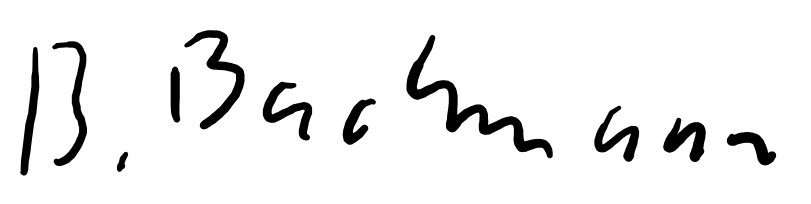
\includegraphics[height=1.5cm,keepaspectratio]{BasilBachmann}\\
	Pascal Baumann & 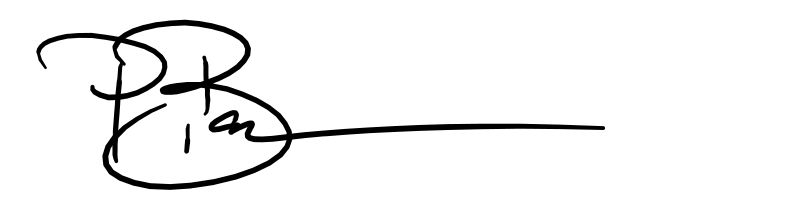
\includegraphics[height=1.5cm,keepaspectratio]{PascalBaumann}\\
	David Craven & 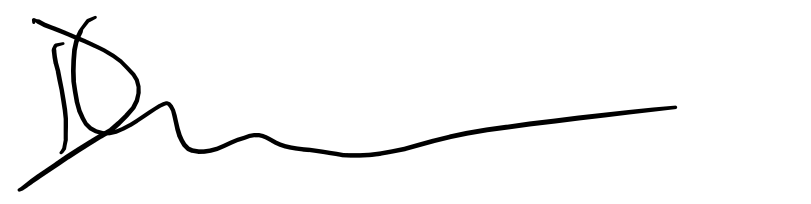
\includegraphics[height=1.5cm,keepaspectratio]{DavidCraven}\\
	Victor Guntern & 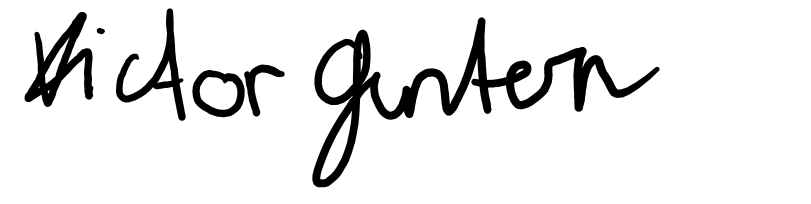
\includegraphics[height=1.5cm,keepaspectratio]{VictorGuntern}\\
	Markus Kempf & 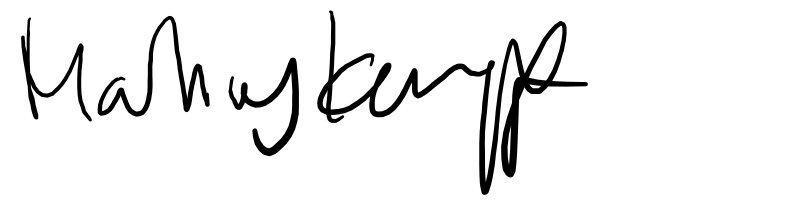
\includegraphics[height=1.5cm,keepaspectratio]{MarkusKempf}\\
	Eve Meier & 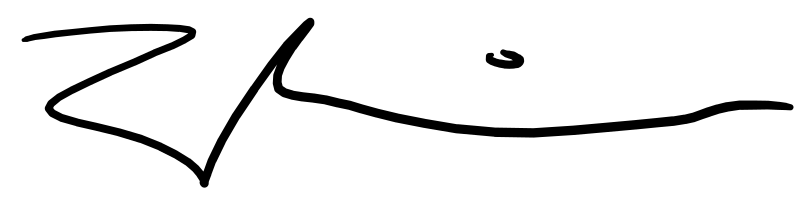
\includegraphics[height=1.5cm,keepaspectratio]{EveMeier}\\
	Jan Odermatt & 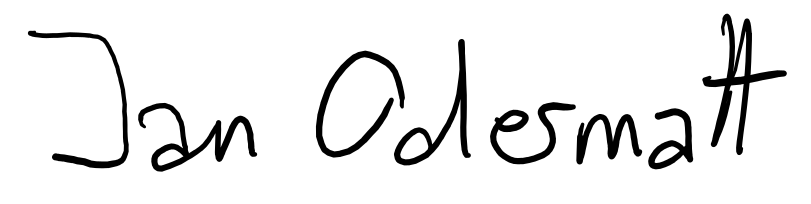
\includegraphics[height=1.5cm,keepaspectratio]{JanOdermatt}\\
	Simon Rohrer &  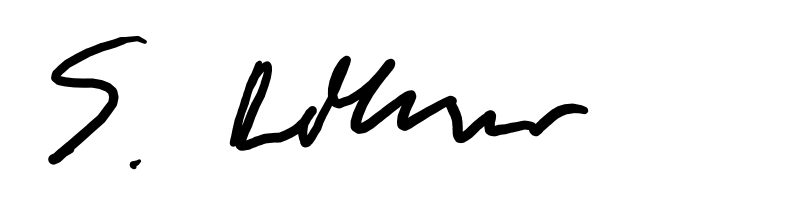
\includegraphics[height=1.5cm,keepaspectratio]{SimonRohrer}\\
\end{tabular}

\newpage

\pagenumbering{roman}
\begin{abstract}
	%TODO Abstract and Summary
	Hier würde man das Abstract oder Management Summary schreiben.
\end{abstract}

\chapter*{Versionierung}
\label{ch*:Vers}
\vspace{2em}

\noindent
\begin{tabular}{|c|p{0.7\textwidth}|}
	\hline
	\textbf{Versionsnummer} & \textbf{Beschreibung}\\
	\hline
	1.0 & Meilenstein 1 \\
	\hline
	2.0 & Meilenstein 2 \\
	\hline
\end{tabular}

\tableofcontents

\newpage

\pagenumbering{arabic}

\chapter{Einleitung}
\label{ch:Intro}
% TODO EVE

Dieses Dokument beschreibt den Entwicklungsprozess einer autonomen Laufkatze. Dabei handelt es sich um ein interdiszpilinäres Projekt, welches über zwei Semester an der Hochschule Luzern absolviert wurde. In diesem Projekt musste mit einem begrenzten Budget gearbeitet und vielseitige Herausforderungen bewältigt werden.

In einer ersten Phase wurden vor allem Arbeitsprozesse ausgearbeitet, Recherchen betrieben und Konzepte entwickelt. Den schon frühen Entscheid mit \LaTeX  die Dokumentation zu gestalten schien zuerst gewagt, die einzelnen Teammitglieder lernten jedoch schnell mit diesem neuen Werkzeug zu arbeiten.

\section{Kurzbeschrieb Anforderungen}
\label{sec:KurzAnforder}
Das Gerät muss sich autonom entlang eines ansteigenden Drahtseil fortbewegen können. Die Last muss an einem fix bestimmten Ort aufgehoben werden, ohne Berührung über die folgenden Hindernisse transportiert und danach möglichst exakt auf einer Zielplatte im Absetzbereich abgesetzt werden (siehe Abb.\ref{fig:Funktionsskizze}). Nach dem Absetzen der Last muss das Gerät den Zielraum erreichen und den Masten berühren. Die Zielplatte muss das Gerät selbstständig erkennen können. Das Gerät darf nur die Last, das Drahtseil und den zweiten Masten berühren. Nach Aufnahme der Last muss die aktuelle Position der Last in x-, und z-Richtung in Echtzeit dargestellt werden. Das Gerät muss innerhalb von zwei Minuten startbereit sein. Die Zeit um den Zielraum zu erreichen liegt bei maximal vier Minuten. In der Abbildung \ref{fig:Ablaufdiagramm} sehen Sie eine anschauliche Darstellung des Ablaufs.
In Abbildung \ref{fig:Blockdiagramm} befindet sich eine Darstellung der technischen Komponenten und ihren Zusammenhängen.

\chapter{Lösungskonzeption}
\label{ch:Loesungskonzept}

\section{Beschreibung der Grundfunktion}
\label{sec:GrundBeschrieb}
% TODO BASIL
Die Grundfunktionen des zu bauenden Gerätes sind hauptsächlich das Fortbewegen an einem Drahtseil und das Greifen und Absetzten einer Last. Um die Last zu Greifen ist ein Hubmechanismus notwendig, der die Last um mindestens 200mm hoch heben kann. Die aktuelle Position der aufzuhebenden Last wird auf dem Gerät mit einem Display angezeigt. Diese Funktionen laufen bis auf das Startsignal autonom ab. Eine Kamera wird verwendet, um die vorgegebene Zielplattform zu erkennen. Damit ist das Gerät in der Lage an der richtigen Position über dem Mittelpunkt der Zielplattform zu stoppen. Um die aktuelle Position anzeigen zu können, wird ein Ultraschallsensor verwendet.

\begin{figure}[h!]
	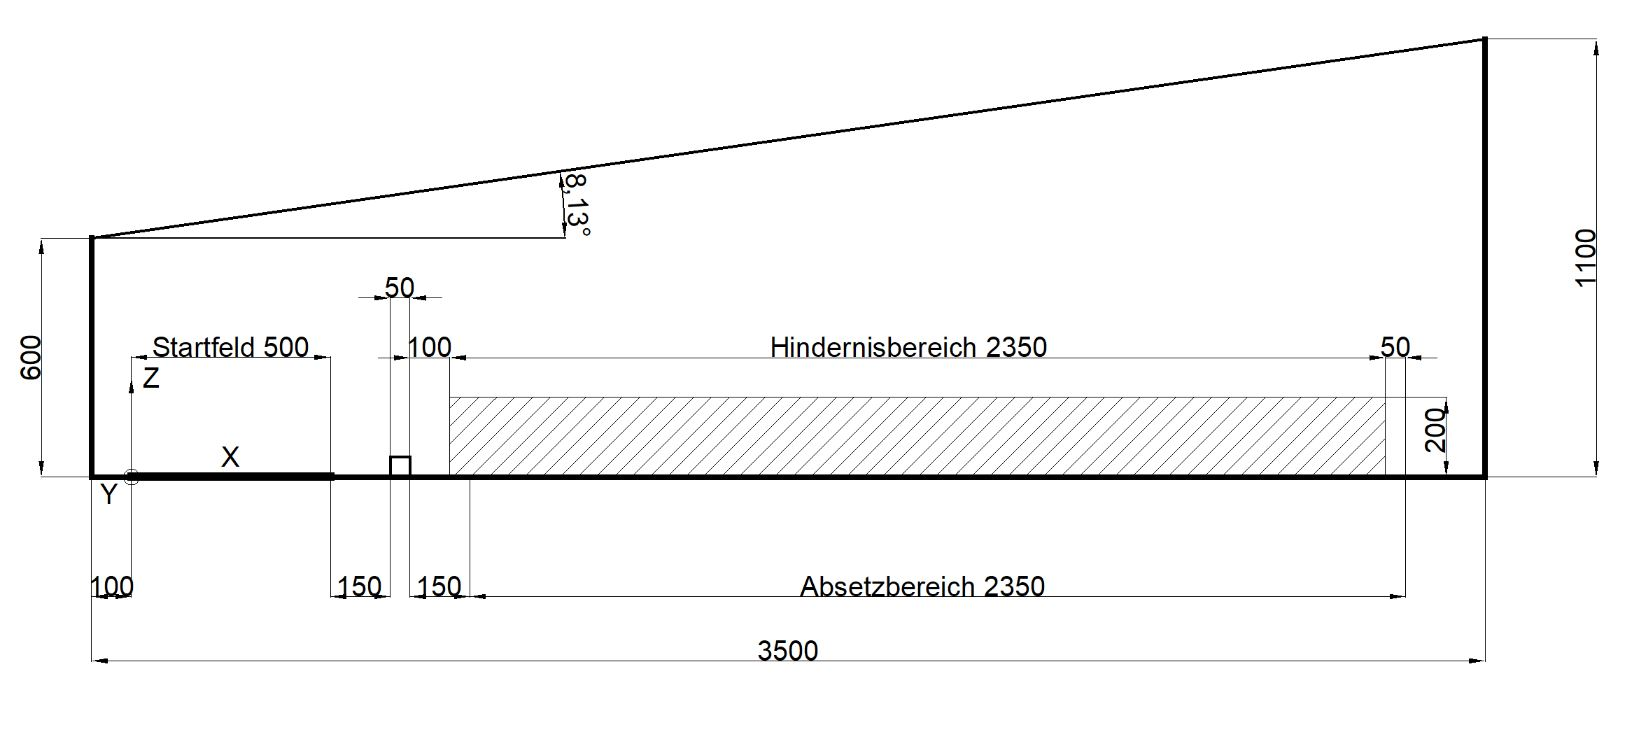
\includegraphics[keepaspectratio,width=\textwidth]{PrenFunktionsskizze}
	\caption{Übersichtsmodell}
	\label{fig:Funktionsskizze}
\end{figure}

\newpage
\section{Ablaufdiagramme}
\label{sec:Ablaufdiagramme}
Der Ablauf der verschiedenen Teilschritte erfolgt gemäss  Abbildung\ref{fig:Ablaufdiagramm}.

\begin{figure}[h!]
	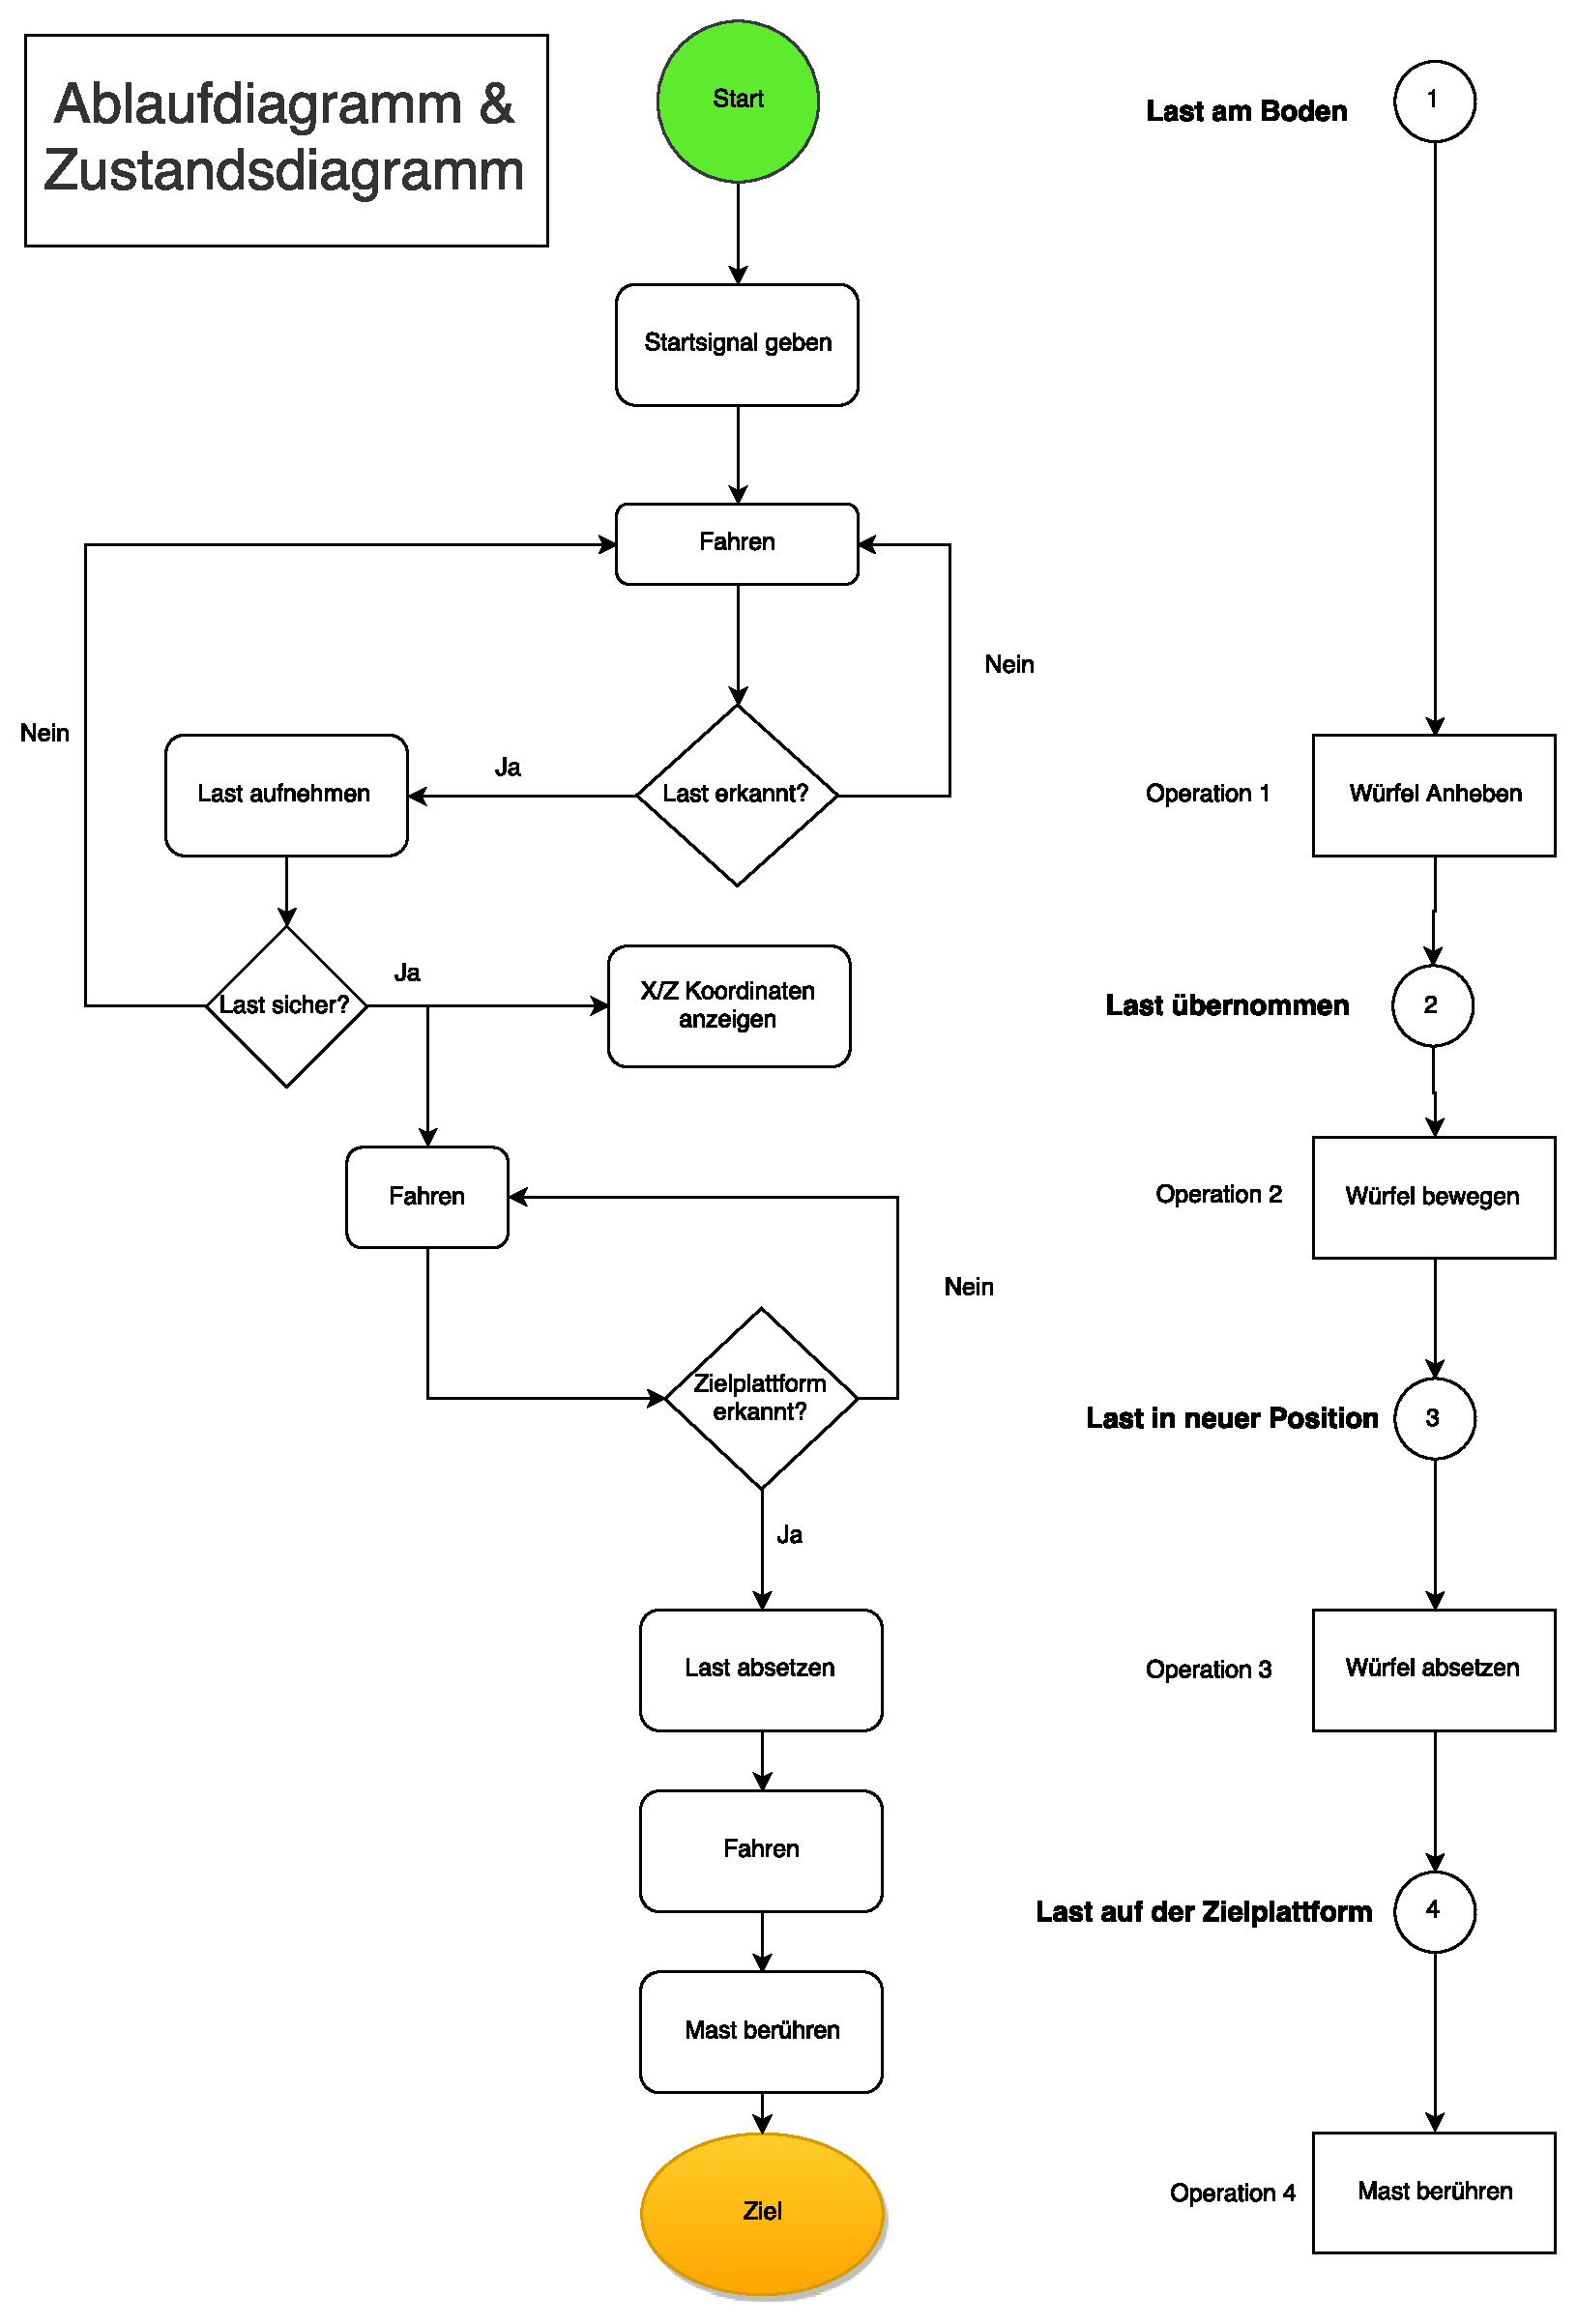
\includegraphics[keepaspectratio,width=\textwidth]{Ablaufdiagramm}
	\caption{Ablauf- und Zustandsdiagramm}
	\label{fig:Ablaufdiagramm}
\end{figure}

Im Blockdiagramm \ref{fig:Blockdiagramm} sind die Schnittstellen graphisch dargestellt.

\begin{figure}[h!]
	\centering
	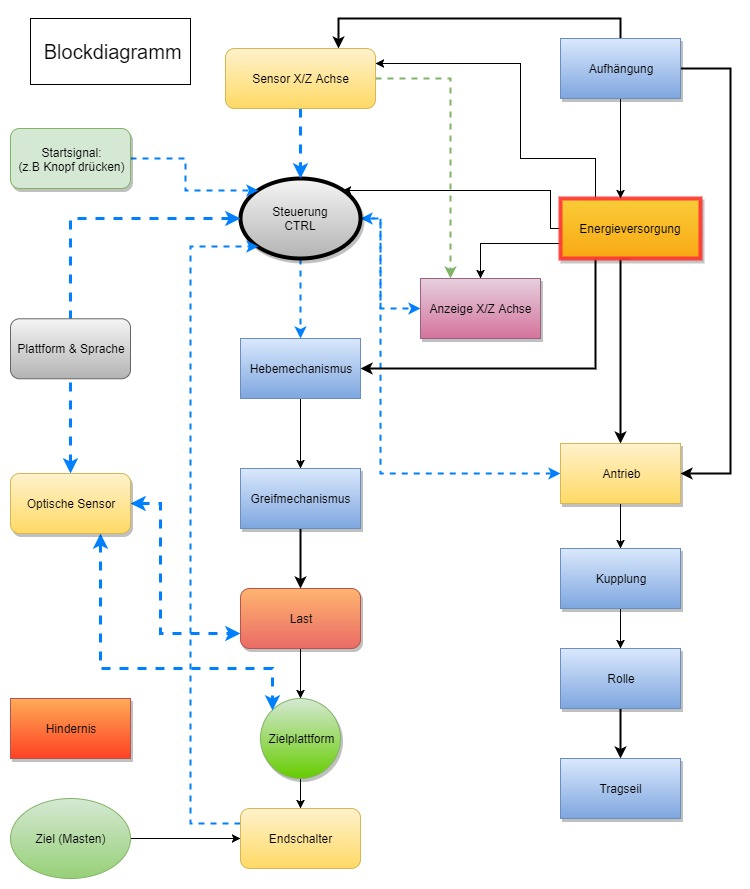
\includegraphics[keepaspectratio,width=\textwidth]{Blockdiagramm}
	\caption{Blockdiagramm}
	\label{fig:Blockdiagramm}
\end{figure}

\section{Beschreibung der Komponenten}
\label{sec:KompBeschrieb}
In diesem Kapitel werden die Komponenten unseres Konzepts genauer beleuchtet. Auf Abbildung \ref{fig:LoesungsKonzept} sind diese markiert.

\begin{figure}[h!]
	\centering
	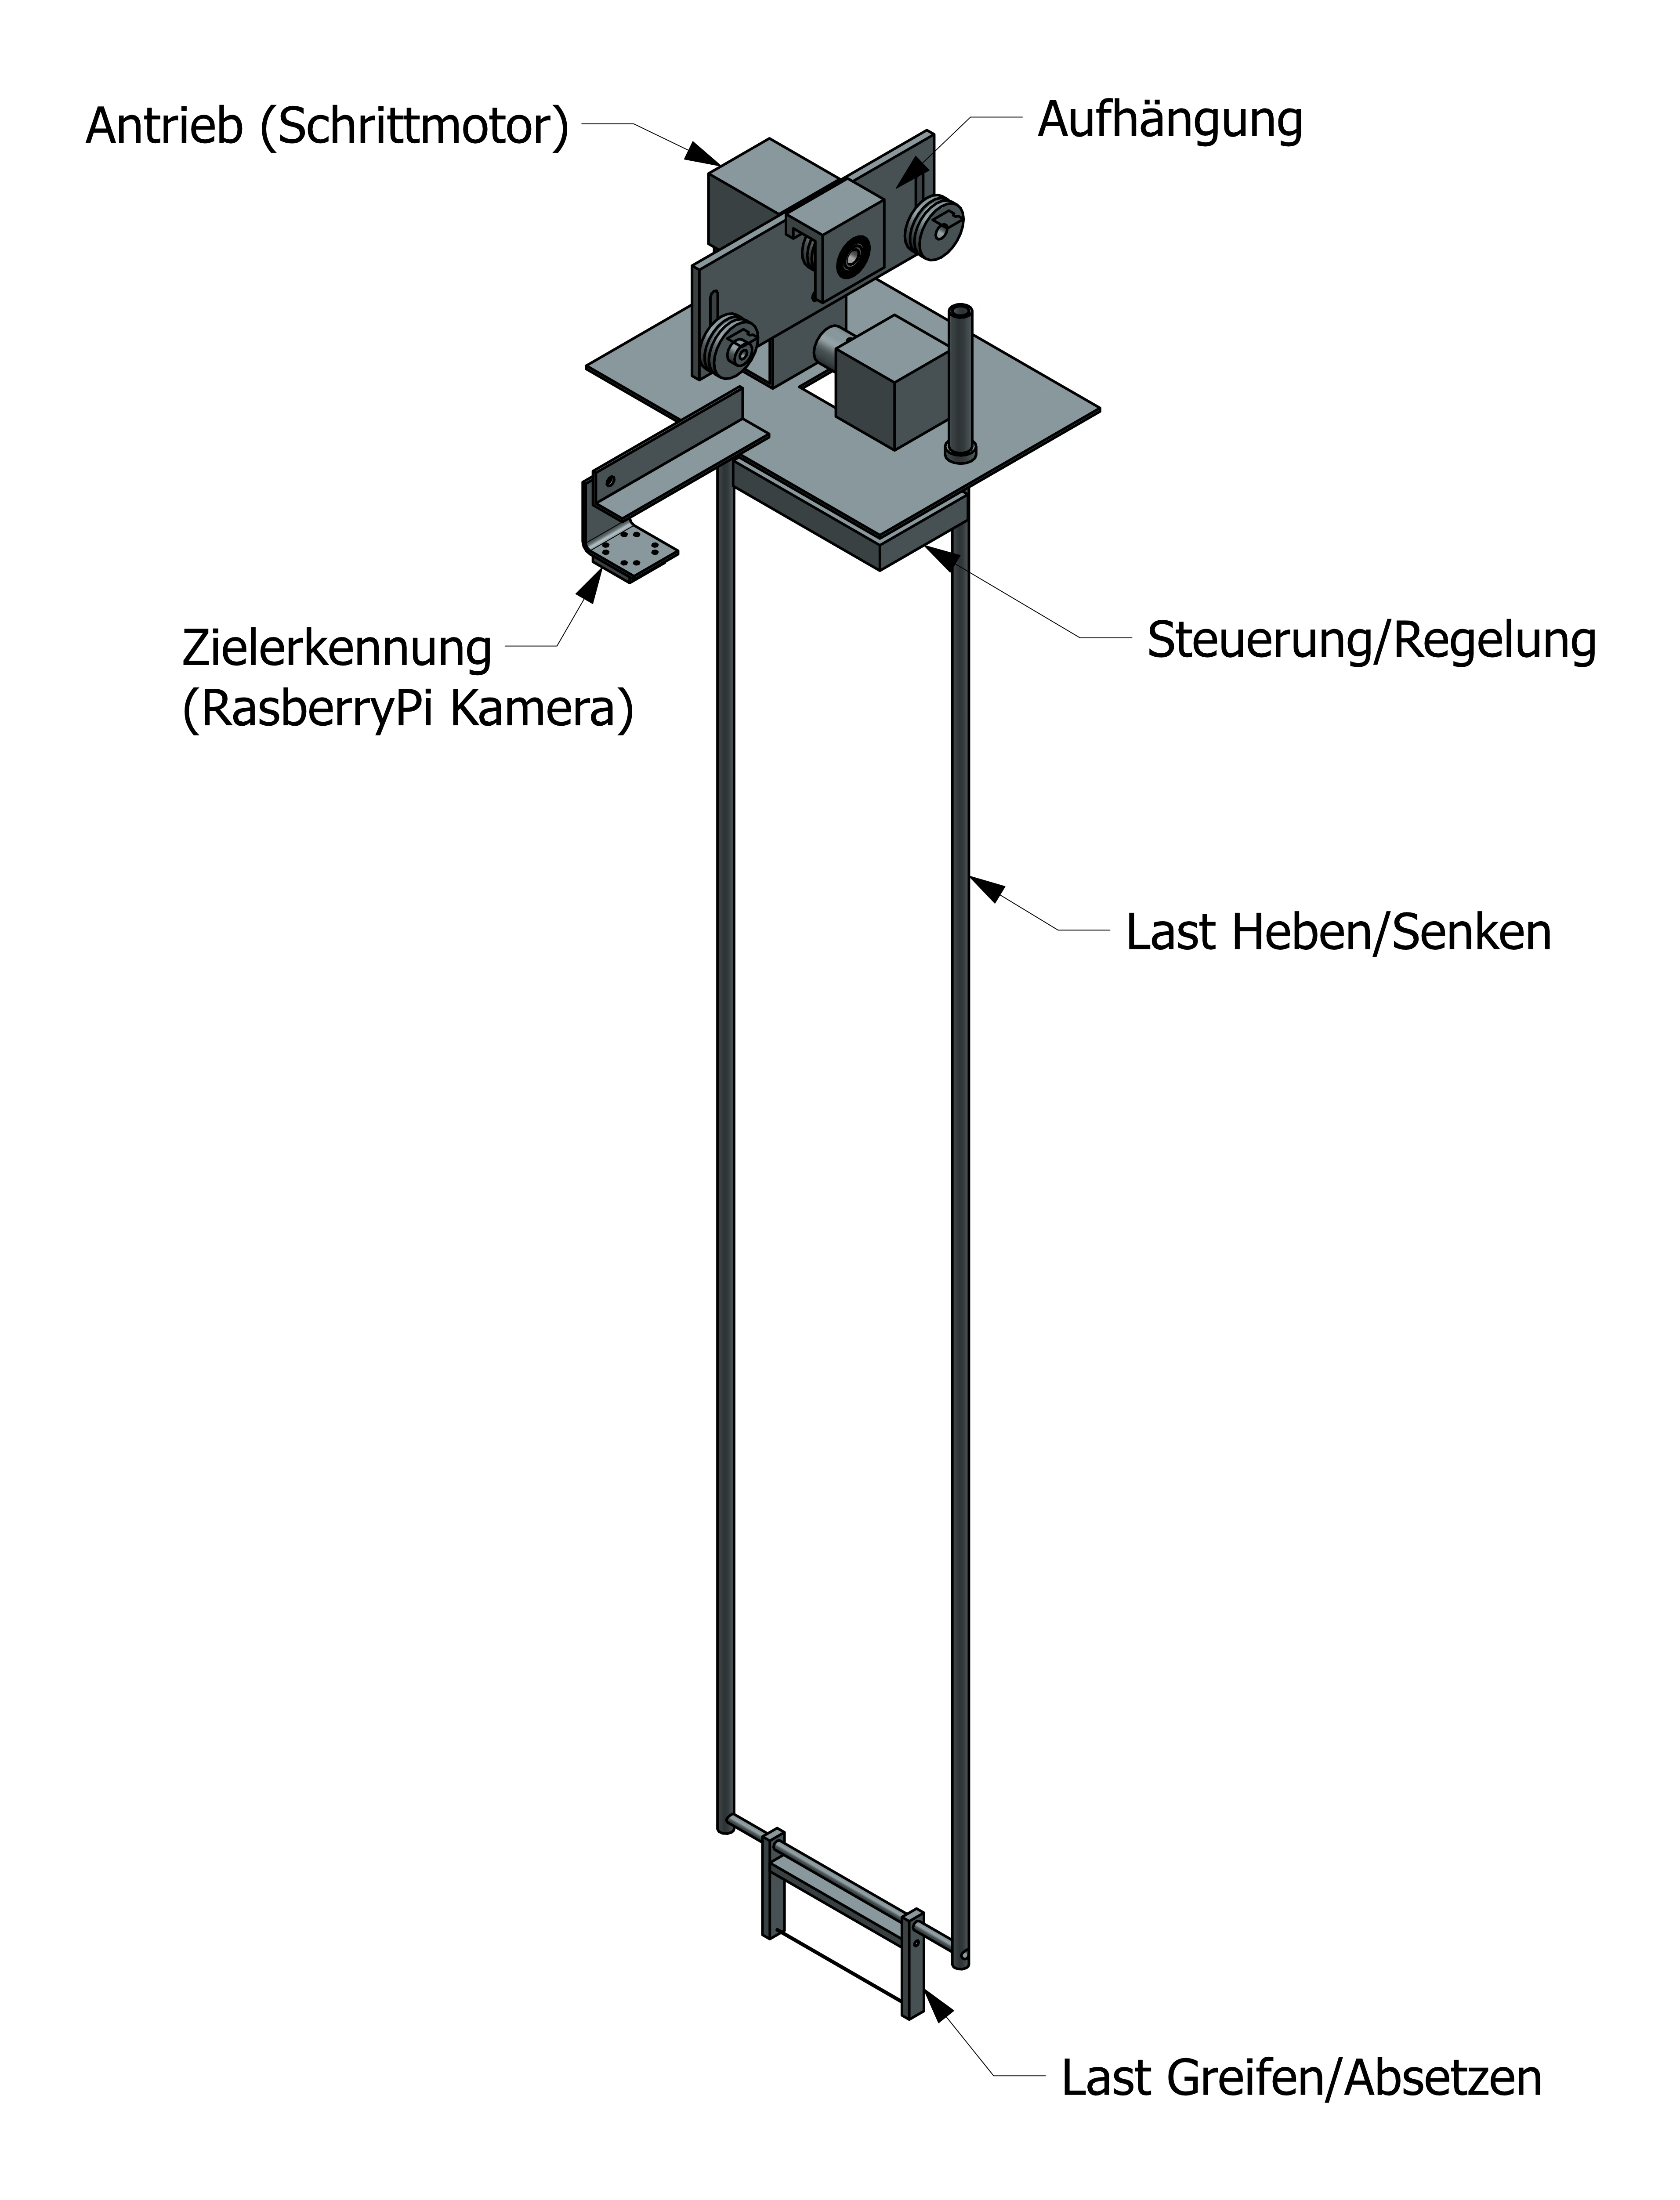
\includegraphics[height=0.5\textheight,keepaspectratio]{marku_103000_bg-00_ze1}
	\caption{Skizze unseres Lösungskonzeptes}
	\label{fig:LoesungsKonzept}
\end{figure}

\newpage

\subsection{Aufhängung}
Durch die unten gelenkige und gedämpft gelagerte Aufhängung kann die Winkeländerung, welche durch den Seildurchhang verursacht wird, kompensiert werden. Dabei hängt die Last durch den Schwerpunkt immer senkrecht nach unten. Durch das Gelenk (ähnlich wie bei einer Gondelbahn) wird der ganze Aufbau aber empfindlich gegen pendeln, weil das Gelenk kein Drehmoment aufnehmen kann. Dieses wird beispielsweise durch die Beschleunigung bei Anfahren oder Abbremsen erzeugt. Das Gelenk wird durch zwei Löcher und eine Schraube mit einer Sicherungsmutter realisiert. Zudem kann sich, je nach Aufbau, der Schwerpunkt der Laufkatze beim Anheben und Absetzen der Last ändern, was wiederum ein Drehmoment erzeugt. Mit Dämpfern kann das Drehmoment aufgenommen und ein Pendeln minimiert werden. Diese Dämpfer werden dann, im Prinzip einer Pendelstütze in der Mechanik, am einen Ende am Antrieb und am anderen Ende an der Aufhängung montiert. Zudem soll der Dämpfer möglichst horizontal angestellt sein, damit er die Pendelbewegung aufnehmen kann. In der Aufhängung werden der Hubmotor, die elektrischen Komponenten, der Energieversorgung und die Führungen der Hubeinrichtung angebracht. Diese besteht aus zwei Linearführungen, wobei zwei Stäbe in einem Rohr hoch und hinuntergefahren werden. Weiter werden je nach Notwendigkeit Ausgleichsgewichte auf der Aufhängung positioniert, damit die Laufkatze zentral unter dem Seil hängt. Die Aufhängung wird komplett aus Aluminium gefertigt.

\subsection{Antrieb}
Der Antrieb auf dem Seil wird mit drei Räder aus Aluminium ausgeführt. Das mittlere Rad ist das angetriebene Rad. Es wird direkt von einem Schrittmotor angetrieben. Dies setzt voraus, dass die Achse des Motors um den Radius des Antriebsrades über dem Seil sein muss. Dies hält die Ausfallwahrscheinlichkeit tief, da keine Riemen-, oder Zahnradübersetzung notwendig. Zudem kann auch der Schlupf klein gehalten werden. Weil der Motor aber über dem Seil liegt, ist auch der Schwerpunkt des gesamten Gerätes höher. Dies macht den Lastausgleich schwieriger und begünstigt Schwingungen.\\
Vor-, und hinter dem Antriebsrad sind im Abstand von 5cm zwei Führungsräder angebracht. Diese sind in der Höhe verstellbar und müssen manuell im voraus eingestellt werden. Die Aufgabe dieser Räder ist die Schwingung in x-Richtung zu minimieren und den Druck des Seiles auf das Antriebsrad zu erhöhen. Letzteres hat zur Folge, dass der Reibwert sich erhöht und somit der Schlupf und die Gefahr auf Rutschen auf dem Seil zu vermindern. Um den Reibwert zusätzlich zu erhöhen, ist die Laufrille des Antriebsrades aus Aluminium mit einer Gummibeschichtung versehen.


\subsection{Regelung und Steuerung}

Als Kern der Elektronischen Steuerung wird das LoFive Board verwendet, welches mit dem SiFive Freedom E310 Microprozessor bestückt ist. Dieser wurde nach dem offenen Standart der RISC-V Foundation konstruiert und ist daher für jeden einsehbar. Als Programmiersprache wird voraussichtlich Rust verwendet.

Vom Board werden zwei Schrittmotoren-Treiber sowie ein LCD-Display angesteuert. Zur Rückmeldung wird ein Ultraschallsensor und das RasPi verwendet.

Weil die Steuerung vom RasPi die Richtung und Distanz zur Zielplattform übermittelt kann das System als Regelungssystem betrachtet werden. Solange das Ziel nicht erkannt wird, soll das Gerät mit maximaler Geschwindigkeit fahren. Mit der erkennung des Ziels wird das Gerät längers wie langsamer und stoppt über dem Zielfeld. Mit diesem System wird ein effektives Anfahren des Ziels erreicht. Zum Starten und Stoppen des Geräts wird ein Schalter und ein Taster verwendet.

\subsection{Positionsanzeige}

Auf dem Display wird die X- sowie die Z-Koordinate dargestellt. Die X-Koordinate wird mithilfe des Schrittmotors und zusätzlich mit einem Ultraschall-Distanzsensor bestimmt werden. Die Z-Koordinate wird mit einer Durchhangstabelle und dem Schrittmotor erfasst. Das Entwicklungsteam ist sich bewusst, dass Schrittmotoren einerseits Schritte überspringen könnten und die mechanische Umsetzung gleiten kann. Jedoch wird davon ausgegangen, dass der Motor beim Lastanheben keine Schritte überspringt.

\newpage
\subsection{Zielerkennung}
\subsubsection{Systemübersicht}

\begin{figure}[h!]
	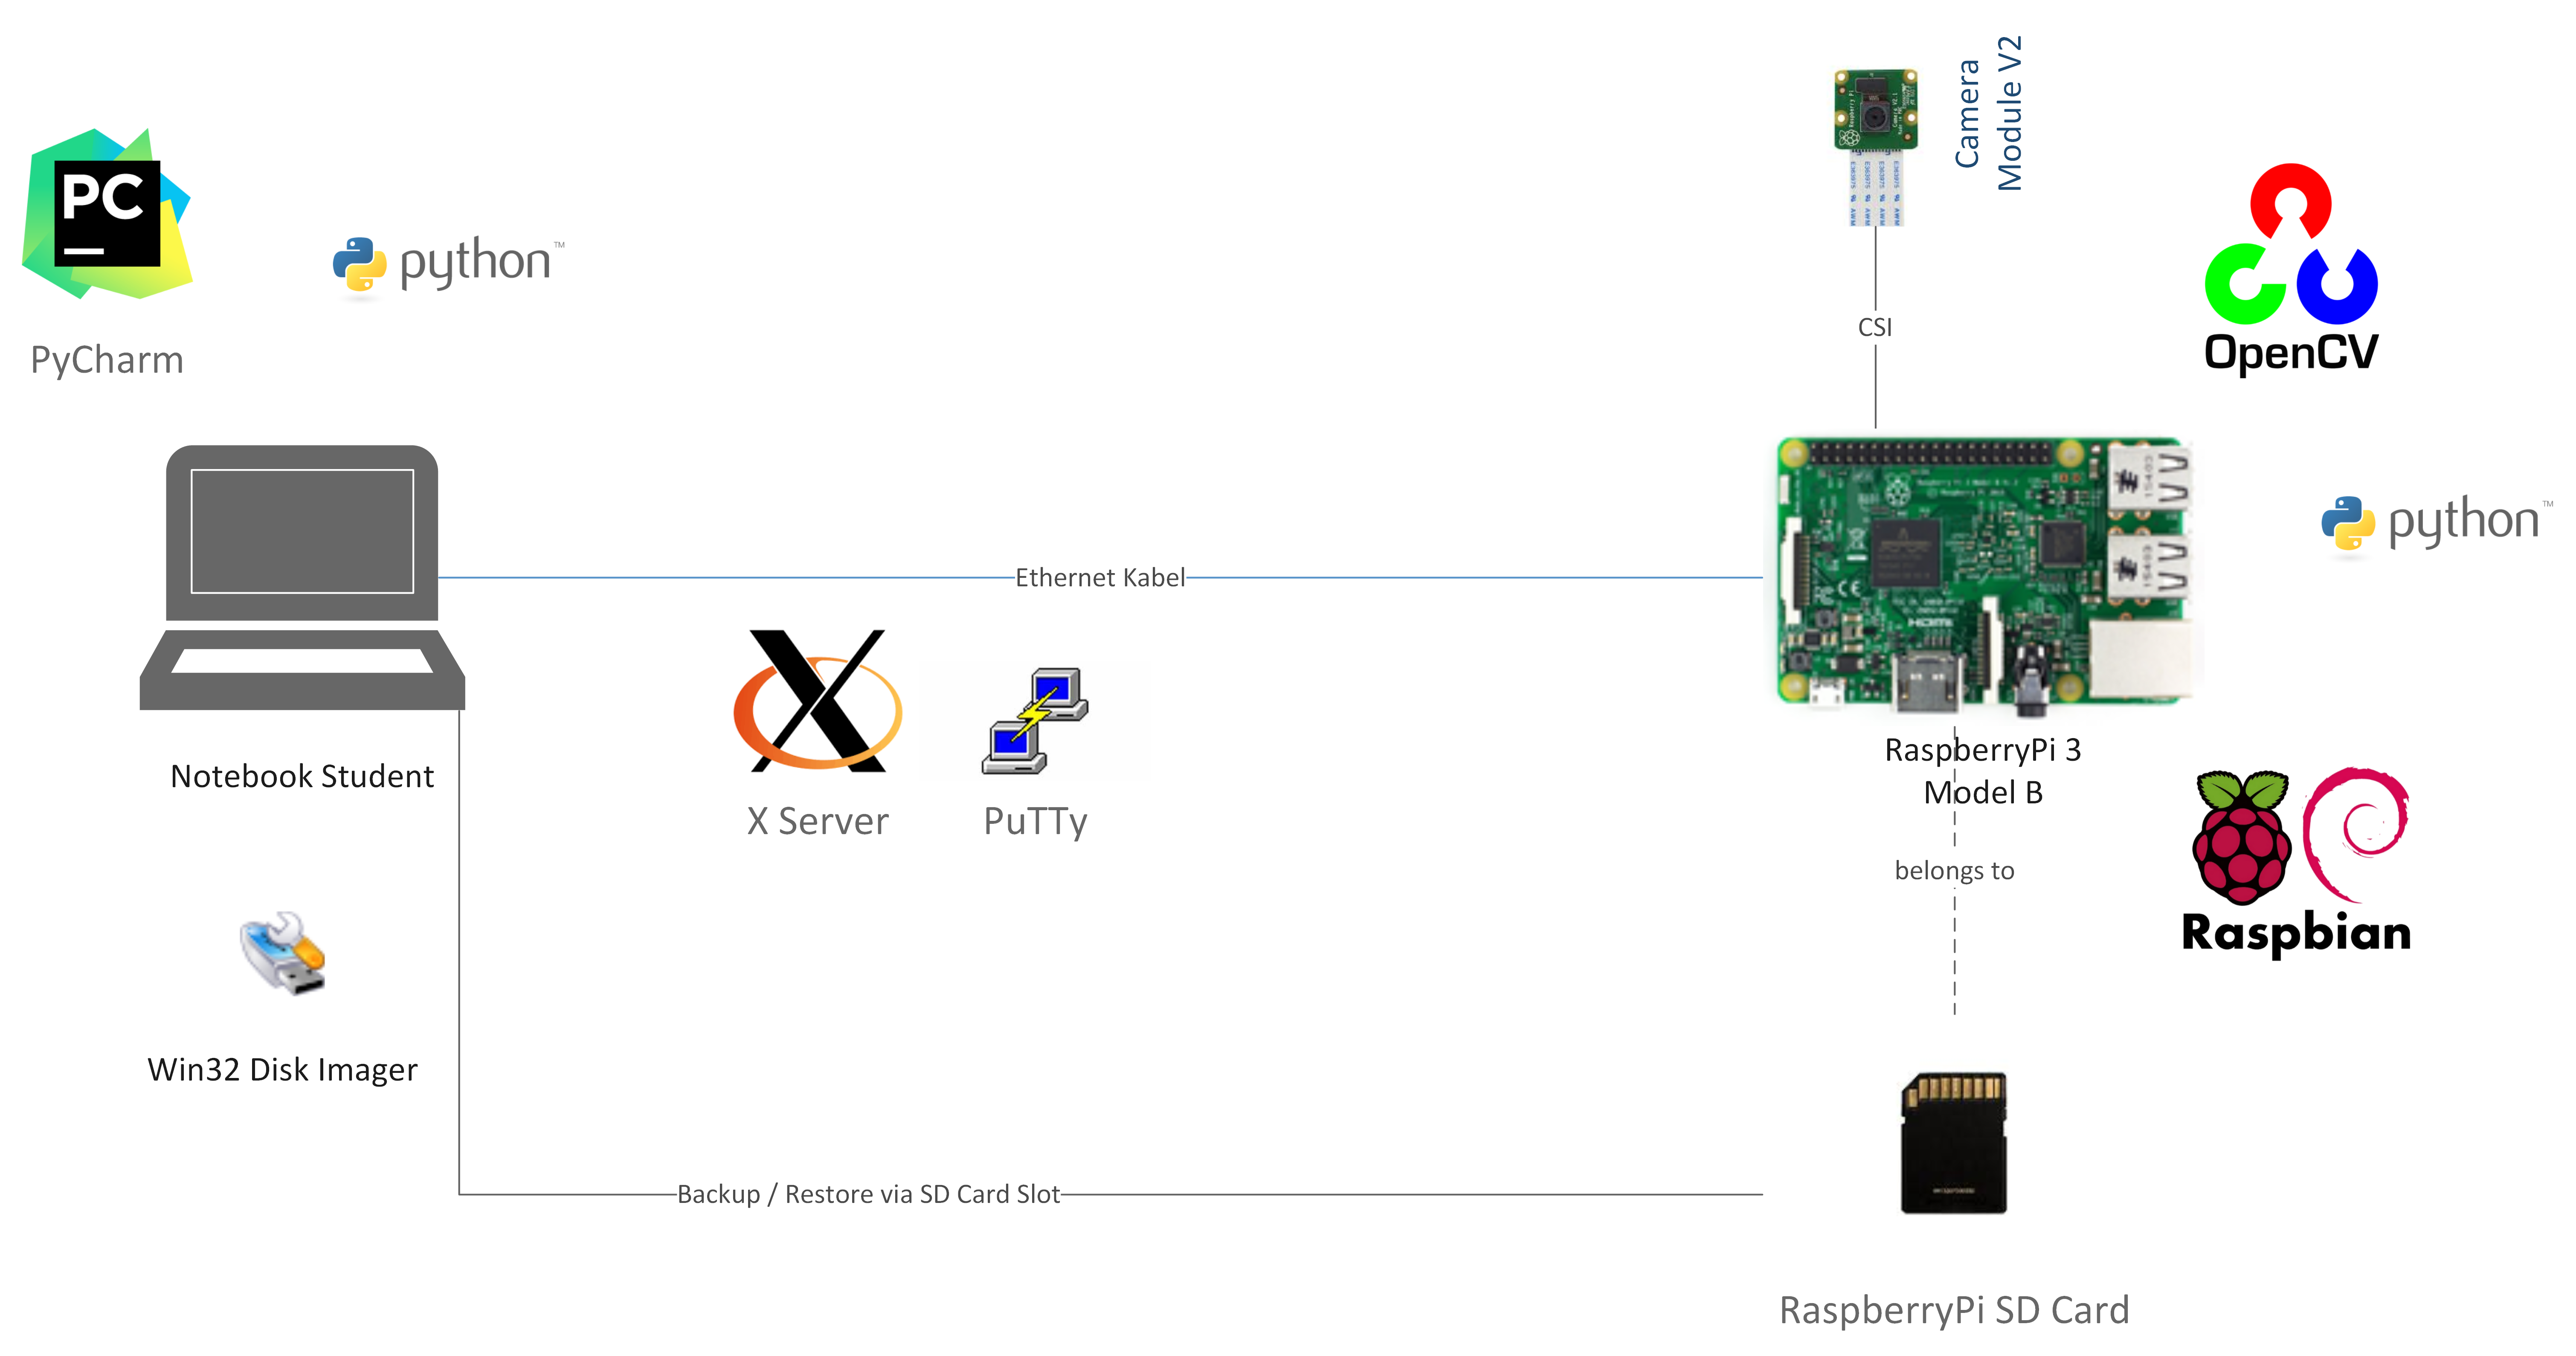
\includegraphics[keepaspectratio,width=\textwidth]{TargetRecOS}
	\caption{Systemübersicht}
	\label{fig:Systemuebersicht}
\end{figure}

Das Raspberry Pi ist ein Einplatinencomputer in der Grösse einer Kreditkarte. Das Ein-Chip-System von Broadcom läuft mit einem ARM-Mikroprozessor. Durch seine Bekanntheit, der vielen Module die es dazu fertig gibt, sowie seinem Preis ist das Raspberry Pi Pionier auf dem Bereich der Einplatinencomputer.

\begin{itemize}[noitemsep]
	\item Quad Core 1.2GHz Broadcom BCM2837 64bit CPU
	\item 1GB RAM
	\item BCM43438 WLAN und Bluetooth Low Energy (BLE) auf dem Board
	\item 40-pin erweitertes GPIO
	\item 4 USB2 Ports
	\item 4 Pol Stereo Ausgang und Composit Video Port
	\item Full-Size HDMI
	\item CSI Kamera Port um eine Raspberry Pi Camera anzuschliessen
	\item DSI Bildschirmausgang um einen Raspberry Pi Touchscreen anzuschliessen
	\item MicroSD Anschluss um das OS und Daten zu speichern
	\item Die geschaltete Micro USB Stromzufuhr wurde auf bis zu 2.5A erhöht
\end{itemize}\parencite{RaspberryPiFoundation2017}

\vspace{1em}
Auf dem RaspberryPi wird als Grundinstallation das Betriebssystem Raspian installiert. Darauffolgend werden Module für Python (Version 2) und OpenCV (Version 3) für die Bilderkennung hinzugefügt.
Um auf das RaspberryPi zugreifen zu können wird einerseits PuTTy benutzt, um eine SSH Verbindung aufzubauen. Andererseits benötigen wir X Server für das Streaming des Kamerabildes.
Um den aktuellen Stand (das Abbild, Image) des RaspberryPi zu speichern und gegebenenfalls wiederherstellen zu können, wird die SD Karte in ein Studentennotebook gelegt und mithilfe Win32 Disk Imager kopiert.

Auf dem jeweiligen Notebook wird PyCharm als IDE benötigt. In PyCharm wird mit Python programmiert.

Das System muss den Ablauf in Abbildung \ref{fig:AblaufZielerkennung} umsetzen können.

\begin{figure}[h!]
	\centering
	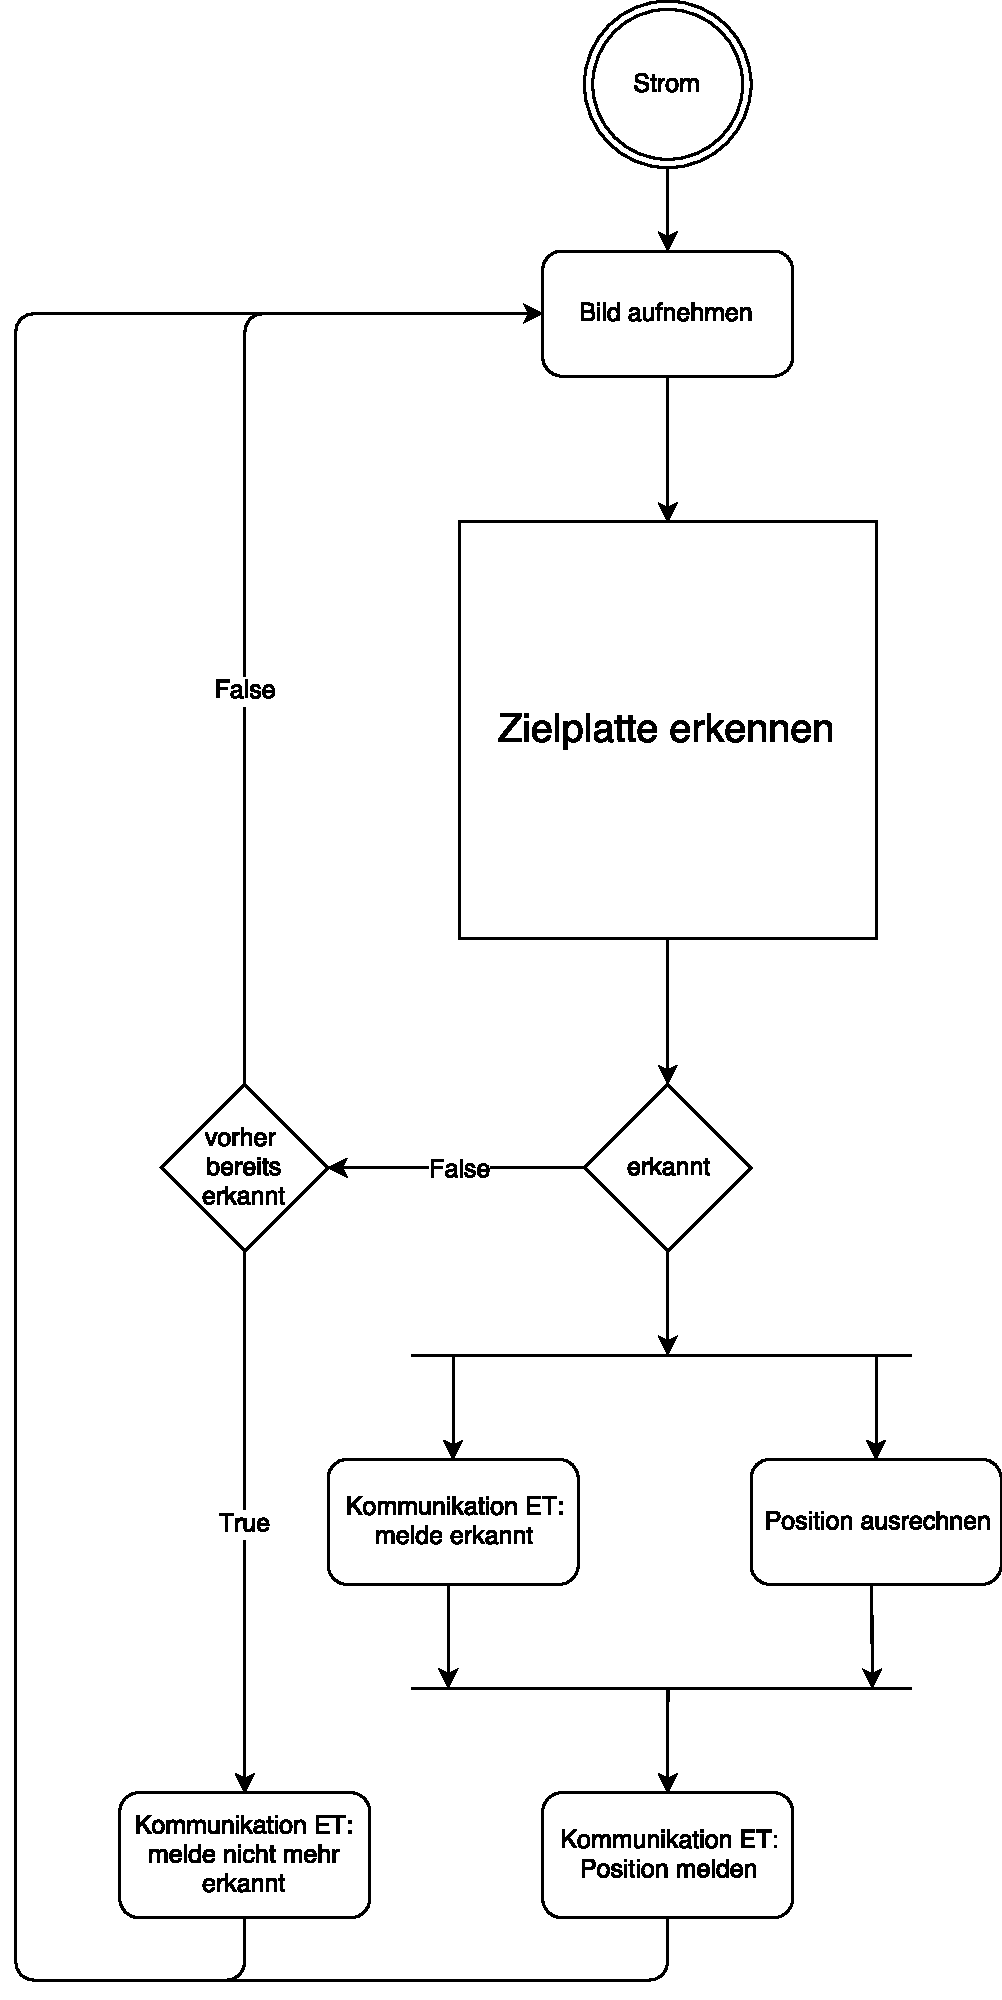
\includegraphics[keepaspectratio,height=0.8\textheight]{Ablaufdiagramm_ModusOperandi}
	\caption{Ablaufdiagramm Zielerkennung}
	\label{fig:AblaufZielerkennung}
\end{figure}

Die Schritt \textquotedblleft Zielplatte erkennen\textquotedblright\ sowie \textquotedblleft Position berechnen\textquotedblright\ werden im Kapitel \ref{ssec:bilderkennung} ausführlich beschrieben.

Jene Schritte mit der Bezeichnung \textquotedblleft Kommunikation ET\textquotedblright\ werden im Kapitel \ref{ssec:kommunikation} detailliert beschrieben.

\subsubsection{Bilderkennung}
\label{ssec:bilderkennung}

\begin{figure}[h!]
	\centering
	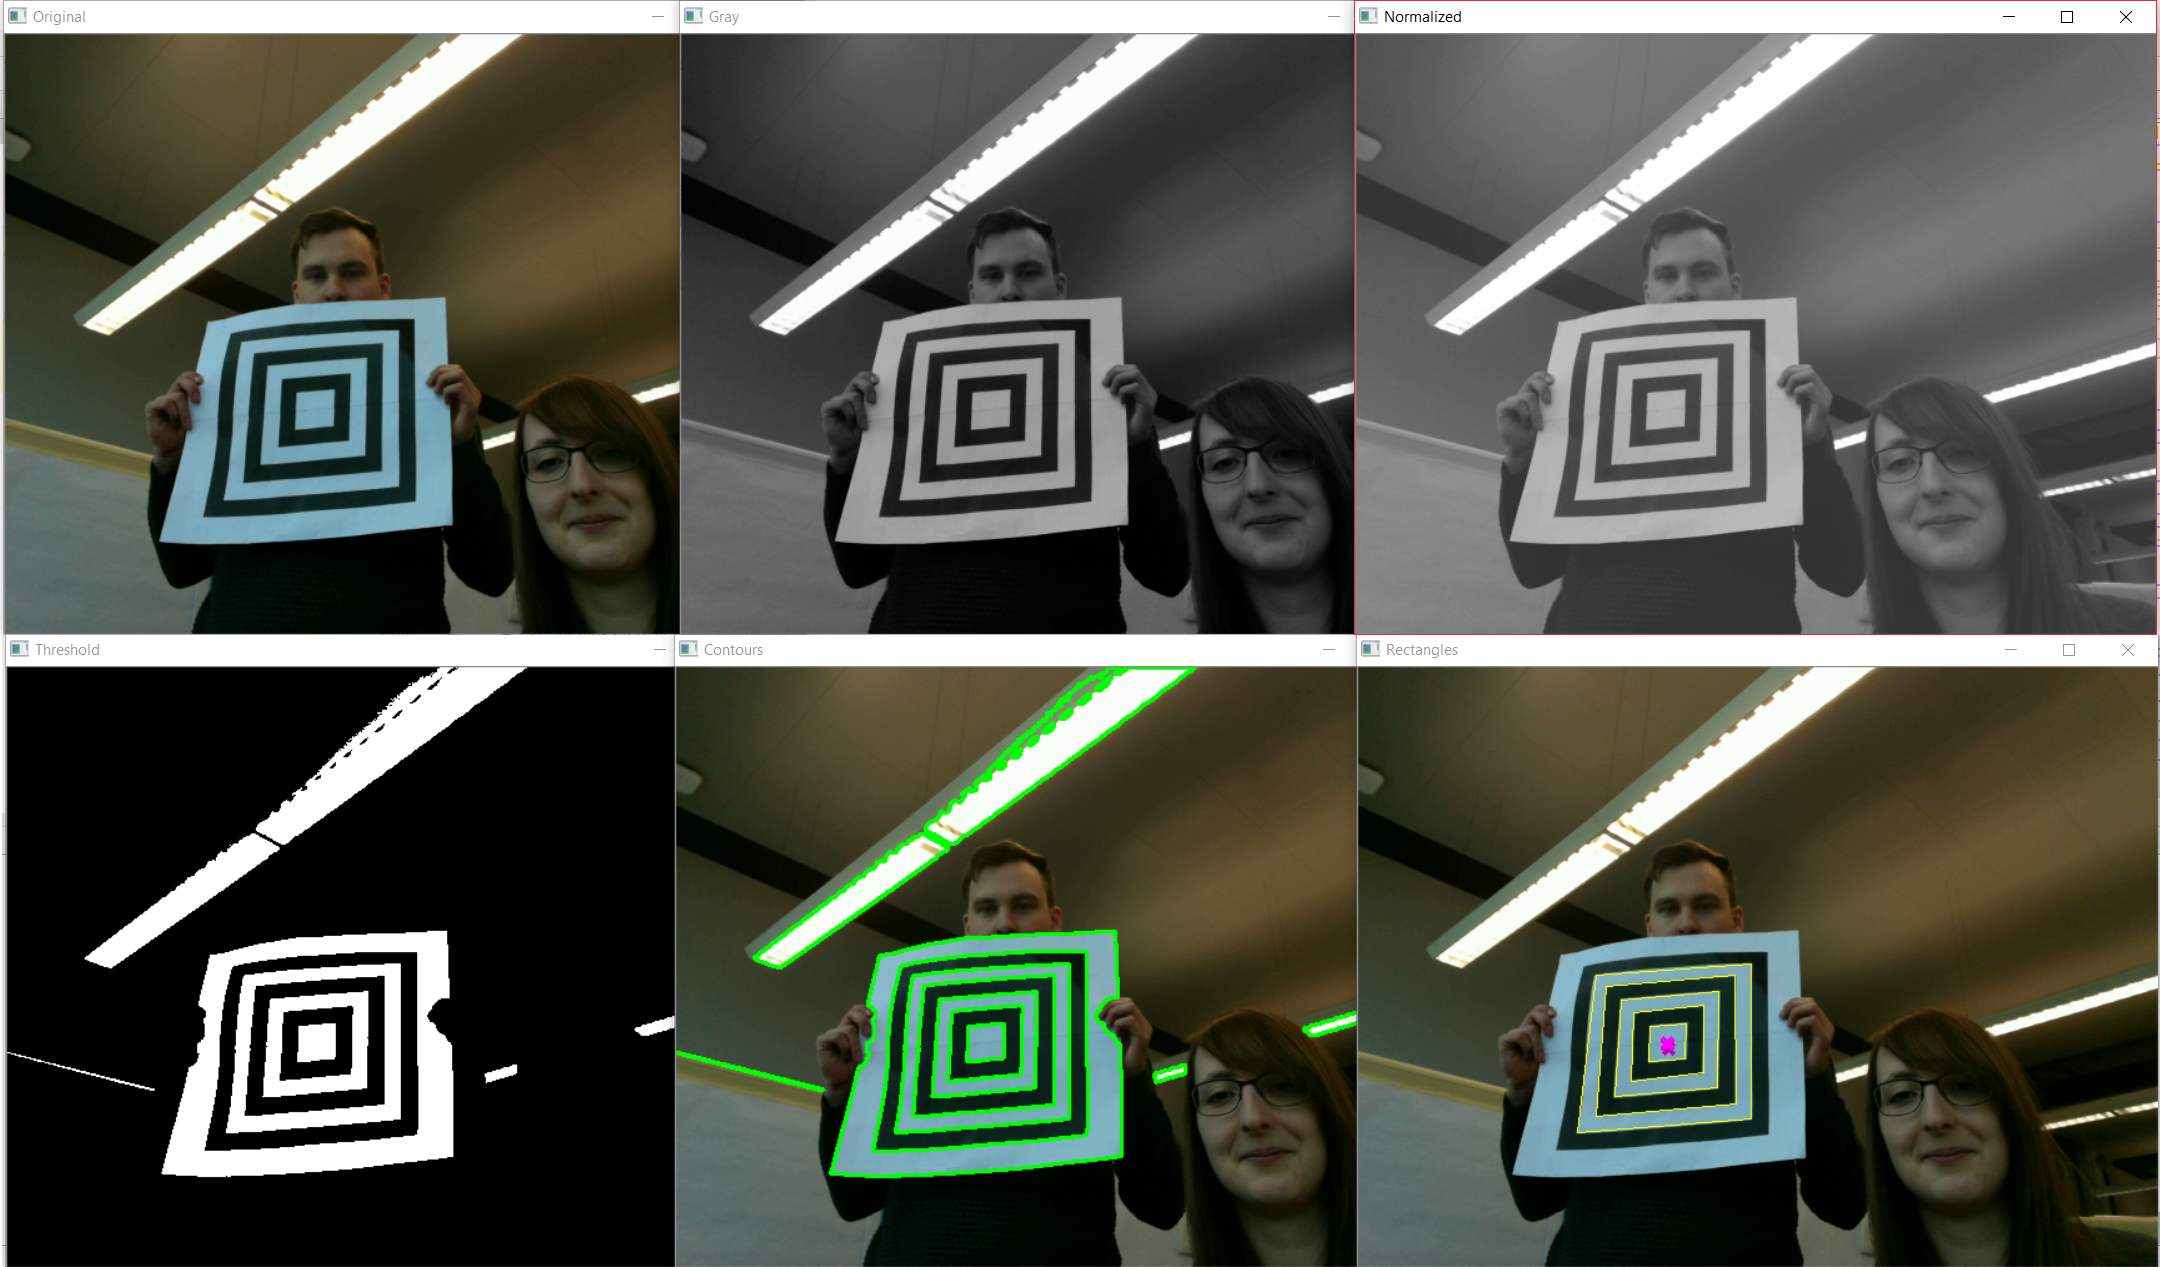
\includegraphics[keepaspectratio,width=\textwidth]{BilderkennungAblauf}
	\caption{Aufnahmen der einzelnen Schritte der Zielerkennung}
	\label{fig:AufnahmeZielerkennung}
\end{figure}

Die Erkennung (in Abbildung \ref{fig:AufnahmeZielerkennung} dargestellt) läuft wie folgt ab:

\begin{itemize}[noitemsep]
	\item[-] Videoframe aufnehmen
	\item[-] Frame in Graustufen umwandeln
	\item[-] Helligkeit durch CLAHE\footnotemark normalisieren
	\item[-] Binären Schwellenwertfilter anwenden
	\item[-] Konturen ausfindig machen
	\item[-] Polygone ausfindig machen
	\item[-] Nur Rechtecke weiter beachten
	\item[-] bestimmte Anzahl Rechtecke mit dem gleichen Mittelpunkt ausfindig machen
	\item[-] Zielplatte erkannt
\end{itemize}

\footnotetext{contrast limited adaptive histogram equalization}

Dieser Ablauf wird in Abbildung \ref{fig:ZielerkennungAblauf} noch genauer dargestellt.

\begin{figure}[h!]
	\centering
	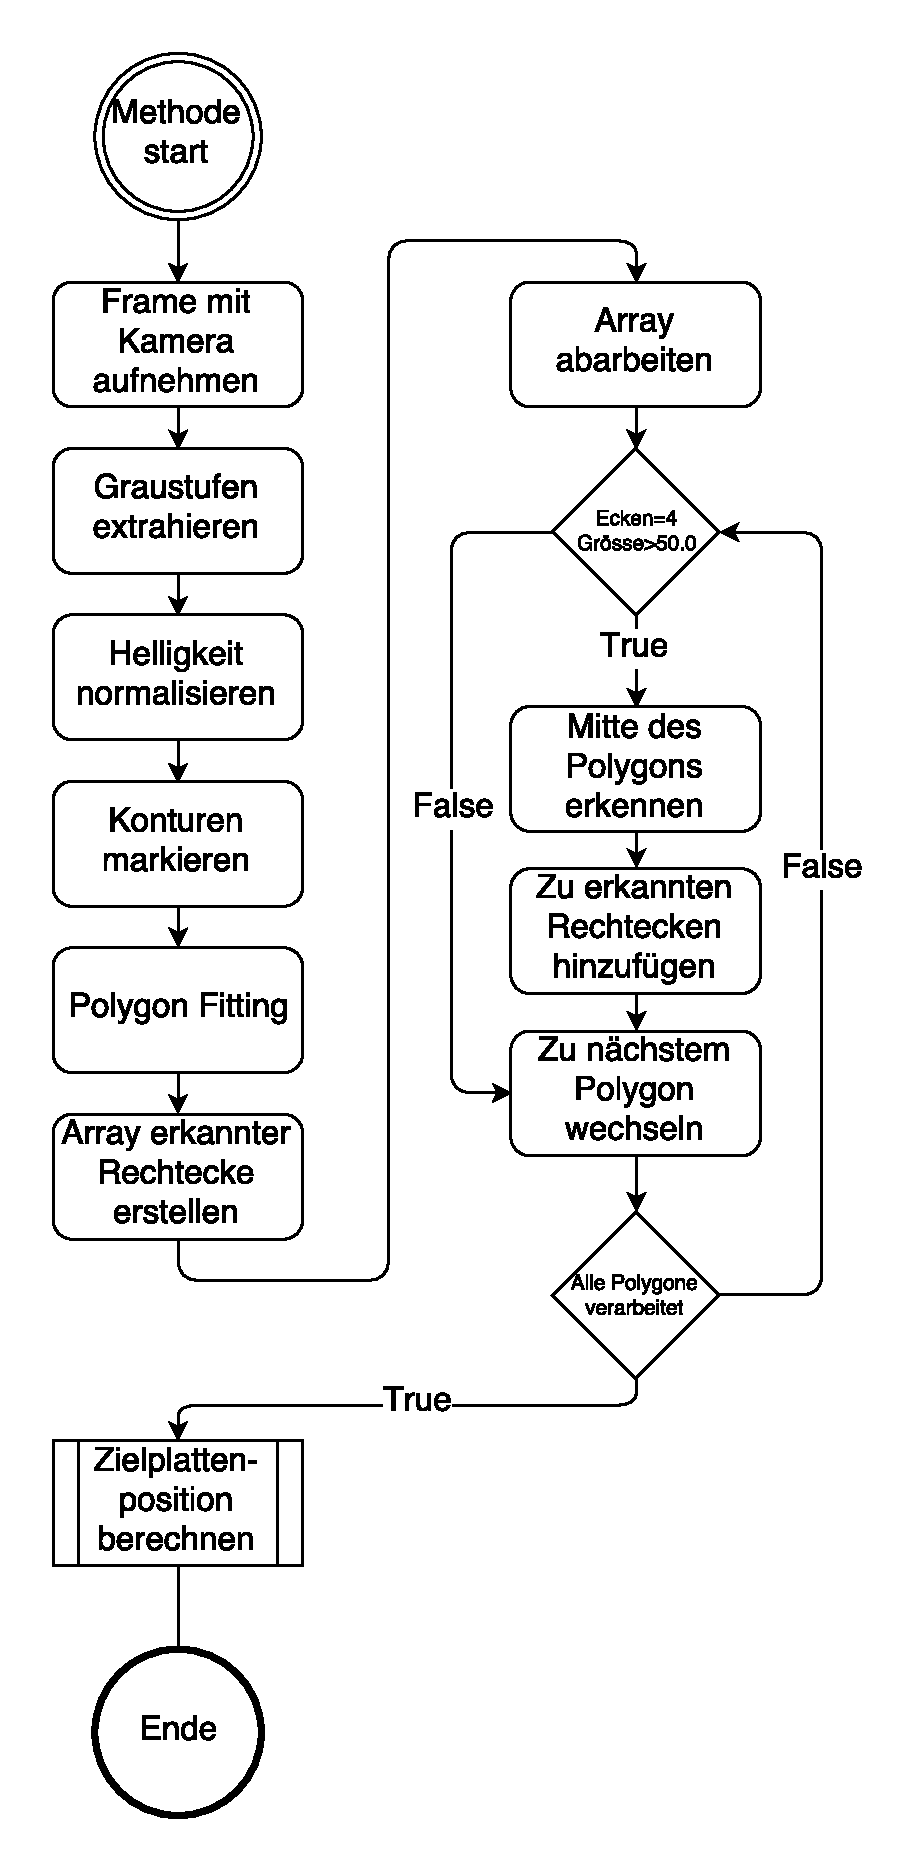
\includegraphics[keepaspectratio,height=0.6\textheight]{ZielplatteErkennen}
	\caption{Ablaufdiagramm Zielerkennung}
	\label{fig:ZielerkennungAblauf}
\end{figure}

\newpage

\subsubsection{Kommunikation zwischen Boards}
\label{ssec:kommunikation}
Zwischen dem RaspberryPi und dem Elektronikerboard soll der Informationsaustausch über eine serielle Schnittstelle erfolgen.

Für die Verwendung einer Kommunikation mit einer asynchronen, seriellen UART-Schnittstelle können jeweilige PINs verwendet werden.

Wie in Abb. \ref{fig:RaspberryPins} dargestellt sind dies Pin 8 (Tx) und Pin 10 (Rx).
\begin{figure}[h!]
	\centering
	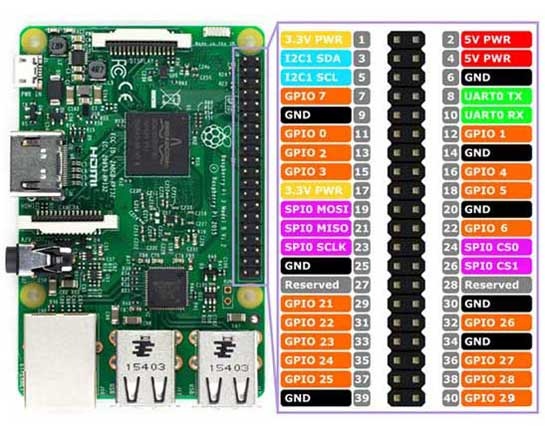
\includegraphics[keepaspectratio, width=0.7\textwidth]{raspberry_pi3_model_b_pin_diagram.jpg}
	\caption{RaspberryPi Pin Diagram}
	\label{fig:RaspberryPins}
\end{figure}

Die Pins können für Testzwecke direkt via Kabel miteinander verbunden werden. Im Endausbau soll diese Verbindung jedoch über einen eigenes angefertigten Print laufen. So wird auch sichergestellt, dass beide Boards einen gemeinsamen GROUND haben.

UART muss auf dem RaspberryPi manuell aktiviert werden.  Zusätzlich muss das integrierte Bluetooth-Modul deaktiviert werden, sodass die genannten Ports nicht "miniUART"\ verwenden.

Für die serielle Übertragung müssen Baudrate, Port, Databits, Parity Check, Stopbits und flow control sowie ein genaues Nachrichtenformat definiert werden. Die Programmierung dieser findet auf dem RaspberryPi mit Hilfe des Python Moduls "pySerial" realisiert.

\newpage

\subsection{Last greifen und absetzen}
% TODO Verweis auf Versuch

Das Greifen der Last erfolgt über einen gelenkig gelagerten Haken. Die gelenkige Lagerung ermöglicht einen grösseren Toleranzbereich in Richtung Z-Achse zum anheben der Last. Versuche haben gezeigt, dass bei Berührung der Last der Greifer nach hinten gekippt wird und durch das Vorwärts bewegen des Fahrzeuges sich in den Hacken der Last einfädelt. Durch einen gekrümmten Draht an der Unterseite des Greifers wird sicher gestellt, dass die Last nach dem Anheben mittig zentriert und durch die Fahrt nicht verschoben wird.

Nachdem das Fahrzeug die Zielplattform erreicht hat, wird die Last vorsichtig abgesetzt. Das Ausfädeln des Drahtes aus dem Haken erfolgt durch eine Rückwärtsbewegung des Fahrzeuges.\\
Der Greifer wird aus Aluminium gefertigt. Dieser besteht aus gebogenem Flachmaterial, durch welchen im oberen Bereich eine Drehachse und im unteren Bereich ein gebogener Draht durch ein Loch geführt wird. Die Drehachse dient zudem noch als Befestigung des Greifers an die Hubvorrichtung.

\subsection{Last anheben und senken}
Die Last wird mithilfe einer Seilwinde angehoben, welche mit einem Schrittmotor angetrieben wird. Dieser ist auf der Befestigungsplatte positioniert. Auf der Motorachse ist eine Seiltrommel aus Aluminium befestigt, welche einen Nylonfaden aufwickelt. Das Ende des Fadens ist direkt am Greifer befestigt. Da ein loses Seil stark in Schwingung geraten kann, wird zusätzlich eine Führung mit zwei Stäben aus Kohlenstofffasern verwendet. Auf der Befestigungsplatte sind dafür Führungsrohre montiert. Um den Widerstand zwischen der Führung und dem Stab so klein wie möglich zu halten, wird das Führungsrohr geschmiert. Damit sichergestellt werden kann, dass sich die Stäbe synchron bewegen, wird eine Querverstrebung eingebaut. Damit kann ein Verkanten der Stäbe aufgrund von ungleicher Hubgeschwindigkeit der Stäbe ausgeschlossen werden. Mit diesen Massnahmen können die Schwingungen stark minimiert und eine Verdrehung des Greifers verhindert werden. Dank diesem Aufbau kann der Greifer genauer geführt werden und somit den Transport der Last optimiert ablaufen.

\newpage
\section{Schnittstellen und Abhängigkeiten}
\label{sec:SchnittAbhang}
Die Schnittstellen stellen sicher, dass die voneinander abhängigen Funktionen aufeinander abgestimmt funktionieren. Zum einen ist dies die Kommunikation zwischen dem RasPi und dem LoFive, zum andern müssen die physikalischen Komponenten und die Steuerung miteinander verbunden sein. Die Schnittstelle zwischen den Mikrocomputer wird mit einer UART Steckverbindung realisiert. Es ist essenziell, dass das Protokoll auf den Mikrocomputern definiert ist, damit die Informationen richtig übermittelt werden. Der Vorteil gegenüber dem USB liegt in der einfachen Ausführung und es wird kein Adapter für das LoFive benötigt.\\
Viele Abhängigkeiten sind bei der Positionsbestimmung entscheidend. Um die Position zu bestimmen, wird der Schrittmotor des Antriebs, ein Ultraschallsensor und ein Beschleunigungssensor eingesetzt, welche die Daten liefern. Von der Positionsbestimmung abhängig ist das greifen der Last, das heben und senken der Last und das Absetzen. Da ein Hacken eingesetzt wird, muss diese Positionsbestimmung sehr genau sein, da sonst der Transport der Last fehlschlagen würde. Die Genauigkeit in z-Richtung muss dabei in einer Toleranz von $\pm$ 5mm liegen. In x-Richtung darf die Genauigkeit von 0...+10mm betragen, da sonst der Hacken die Last verfehlt. Die Positionsanzeige gibt zudem die berechneten Koordinaten wieder.\\
Damit die Zielerkennung mit OpenCV funktionieren kann, muss die Plattform möglichst ruhig und waagrecht sein. Dies ist abhängig von der Aufhängung und Antrieb. Die durch die Beschleunigung auftretenden Schwingungen werden mit einer gelenkigen aber gedämpften Aufhängung minimiert. Gelenkig muss es sein, damit die Plattform bei variabler Steigung waagrecht bleibt. Ein zusätzlicher Vorteil ist, dass das Greifen der Last mit dem Hacken durch die minimierten Schwingungen begünstigt wird. Unabhängig von den Schwingungen muss auch auf die Anordnung der Komponenten geachtet werden, damit nicht eine Schieflage entsteht bei dem Lasttransport. Da Komponenten wie die Boards oder das Akkupack nicht aufgeteilt werden können, muss deren Position genau evaluiert werden.\\
Das Startsignal erfolgt mit einem Kippschalter, der am Gerät angebracht ist. Diese Variante ist weniger störungsanfällig als eine Signalerkennung via Bluetooth oder mittels akkustischem Signal.

\subsection{Eventuelle Probleme}
\label{ssec:EvtlProb}
Bei Schnittstellen und voneinander abhängigen Komponenten können diverse Probleme auftreten. Bei der UART-Schnittstelle können wichtige Informationen verloren gehen. Um dies Sicherzustellen, muss vom Empfänger eine Empfangsbestätigung zum Sender erfolgen.\\
Bei der Positionsbestimmung mit dem Schrittmotor ist mit Schlupf bei der Kraftübertragung vom Motor des Antriebs auf das Seil zu rechnen. Jedoch sollte dieser auf ein Minimum gebracht werden, weil der Schlupf immer eine zusätzliche Fehlerquelle ist. Auch der Beschleunigungssensor ist durch eine begrenzte Genauigkeit und durch Restschwingungen beeinflusst und verfälschen das Resultat zwangsweise. Vor allem die Schwingungen müssen durch das Programm erkannt und ausgeglichen werden. Die Genauigkeit des Sensors kann nicht durch das Programm ausgeglichen werden, deshalb muss zwingend ein Sensor mit ausreichender Genauigkeit ausgewählt werden.
Kritisch ist auch, dass das Gerät genau am richtigen Ort anhält, um die Last abzusetzen. Es ist nicht klar, wie lange das RasPi braucht um die Bilder der Kamera auszuwerten und nach der Erkennung der Zielplattform das Stoppsignal zu geben. Diese Verzögerung muss durch Versuche bestimmt werden und durch das Programm oder Konstruktiv, indem die Kamera weiter vorne ist als der Hacken, beseitigt werden.

\section{Essentielle Berechnungen und Resultate}
\label{sec:EssBerechnung}
\subsection{Auslegung Hubmotor}
\begin{table}[h!]
	\centering
	\begin{tabular}{|c|c|c|c|}
		\hline
		\textbf{Beschreibung}& \textbf{Symbol} & \textbf{Grösse} & \textbf{Einheit} \\
		\hline
		Gewicht Last& m\textsubscript{L} & 120 & [g] \\
		\hline
		Gewicht Vorrichtung& m\textsubscript{V} & 130 & [g] \\
		\hline
		Hubgeschwindigkeit& v & 0.1 & [$m/s^2$] \\
		\hline
		Radius Seiltrommel & r & 0.015 & [m]\\
		\hline
		Erdbeschleunigung & g & 9.81 & [$m/s^2$]\\
		\hline
	\end{tabular}
	\caption{Geschätzte Einheiten und Konstanten}
\end{table}
\noindent
Winkelgeschwindigkeit\\
$\omega=v/r=6.67s^{-1}$	\\
Moment\\
$\underline{\underline{M}}=(m_L+m_V)*g*r=\underline{\underline{0.0368m/s^2}}$\\
Leistung	\\
$\underline{\underline{P}}=M*\omega=\underline{\underline{0.245W}}$

\subsection{Grobauslegung Motorenleistung Antrieb}
\label{ssec:GrobMotor}
\begin{table}[h!]
	\begin{tabular}{|p{0.3\textwidth}|p{0.15\textwidth}|p{0.15\textwidth}|p{0.15\textwidth}|}
		\hline
		\textbf{Beschreibung} & \textbf{Symbol} & \textbf{Grösse}& \textbf{Einheit}  \\
		\hline
		Seilwinkel & $\alpha$ & 20 & [\SI{}{\degree}] \\
		\hline
		Seilwinkel & $\beta$ & 0.35 & [rad] \\
		\hline
		Masse & m & 3.5 & [kg] \\
		\hline
		Erdbeschleunigung & g & 9.81 & [$m/s^2$] \\
		\hline
		Radradius & r & 0.03 & [m] \\
		\hline
		Raddurchmesser & d & 0.015 & [m] \\
		\hline
		Rollwiderstansakoeffizient & $\mu$ & 0.35 & [rad] \\
		\hline
	\end{tabular}
	\caption{Grobauslegung Motorenleistung}
\label{tbl:Motorenleistung}
\end{table}

\noindent
Gewichtskraft\\
$F_{g}=m*g=34.335 N$	\\
Normalkraft	\\
$F_{N}=m*g*cos(\alpha)=32.264 N$	\\
Hangabriebskraft	\\
$F_{H}=m*g*sin(\alpha)=11.743 N$	\\
Rollwiderstand	\\
$F_{R}=F_{N}*\mu=0.645 N$	\\
Nennmoment	\\
$\underline{\underline{M}}=(F_{R}+F_{H})*r=\underline{\underline{0.186 Nm}}$	\\
Nennmoment	\\
$\underline{\underline{P}}=\Delta E/\Delta t=m*g*\Delta h/\Delta t=(1.5kg*9.81m/s^2*0.5m)/(15s)=\underline{\underline{0.49W}}$\\

\subsection{Reibwerte}
\label{ssec:ReibWer}

\begin{table}[h!]
	\centering
	\begin{tabular}{|p{0.3\textwidth}|p{0.15\textwidth}|}
		\hline
		\textbf{Materialpaarung} & \textbf{$\mu$ trocken}\\
		\hline
		Stahl auf Stahl & 0,3 ... 0,8 \\
		\hline
		Holz auf Stahl & 0,5 ... 0,6\\
		\hline
		Gummi auf Stahl & $>$0,5 \\
		\hline
		Kunststoff auf Stahl & 0,25 ... 0.4\\
		\hline
	\end{tabular}
	\caption{Reibwerte möglicher Materialkombinationen \parencite{Wittel2015}}
	\label{tab:Reibwerte}
\end{table}

\noindent
$\mu=\frac{sin(\alpha)}{cos(\alpha)}$\\

\noindent
daraus folgt\\
$\mu=tan(\alpha)$\\
Wir erwarten Winkel zwischen  $\alpha_{min}=8$ und $\alpha_{max}=30$ $ \rightarrow \mu = 0,14 ... 0,58$. Daraus folgt, dass wir als Material für die Rollen Gummi verwenden müssen. \\


\section{Versuche}
\label{sec:Versuche}

Anhand von Aufgabenstellung, Anforderungen und Risikomanagement ist klar, welche Schnittstellen und/oder Teilkomponenten besonders wichtig sind. Zu den wichtigsten Schnittstellen und/oder Teilkomponenten wurden Versuche aufgebaut, welche entweder eine positive Eigenschaft bestätigen, oder eine negative Eigenschaft hervorheben. Die detaillierten Testprotokolle zu den jeweiligen Versuchen sind im Anhang %TODO EVE Anhangnummer von Versuchen.

\subsection{Aufhängung und Antrieb}
In einem ersten Versuch (Testprotokoll Laufkatze + Antrieb\_V1) wurde festgestellt, dass sich die Konstruktion nicht genügend Symmetrisch verhält. Dadurch hängt die Last nicht zentrisch unter dem Antrieb, sondern kann sich bis zu 1cm nach vorne und nach hinten versetzen. Ob der Versatz nach vorne oder nach hinten ist, hängt von den Beschleunigungen (positiv oder negativ) ab. So können Probleme bei der Positions- und Zielerkennung entstehen.  Es muss ein neuer Prototyp ohne Selbstspannmechanismus konstruiert, hergestellt und getestet werden.

Im zweiten Versuch (Testprotokoll Laufkatze + Antrieb\_V2) wurde dann der Prototyp 2 des Antriebes und der Aufhängung getestet. Das Problem des Versatzes in x-Richtung bzw. Pendeln um die y-Achse war damit behoben. Auch die Einstellung der Spannkraft funktioniert gut, sodass kein Selbstspannmechanismus nötig ist. Die nötige Vorspannkraft, mit welcher die Reibungskraft erhöht werden kann, muss noch währen PREN2 noch ermittelt werden.

\subsection{Durchhang}
\label{ssec:VersDurch}
Durch Anhängen eines Gewichtes in regelmässigen Abständen und über die ganze Strecke verteilt, wurde der jeweilige Durchhang gemessen und danach in einer Excel-Tabelle eingetragen. Durch Erstellen einer Grafik konnte für die Kurve eine Trendlinie erstellt werden. Aus dieser konnte eine Funktion des Durchhanges in Abhängigkeit der Strecke abgeleitet werden. Mit dieser Funktion (siehe Bild \ref{fig:Durchhang_v1}) kann später auch die Position ermittelt werden.
\begin{figure}[h!]
	\centering
	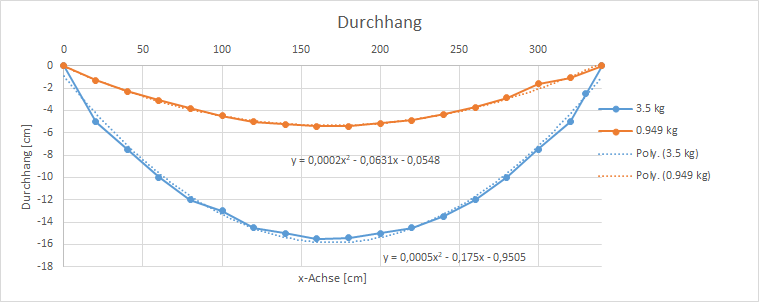
\includegraphics[width=\textwidth,keepaspectratio]{Durchhang_v1}
	\caption{Diagramm zum Durchhang}
	\label{fig:Durchhang_v1}
\end{figure}

Interessant ist, dass die tatsächlichen Werte des Durchhanges schlecht mit den errechneten Werten in Tabelle \ref{tbl:DurchhangRechnung} übereinstimmten. Dies führt daher, dass die Umlenkrollen der Plattform eine grosse Reibung aufweisen und daher die Rechnung mit konstanter Seilspannung eigentlich nicht ganz richtig ist. Die Rollen werden, jedoch von der Modulleitung noch durch Reibungsärmere ersetzt. Danach muss die Durchhangsmessung nochmals durchgeführt werden.

\subsection{Last greifen \& anheben}
\label{ssec:VersLastg}
Um die Last zu greifen fiel unsere erste Wahl ursprünglich auf eine Konstruktion mit Elektromagnet. Diesen Elektromagneten wollten wir selbst bauen. Das Testprotokoll «Elektromagnet V1» zeigt, dass die Last zwar angehoben werden konnte, der Elektromagnet jedoch sehr heiss wurde. Dies aufgrund der hohen Leistung von 4W.

Nach dem Versuch «Elektromagnet V2» wurde klar, dass durch die vorgenommenen Änderungen der Elektromagnet nur noch am Rand eine magnetische Wirkung besitzt.

Um eine Alternative ohne Elektromagnet zu testen, wurde ein Prototyp gebaut um die Teilfunktion «Last greifen» durch einen Haken umzusetzen.

%TODO Protokoll, Ergebnis, Entscheid

\subsection{Entwicklungsumgebung Informatik}
\label{ssec:VersEntI}
Ziel war es sicherzustellen, dass eine Entwicklungsumgebung zur Bilderkennung mit den bisher vorgesehenen Komponenten möglich ist. Der Versuch war erfolgreich und lieferte alle erwarteten Resultate.
Test Zielplatten Erkennung Informatik
Ziel war es, die Zielplatte mittels der Programmbibliothek OpenCV zu erkennen.
Die Zielplatte konnte grundsätzlich erkannt werden. Es stellt sich jedoch heraus, dass sobald die Lichtverhältnisse stark ändern, eine Erkennung nichtmehr möglich ist. Zudem wird die Zielplatte nicht erkannt, sobald eine der konzentrischen Bereiche / Linien durchtrennt wird. Sobald ein Hinderniss, die zu hebende Last oder Teile unseres Fahrzeuges im Weg sind, funktioniert dieser erste Prototyp der Zielplattenerkennung nicht.
Um zu wissen ob und und mit welchen Bildstörungen zu rechnen sein wird, wurde ein weitere Versuch «Kameraausrichtung» durchgeführt.

\subsection{Kameraausrichtung}
\label{ssec:VersKamera}
Ziel war es die Kameraausrichtung am Fahrzeug festzulegen und zu wissen ob und mit welchen Bildstörungen zu rechnen sein wird.
Die Kamera wird ausserhalb des Geräts angebracht um eine Überbelichtung des Sensors zu verhindern (bzw. gleichmässige Lichtverhältnisse im ganzen Bild zu erhalten).
Dieser Versuch bestätigte das Risiko, dass die Zielplatte nicht erkannt wird, sobald Störfaktoren wie Teleskoparm und/oder die Last selbst im Bild sind.  Mit der optimalen Ausrichtung der Kamera, können solche Störfaktoren vermindert, jedoch nicht komplett ausgeschlossen werden.

\subsection{Kommunikation ET - IT Board}
\label{ssec:VersKomm}
Ziel war es, die Kommunikation via UART zwischen Elektronik-Board und Informatik-Board sicherzustellen. Sie wird hauptsächlich dazu gebraucht, damit das Informatik-Board die Erkennung der Zielplatte an das steuernde Elektronik-Board weitergeben kann.


\chapter{Projektorganisation}
\label{ch:ProjektOrga}

\section{Teamübersicht}
\label{sec:Teamuebersicht}
\begin{table}[h!]
	\centering
	\begin{tabular}{|p{0.3\textwidth}|p{0.3\textwidth}|}
		\hline
		\textbf{Name} & \textbf{Studium} \\
		\hline
		Basil Bachmann & Maschinenbau \\
		\hline
		Pascal Baumann & Informatik \\
		\hline
		David Craven & Elektrotechnik \\
		\hline
		Victor Guntern & Maschinenbau \\
		\hline
		Markus Kempf & Maschinenbau \\
		\hline
		Eve Meier & Informatik \\
		\hline
		Jan Odermatt & Elektrotechnik \\
		\hline
		Simon Rohrer & Maschinenbau \\
		\hline
	\end{tabular}
	\caption{Teammitglieder}
	\label{tab:TeamMitglieder}
\end{table}

\newpage

\section{Projektrollen}
\label{sec:ProjektRollen}
\begin{table}[h!]
	\begin{tabular}{|p{0.3\textwidth}|p{0.5\textwidth}|p{0.2\textwidth}|}
		\hline
		\textbf{Rolle} & \textbf{Aufgaben} & \textbf{Teammitglied} \\
		\hline
		Projektleiter & Gesamtübersicht des Projektes halten  & Eve \\
		& Überprüfen ob Vorgaben eingehalten werden & \\
		& Teammeetings organisieren & \\
		& Informationsaustausch sicherstellen & \\
		& Kostenverwaltung & \\
		\hline
		Projektplaner & Aktualisieren des Terminplanes & Markus\\
		& Rahmenplanung und Überblick über Einhaltung Meilensteine& \\
		& Pflege Taskboard & \\
		\hline
		Verantwortlicher Dokumentation& Zusammenstellen des Abgabedokuments für Meilensteine & Pascal \\
		& Unterstützung und Pflege LaTeX &  \\
		\hline
		Protokollführer & Protokolle führen & Simon \\
		& Alte Protokolle abnehmen lassen & \\
		\hline
		Fachverantwortliche & Projektstand und Feedback & I Pascal \\
		& Ansprechperson bei Fragen & ET Jan\\
		& Aktualisierung Risikomanagement & M Markus\\
		& Koordination Versuche und Recherche & \\
		\hline
	\end{tabular}
	\caption{Rollen in unserem Team}
	\label{tab:Projektrollen}
\end{table}

\section{Tools}
\label{sec:Tools}
\begin{table}[h!]
	\begin{tabular}{|p{0.4\textwidth}|p{0.6\textwidth}|}
		\hline
		\textbf{Aufgabe} & \textbf{Hilfsmittel} \\
		\hline
		Dokumente und Dokumentation & LaTeX / MiKTeX / GitHub \\
		\hline
		Quellen & Mendeley \\
		\hline
		Dateiablage für Teamaustausch & Dropbox \\
		\hline
		Dateiablage für Abgabe & Ilias \\
		\hline
		Projekt- und Budgetplan & MS Excel 2016 \\
		\hline
		Kommunikation Team & WhatsApp Gruppe oder über die HSLU Mailadresse\\
		\hline
		Aufgabenverwaltung & SCRUM-angelehntes Board, physisch, Teaminsel\\
		\hline
	\end{tabular}
	\caption{Softwaretools}
	\label{tab:SWTools}
\end{table}

\newpage

\section{Wochenplan}
\label{sec:Wochenplan}
\begin{table}[h!]
	\begin{tabular}{|p{0.2\textwidth}|p{0.8\textwidth}|}
		\hline
		\textbf{Tag} & \textbf{Beschreibung} \\
		\hline
		DO 08:30 & Alle Mitglieder sind in der Teaminsel \\
		\hline
		DO 08:30-09:00 & Besprechung Team-intern erledigte Aufgaben \\
		& Fragen, weiteres Vorgehen \\
		\hline
		DO 09:00-10:00 & Arbeiten im Team od. selbständig \\
		\hline
		DO 10:00-10:20 & Pause \\
		\hline
		DO 10:20-12:00 & Arbeiten im Team od. selbstständig \\
		\hline
		FR 08:30 & Alle Mitglieder sind in der Teaminsel \\
		\hline
		FR 08:30-09:00 & Besprechung Team-intern, Vorbereitung Meeting mit Dozent \\
		\hline
		FR 09:00-09:30& Besprechung mit Dozent \\
		\hline
		FR 09:30-10:00 & Arbeiten im Team od. selbstständig \\
		\hline
		FR 10:00-10:20 & Pause \\
		\hline
		FR 10:20-11:00 & Arbeiten im Team od. selbstständig \\
		\hline
		FR 11:00-11:30 & Kurzbesprechung, Taskboard aktualisieren \\
		\hline
		FR 11:30-12:00 & Arbeiten im Team oder selbstständig (freiwillig)\\
		\hline
	\end{tabular}
	\caption{Wochenplan}
	\label{tab:Wochenplan}
\end{table}


\section{Projektplan}
\label{sec:Projektplan}
An dieser Stelle ist der Projektplan grob umrissen, den Detaillierten finden Sie im Anhang.

\begin{figure}[h!]
	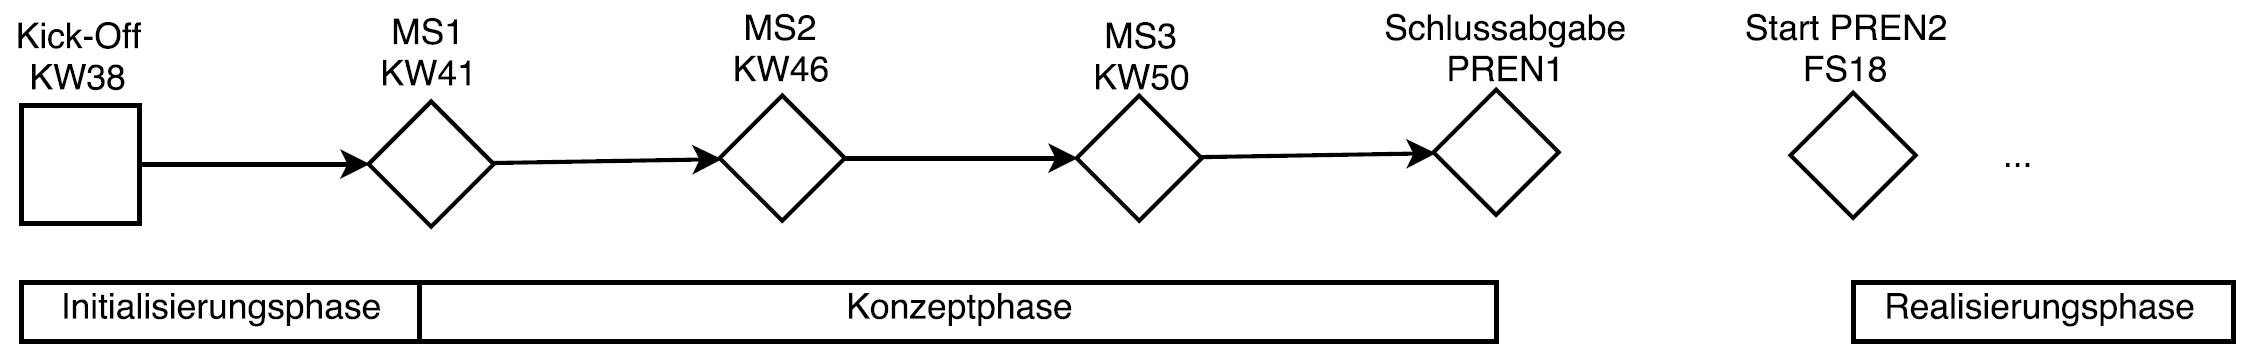
\includegraphics[width=\linewidth,keepaspectratio]{Rahmenplan}
	\caption{Grober Projektplan}
	\label{fig:GrobProjekt}
\end{figure}

\begin{table}[h!]
\vspace{1em}
\noindent
\begin{tabular}{|p{0.2\textwidth}|p{0.2\textwidth}|p{0.55\textwidth}|}
	\hline
	\textbf{Meileinstein} & \textbf{Termin} & \textbf{Beschreibung} \\
	\hline
	Start & 21.09.2017 & Input 1 mit Einfürung \\
	\hline
	Meilenstein 1 & 13.10.2017 12:00 Uhr & Projektorganisation, Technologierecherche, Anforderungsliste \\
	\hline
	Meilenstein 2 & 10.11.2017 12:00 Uhr & Risikomanagement, Evaluation der Lösungsprinzipien und Auswahl der optimalen Lösungskombination(en) \\
	\hline
	Meilenstein 3 & 15.12.2017 12:00 Uhr & Freigabe des Gesamtkonzepts, Dokumentation zu 80\% fertig gestellt. \\
	\hline
	Schlussabgabe PREN1 &12.01.2018 & Schlussabgabe Dokumentation zu 100\% fertig \\
	\hline
	\end{tabular}
	\caption{Meilensteine}
	\label{tab:Meilensteine}
\end{table}

\newpage

\section{Budgetplan}
\label{sec:Budgetplan}
Für den Bau der Teilfunktionsmuster in PREN1 dürfen maximal CHF 200.- ausgegeben werden. Die Tabelle \ref{tab:Budgetplan} dient daher vor allem der Kostenverfolgung, damit das Budget nicht überzogen wird.

\vspace{1em}
\noindent
\begin{table}[h]
	\begin{tabular}{|p{0.3\textwidth}|p{0.15\textwidth}|p{0.225\textwidth}||p{0.225\textwidth}|}
	\hline
	\textbf{Artikel} & \textbf{Anzahl} & \textbf{Preis/Stk. CHF} & \textbf{Total CHF} \\
	\hline
	Rillenkugellager 608-2RS & 2 & 8.36 & 16.72 \\
	\hline
	Sinterbronzebuchse PSM 050810 & 5 & 3.78 & 18.9 \\
	\hline
	Rundstab Buche & 3 & 0.9 & 2.7 \\
	\hline
	Buche Rundstäbe glatt & 1 & 0.7 & 0.7 \\
	\hline
	HDF 1200x500x3mm (Holzplatte) & 1 & 5.4 & 5.4 \\
	\hline
	Aluminium Rohmaterial & 1 & 10 & 10 \\
	\hline
	Kabel Set (ca. 40 Stück) - female/female & 1 & 9.9 & 9.9 \\
	\hline
	Original Raspberry Pi Kamera Module V2 & 1 & 29.9 & 29.9 \\
	\hline
	Raspberry Pi Model B & 1 & 25.5 & 25.5 \\
	\hline
	Lofive & 1 & 25 & 25 \\
	\hline
	LSM6DS3 Breakout & 1 & 13.4 & 13.4 \\
	\hline
	TURNIGY 1800MAH 3S 20C LIPO-PACK & 1 & 25 & 25\\
	\hline
	\textbf{Total} & & & \textbf{183.12} \\
	\hline
	\end{tabular}
	\caption{Budgetplan für das Projekt im PREN01}
	\label{tab:Budgetplan}
\end{table}

\chapter{Risikomanagement}
\label{ch:RisikoMgmt}
In diesem Kapitel werden mögliche Risiken während des Projektverlaufes aufgelistet. Dabei werden Projektrisiken nummeriert. Ihre Eintrittswahrscheinlichkeit und ihr Schadensausmass wird eingeschätzt. Besteht ein grosses Risiko, werden zusätzlich Massnahmen definiert.

\section{Definitionen}
\label{sec:Def}
\vspace{1em}
\noindent
Eintrittswahrscheinlichkeit:

\vspace{1em}
\noindent
\begin{tabular}{|p{0.06\textwidth}|p{0.2\textwidth}|p{0.7\textwidth}|}
	\hline
	\textbf{Stufe} & \textbf{Bezeichnung} & \textbf{Beschreibung} \\
	\hline
	1 & unvorstellbar & Möglich aber eher unwahrscheinlich. Tritt nie oder einmal in 14 Wochen auf \\
	\hline
	2 & unwahrscheinlich & Kann in 14 Wochen 1-5 Mal eintreten\\
	\hline
	3 & vorstellbar & Kann in 14 Wochen 6-8 Mal eintreten \\
	\hline
	4 & wahrscheinlich & Kann in 14 Wochen bis zu 10 Mal eintreten \\
	\hline
	5 & häufig & Kann in 14 Wochen 14 Mal eintreten\\
	\hline
\end{tabular}

\vspace{1em}
\noindent
Schadensausmass:

\vspace{1em}
\noindent
\begin{tabular}{|p{0.06\textwidth}|p{0.2\textwidth}|p{0.7\textwidth}|}
	\hline
	\textbf{Stufe} & \textbf{Bezeichnung} & \textbf{Beschreibung} \\
	\hline
	1 & unwesentlich & Die Aufgabenerfüllung wird höchstens geringfügig beeinträchtigt finanzieller Schaden ist im Rahmen des Projekts nicht beeinflussend. Personenschäden treten nicht auf \\
	\hline
	2 & geringfügig & Wahrnehmbare Gefährdung / Einfluss auf das Projekt. Personenschäden treten nicht auf \\
	\hline
	3 & mittelmässig & Wahrnehmbare Gefährdung / Einfluss auf das Projekt.Finanzieller Schaden strapaziert das Projektbudget
	Personenschäden treten nicht auf \\
	\hline
	4 & kritisch & Starke Gefährdung des Projekts. Finanzieller Schaden übersteigt das Projektbudget massiv. Personenschäden treten geringfügig auf \\
	\hline
	5 & katastrophal & Projektabbruch zur Folge. Finanzieller Schaden kann zum Projektstopp führen. Verletzung der Persönlichkeitsrechte
	\\
	\hline
\end{tabular}


\section{Risikokatalog}
\label{sec:Risikokatalog}
Legende:
\begin{itemize}
	\item \textbf{S}chadensausmass bei Eintreffen des Risikos
	\item \textbf{W}ahrscheinlichkeit das Risiko eintrifft
	\item \textbf{K}ategorie: \textbf{T}echnisches oder \textbf{P}rojektbezogenes Risiko
	\item \textbf{A}uswirkung auf das Projekt. Produkt aus S und W
\end{itemize}

\vspace{1em}
\noindent
\begin{tabular}{|p{0.03\textwidth}|p{0.75\textwidth}|p{0.03\textwidth}|p{0.03\textwidth}|p{0.03\textwidth}||p{0.03\textwidth}|}
	\hline
	\textbf{Nr.} & \textbf{Beschreibung / Risiko} & \textbf{K} & \textbf{S} & \textbf{W} & \textbf{A} \\
	\hline
	1 & Datenverlust & P & 5 & 1 & 5\\
	\hline
	2 & Zerstörung elektronischer Komponenten durch ESD & T & 3 & 3 & 9 \\
	\hline
	3 & Störung der Steuerungskomponenten durch Elektromotoren & T & 3 & 2 & 6 \\
	\hline
	4 & Fortbewegungsschwierigkeiten des Gerätes & T & 5 & 2 & 10 \\
	\hline
	5 & Schwankungen des Gerätes & T & 2 & 3 & 6 \\
	\hline
	6 & Probleme beim Transport der Last & T & 4 & 2 & 8 \\
	\hline
	7 & Probleme Fertigung oder Beschaffung Komponenten & P & 2 & 3 & 6 \\
	\hline
	8 & Stop über Zielplatzform schlägt fehl & T & 4 & 2 & 8 \\
	\hline
	9 & Fehlkommunikation im Team & P & 3 & 3 & 9 \\
	\hline
	10 & Teammitglied fällt aus & P & 3 & 2 & 6 \\
	\hline
	11 & Verzug bei Erstellung von Dokumenten & P & 3 & 2 & 6 \\
	\hline
	12 & Gerät startet nicht & T & 5 & 1 & 5 \\
	\hline
\end{tabular}

\section{Risikobewertung}
\label{sec:RisikoBewertung}
\begin{figure}[h!]
	\centering
	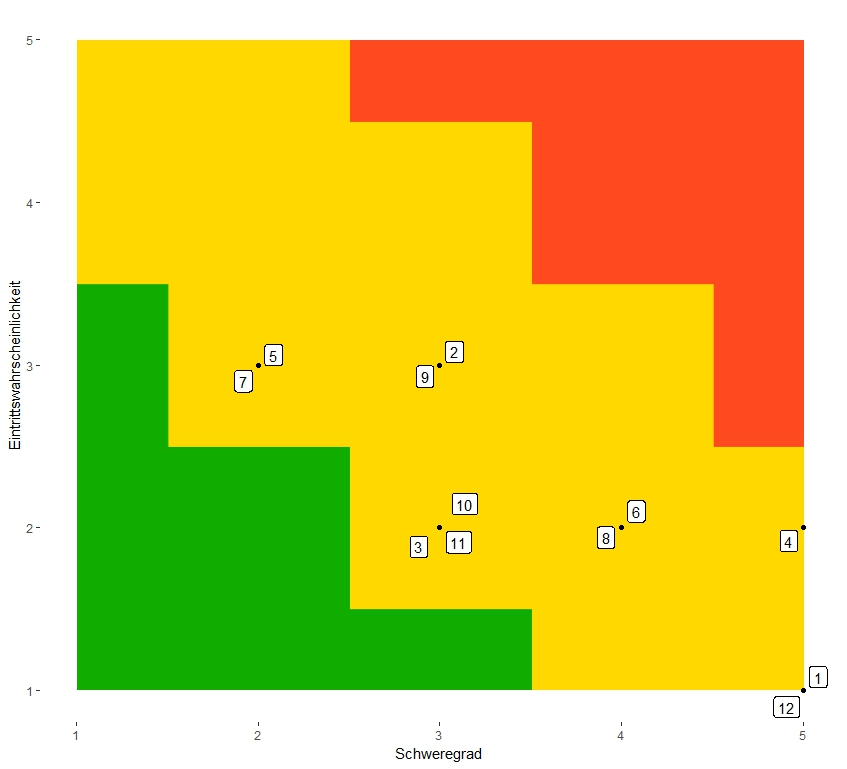
\includegraphics[width=.6\textwidth,keepaspectratio]{Risikomatrix}
	\caption{Die Risiken aus dem Risikokatalog graphisch dargestellt}
	\label{fig:Risikomatrix}
\end{figure}

\section{Massnahmen}
\label{sec:Massnahmen}
\vspace{1em}
\noindent
\begin{table}[h!]
	\centering
	\begin{tabular}{|p{0.1\textwidth}|p{0.9\textwidth}|}
		\hline
		\textbf{Risiko Nr.} & \textbf{Massnahme} \\
		\hline
		1 & Es wird sowohl für Dokumentation und Programmcode mit GitHub als Versionskontrollsystem gearbeitet. Sonstige Daten befinden sich in der Dropbox. Dropbox wird als sicher eingestuft. \\
		\hline
		2 & Gesamtes Team ist im Umgang mit elektronischen Komponenten geschult. \\
		\hline
		3 & Magnetische Abschirmung des Elektromotors ist vorgesehen. Klare Aufteilung der Printplatte in Digital und Analog. \\
		\hline
		4 & Grösst mögliche Steigung des Seiles wird miteinbezogen. Laufkatze wird gegen rutschen und abstürzen gesichert. Akkuleistung wird genügend gross gewählt. \\
		\hline
		5 & Stabilisierung des Gerätes durch Gewicht oder Dämpfer. \\
		\hline
		6 & Erkennen, greifen und absetzen der Last muss durch Tests in 9 von 10 Mal funktionieren. \\
		\hline
		7 & Aufträge werden frühzeitig in Auftrag gegeben. Vor Auftragserteilung und Bestellung werden diese durch mindestens zwei Personen Überprüft.\\
		\hline
		8 & Zielerkennung wird unter verschiedenen Bedingungen (zum Beispiel Lichteinflüssen) getestet und muss in 9 von 10 Mal funktionieren. Laufkatze soll vor- und rückwärts fahren können. \\
		\hline
		9 & Bei Unklarheiten und Unwohlsein wird von jedem Teammitglied erwartet, dass er sich selbst meldet. Zur Veranschaulichung technischer Aspekte wird mit Skizzen gearbeitet. \\
		\hline
		10 & Aktueller Stand ist zu jedem Zeitpunkt allen klar. Aufgaben-Board ist immer aktuell. Im Falle eines Teammitgliedsausfall kann so jemand anderes übernehmen. \\
		\hline
		11 & Mit Arbeiten und dazugehöriger Dokumentation wird frühzeitig begonnen. Der Aufwand wird grosszügig mit einberechnet / Puffer. \\
		\hline
		12 & Aufbau der Laufkatze wird geübt und soll nie länger als 1.5min dauern. Das Startsignal soll über zwei Verschiedenen Kanäle gesendet werden können. \\
		\hline
	\end{tabular}
	\caption{Massnahmen welche definiert wurden um die Risiken aus \ref{sec:Risikokatalog} zu minimieren}
	\label{tab:Massnahmen}
\end{table}

\newpage
\subsection{Effekt der Massnahmen}
\label{ssec:MassEffekt}
\begin{figure}[h!]
	\centering
	\begin{subfigure}[b]{0.45\textwidth}
		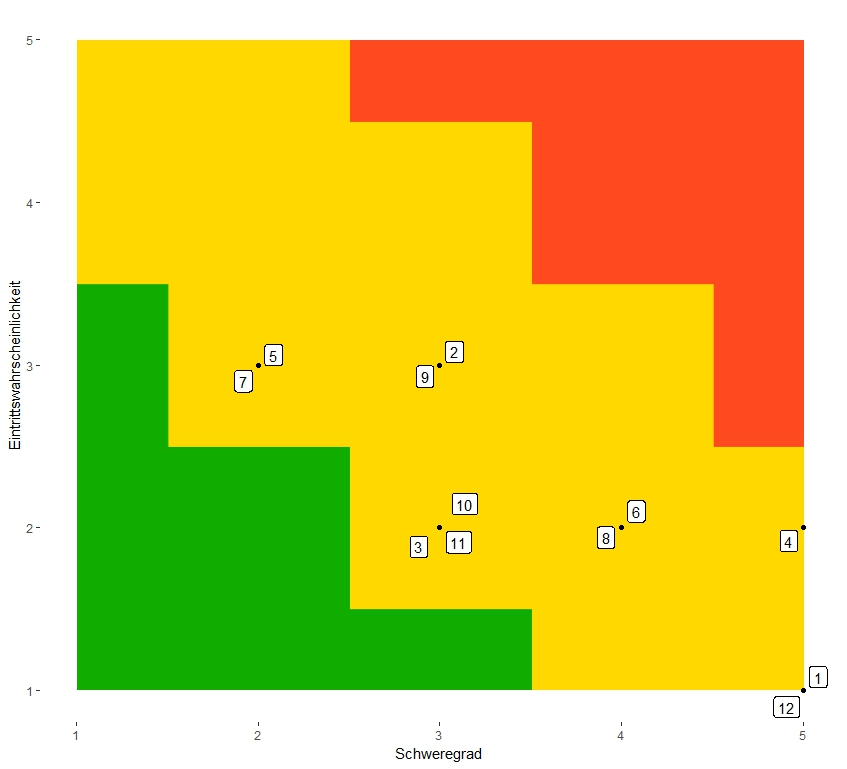
\includegraphics[keepaspectratio,width=\textwidth]{Risikomatrix}
	\end{subfigure}
	\begin{subfigure}[b]{0.45\textwidth}
		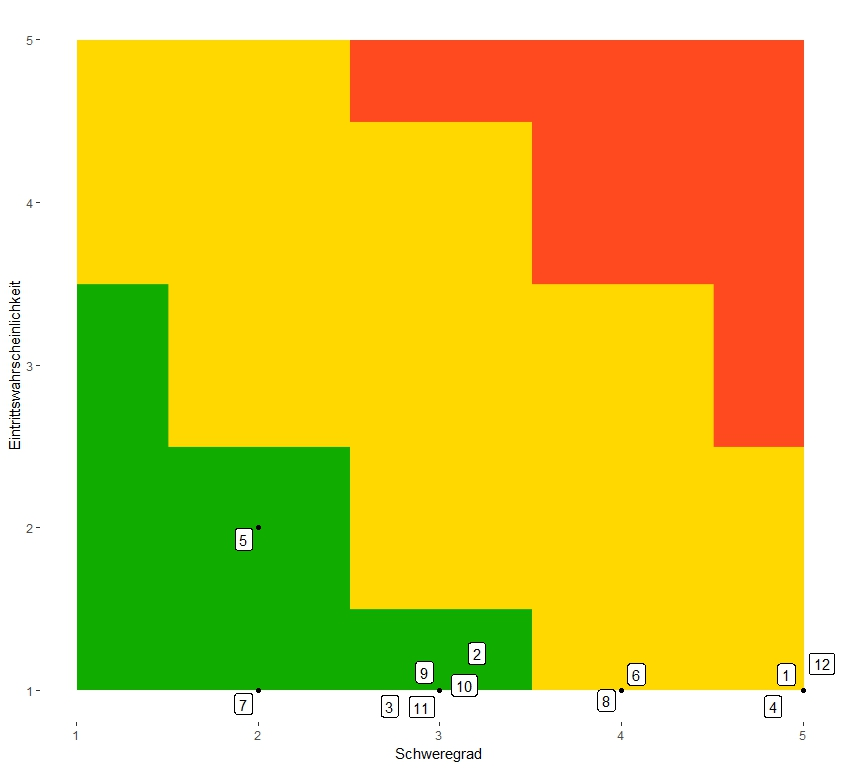
\includegraphics[keepaspectratio,width=\textwidth]{Risikomatrix_nachher}
	\end{subfigure}
	\caption{Gegenüberstellung der Risikomatrizen vor und nach den Massnahmen}
	\label{fig:Gegenueberstellung}
\end{figure}

\begin{figure}[h!]
	\centering
	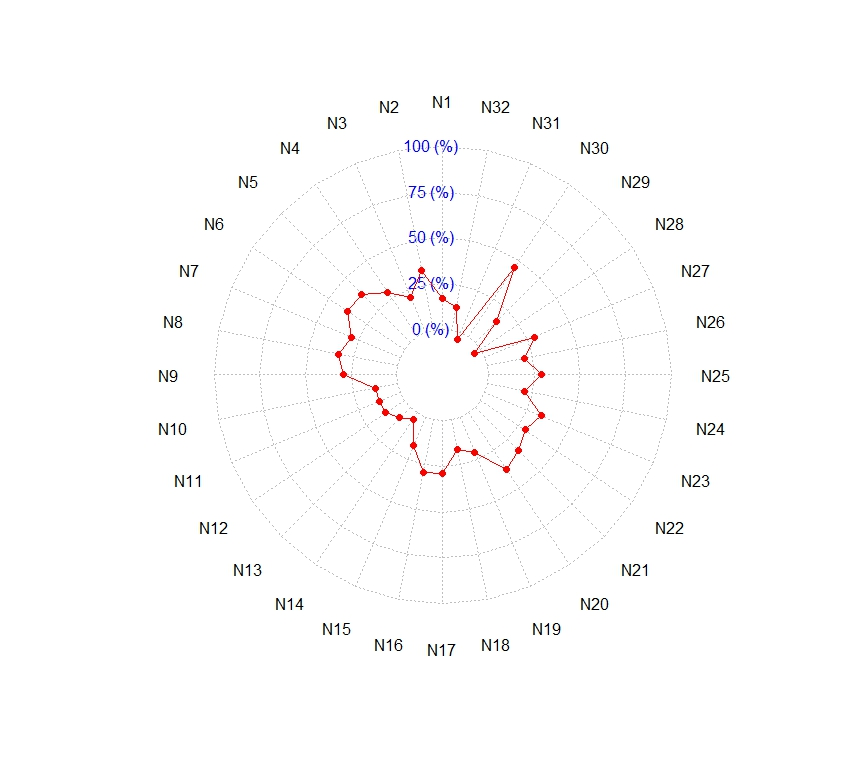
\includegraphics[width=\textwidth,keepaspectratio]{Risikomatrix_Spinne}
	\caption{Die Risiken aus dem Risikokatalog graphisch dargestellt, die rote Linie zeigt die Risiken vor den Massnahmen, während die Grüne die Risiken nach dem Anwenden der Massnahmen darstellt}
	\label{fig:Risikomatrix_Spinne}
\end{figure}

\chapter{Schlussdiskussion}
\label{ch:SchlussDisku}
\listoffigures

\listoftables

\printbibliography

\appendix

\chapter{Aufgabenstellung im Original}
\label{app:ch:AufgabenOriginal}
Die Aufgabenstellung im Original folgt auf den nächsten Seiten.

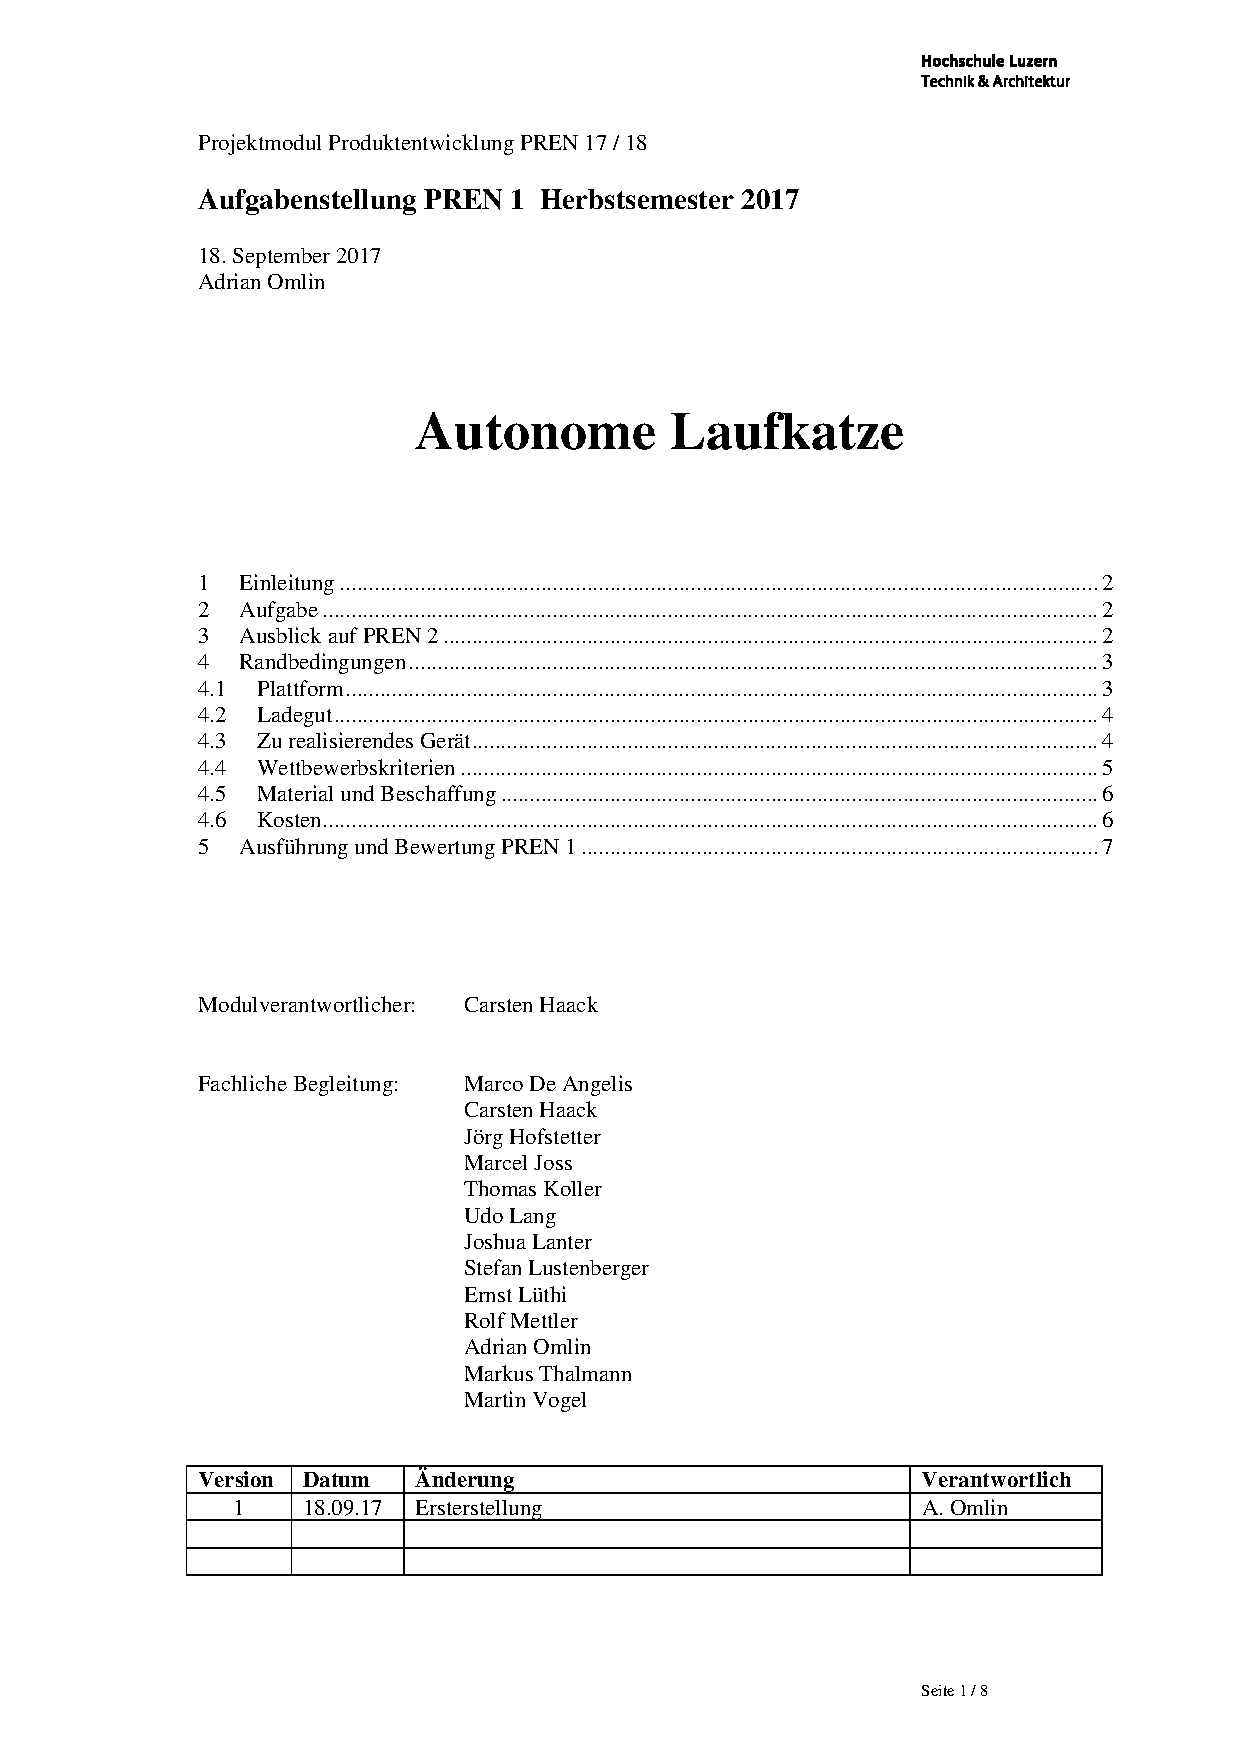
\includepdf[pages=1-8]{AufgabenstellungPREN1H17.pdf}

\chapter{Anforderungen}
\label{app:ch:Anforderungen}
\section{Projektanforderungen}
\label{app:sec:ProjektAnf}
\begin{tabular}{|p{.05\textwidth}|p{0.07\textwidth}|p{0.3\textwidth}|p{0.55\textwidth}|}
	\hline
	\textbf{Nr.} & \textbf{FMW\footnotemark} & \textbf{Bezeichnung} & \textbf{Beschreibung} \\
	\hline
	1.1 & F & Projektabgabe & Dezember 2017 \\
	\hline
	1.2 & F & Eigenleistung & Systemkomponenten können zugekauft werden \\
	\hline
	1.3 & F & Interdisziplinarität & Disziplinen / Abteilungen arbeiten zusammen \\
	\hline
	1.4 & W & Lieferantenwahl & Für Sammelbestellungen gem. Kapitel 4.5 der Aufgabenstellung. Wird Material vom Team selbst gekauft, können die Kosten zurückgefordert werden \\
	\hline
	1.5 & M & Budget f. PREN & max. 500.- CHF \\
	\hline
	1.6 & M & Teilbudget PREN1 & max. 200.- CHF \\
	\hline
	1.7 & M & 3D-Drucker Laufzeit & max. 25h \\
	\hline
	1.8 & M & Lasergerät Laufzeit & max. 1h \\
	\hline
	1.9 & M & Stunden ET-Werkstattpersonal & max. 10h \\
	\hline
	1.10 & M & Stunden M-Werkstattpersonal & max. 10h \\
	\hline
	1.11 & F & "Gesponsorte"\ Komponenten & Werden mit einem realistischen Preis in die Kostenrechnung einbezogen \\
	\hline
\end{tabular}
\footnotetext{F: Festanforderung M: Mindestanforderung W: Wunschanforderung }

\section{Plattform}
\label{app:sec:Plattform}
\begin{tabular}{|p{.05\textwidth}|p{0.07\textwidth}|p{0.3\textwidth}|p{0.55\textwidth}|}
	\hline
	\textbf{Nr.} & \textbf{FMW\footnotemark} & \textbf{Bezeichnung} & \textbf{Beschreibung} \\
	\hline
	2.1 & F & Gesamtlänge & 350 $\pm$ 2cm \\
	\hline
	2.2 & F & Masten Abstand & Abstand zwischen den Masten 350cm $\pm$ 2cm \\
	\hline
	2.3 & F & Masten Masse & 8cm Front, 6cm Tiefe \\
	\hline
	2.4 & F & Drahtseil & Verzinkter Stahl, Durchmesser 3mm \\
	\hline
	2.5 & F & Seilspannung & Via Umlenkrollen durch ein Gewicht mit einer Masse von 15kg \\
	\hline
	%TODO Winkel des Seiles
	2.6 & F & Winkel des Seiles & \\
	\hline
	2.7 & F & Grundplatte & Spanplatte roh oder grau gestrichen.\\
	& & & Mit Farbresten / vorstehenden Schrauben und Nahtstellen ist zu rechnen \\
	\hline
	2.8 & F & Startfeld & 50cm $\pm$ 2cm, Quadratisch \\
	\hline
	2.9 & F & Zielplatte & TODO Gesamtmass? \\
	\hline
	2.10 & F & Zielplatte Aussehen & 5 konzentrische Bereiche?\\
	& & & Der innerste, helle Bereich ist quadratisch und hat eine Seitenlänge von 6cm $\pm$ 2mm. \\
	& & & Jeder daran anschliessende konzentrische Bereich hat eine Breite von 2.5cm $\pm$ 2mm. \\
	& & & Die Bereiche sind abwechslungsweise hell und dunkel \\
	\hline
	2.11 & F & Zielplatte Position & Der Absetzbereich verläuft unterhalb des Seiles und ist 2cm breit.\\
	& & & Die Zielplatte kann bis zum Startsignal verschoben werden.\\
	& & & Befindet sich aber immer im Absetzbereich (siehe Abbildung 1 der Aufgabenstellung) \\
	\hline
	2.12 & F & Start- und Zielplatte & Matt \\
	\hline
	2.13 & F & Hindernisse & Auf der gesamten Plattform können Hindernisse stehen.\\
	& & & Im Umkreis von mindestens 10cm um die Startposition des Ladegutes und um die Zielplatte herum sind keine Hindernisse \\
	\hline
	2.14 & M & Hindernisse Höhe & Die Hindernisse haben eine maximale Höhe von 20cm. \\
	\hline
\end{tabular}
\footnotetext{F: Festanforderung M: Mindestanforderung W: Wunschanforderung }

\section{Laufkatze}
\label{app:sec:LaufKatze}
\begin{tabular}{|p{.05\textwidth}|p{0.07\textwidth}|p{0.3\textwidth}|p{0.55\textwidth}|}
	\hline
	\textbf{Nr.} & \textbf{FMW\footnotemark} & \textbf{Bezeichnung} & \textbf{Beschreibung} \\
	\hline
	3.1 & F & Steuerung & Autonom \\
	\hline
	3.2 & M & Inbetriebnahme & Darf max. 2min dauern \\
	\hline
	3.3 & M & Startsignal & Darf per Kopfdruck gesendet werden \\
	\hline
	3.4 & M & Geschwindigkeit & Um die Aufgabe zu bewältigen steht der Laufkatze\\
	& & & ein Zeitfensters von 4min zur Verfügung. \\
	\hline
	3.5 & M & Aussendimensionen & Die Laufkatze darf in ihrer Projektion das Startfeld nicht überschreiten. 50cm $\pm$ 2cm x 50cm $\pm$ 2cm \\
	\hline
	3.6 & F & Bauart & Sämtliche Sensorik muss auf dem Gerät selbst montiert sein. \\
	\hline
	3.7 & F & Fahrweise & Das Gerät darf nur das Drahtseil und den zweiten Masten berühren.\\
	& & & Die gesamte Plattform, insbesondere Drahtseil, die Last und die Zielplatte dürfen nicht beschädigt oder sonst irgendwie verändert werden.\\
	& & & Es ist beispielsweise nicht erlaubt, Navigationshilfen anzubringen. \\
	\hline
	3.8 & F & Ladegut & Das Gerät muss ein Ladegut transportieren können. \\
	\hline
	3.9 & F & Zielerkennung & Das Erkennen der Zielplatte muss selbstständig erfolgen\\
	\hline
\end{tabular}
\footnotetext{F: Festanforderung M: Mindestanforderung W: Wunschanforderung }

\section{Ladegut}
\label{app:sec:AnfLadegut}
\begin{tabular}{|p{.05\textwidth}|p{0.07\textwidth}|p{0.3\textwidth}|p{0.55\textwidth}|}
	\hline
	\textbf{Nr.} & \textbf{FMW\footnotemark} & \textbf{Bezeichnung} & \textbf{Beschreibung} \\
	\hline
	4.1 & F & Material & Holz \\
	\hline
	4.2 & F &  Dimensionen & Seitenlänge 5cm $\pm$ 0.5cm \\
	\hline
	4.3 & M & Gewicht & 50-90g, siehe Sektion \ref{app:sec:RechKlotzMasse} \\
	\hline
	4.4 & F & Aufnahme & Metallischer, magnetischer Hacken oben in der Mitte des Würfels.\\
	& & & Innendurchmesser des Hakens ist 1.3cm $\pm$ 0.1mm\\
	\hline
	4.5 & F & Hindernisse & Das Ladegut darf Hindernisse nicht berühren. \\
	\hline
	4.6 & F & Position & Die Position des Ladegutes muss in Echtzeit angezeigt werden, dass der Schiedsrichter jederzeit die angezeigten Werte gut erkennen kann.\\
	& & & TODO auf Gerät od. Extern? \\
	\hline
	4.7 & F & Positionsbestimmung & Die Mitte des Bodens des Ladegutes wird verwendet.\\
	& & & Die Position muss in x- und z-Richtung bestimmt werden (siehe Skizze Anforderungen).\\
	& & & Der Nullpunkt des zu verwendenden Koordinatensystems ist in Abbildung 1 der Aufgabenstellung definiert. \\
	\hline
	4.8 & F & Absetzen & Das Ladegut muss innerhalb des Zielbereiches automatisch abgesetzt werden. \\
	\hline
	4.9 & F & Zielbereich & Der Zielbereich muss automatisch erkennt werden\\
	\hline
\end{tabular}
\footnotetext{F: Festanforderung M: Mindestanforderung W: Wunschanforderung }

\section{Umfeld}
\label{app:sec:Umfeld}
\begin{tabular}{|p{.05\textwidth}|p{0.07\textwidth}|p{0.3\textwidth}|p{0.55\textwidth}|}
	\hline
	\textbf{Nr.} & \textbf{FMW\footnotemark} & \textbf{Bezeichnung} & \textbf{Beschreibung} \\
	\hline
	5.1 & M & Licht & Scheinwerfer welche auf die Wettbewerbsplattformen gerichtet sind, werden dazu führen, dass wir mit einer hohen Helligkeit arbeiten müssen \\
	\hline
	5.2 & M & Temperaturen & Bei Lagerung und Betrieb Zimmertemperatur 15-\SI{20}{\degreeCelsius}\\
	\hline
	5.3 & M & Kein Spritzwasser & Für Innenanwendung\\
	\hline
	5.4 & M & Keine Hochspannung & Normale Netzspannung\\
	\hline
	5.5 & M & Raumhöhe & Als Wettbewerbsraum wird eine Normale Raumhöhe (2.5-3m) angenommen.\\
	\hline
\end{tabular}
\footnotetext{F: Festanforderung M: Mindestanforderung W: Wunschanforderung }

\chapter{Technologierecherche}
\label{app:ch:TechRech}
Bevor wir mit unserer, eigenständigen Recherche begannen, sassen wir im Team zusammen und machten ein Brainstorming. Dabei kamen wir auf die folgenden Ideen:

\begin{multicols}{2}
\paragraph{Plattformen}
\begin{itemize}[noitemsep]
	\item Raspberry Pi
	\item Arduino
	\item Hifive
\end{itemize}

\paragraph{Programmierprache}
\begin{itemize}[noitemsep]
	\item Python
	\item Java
	\item C\#
	\item Rust
\end{itemize}

\paragraph{Bilderkennung}
\begin{itemize}[noitemsep]
	\item OpenCV
	\item ImageJ
	\item Eigener Algorithmus
\end{itemize}

\paragraph{Position, Last bestimmen \& darstellen}
\begin{itemize}[noitemsep]
	\item 2x 7-Segment
	\item Echolot
	\item Time of Flight
	\item Drehgeber
	\item z-Position
	\item Schrittmotor
	\item LCD
	\item OLED
	\item Bluetooth
\end{itemize}

\paragraph{Zielzone erkennen}
\begin{itemize}[noitemsep]
	\item Kamera
	\item Sensoren
	\item Beleuchtung
\end{itemize}

\paragraph{Startsignal}
\begin{itemize}[noitemsep]
	\item Bluetooth
	\item Knopf
	\item WiFi
	\item Akustisch
\end{itemize}

\paragraph{Energieversorgung}
\begin{itemize}[noitemsep]
	\item Eingebauter Akku
	\item Battery Pack
	\item Li-Ion
	\item NiCad
	\item Supercapacitor (SC)
	\item Bleiakku
	\item Solarpanel
	\item Verbrennungsmotor
	\item Dieselgenerator
	\item Brennstoffzelle
\end{itemize}

\paragraph{Stabilisierung}
\begin{itemize}[noitemsep]
	\item Federn \& Dämpfen
	\item Gyroskop
	\item Tank/Flüssigkeit hin-und herpumpen
	\item Rotoren
	\item Ausgleichsdüsen
\end{itemize}

\paragraph{Antrieb}
\begin{itemize}[noitemsep]
	\item Magnetschwebe
	\item Zeppelin \& Ventilator
	\item Rollen eingeklemmt am Seil
	\item Seilbahn
\end{itemize}

\paragraph{Last anheben/senken}
\begin{itemize}[noitemsep]
	\item Seil
	\item Zahnstange
	\item Teleskoparm
	\item Abwerfen
\end{itemize}
\vspace{2em}
\paragraph{Aufhängung}
\begin{itemize}[noitemsep]
	\item \textquotedblleft Obe druff\textquotedblright
	\item \textquotedblleft Une ane\textquotedblright
	\item Gelenkig \& gedämpft
	\item Heliumballon
\end{itemize}

\paragraph{Last greifen}
\begin{itemize}[noitemsep]
	\item Haken
	\item Saugnapf
	\item Greifer
	\item (Elektro)Magnet
	\item Permanentmagnet
	\item Kranarm
\end{itemize}
\end{multicols}

\subsection{Recherchenbewertung}
\label{app:ssec:RechBew}
Die jeweiligen Quellen werden nach folgendem Schema bewertet:
\begin{itemize}
	\item \textbf{U}mfang (0-5)
	\item \textbf{N}utzen (0-5)
	\item \textbf{B}ewertung = Nutzen + Umfang
\end{itemize}

\vspace{1em}
\noindent
\begin{tabular}{|p{0.3\textwidth}|p{0.02\textwidth}|p{0.02\textwidth}|p{0.02\textwidth}|p{0.5\textwidth}|}
	\hline
	\textbf{Beschreibung} & \textbf{U} & \textbf{N} & \textbf{B} & \textbf{Quelle} \\
	\hline
	Beschreibung der Quelle in Stichworten & 3 & 3 & 6 & [LINK]\\
	\hline
\end{tabular}

\section{Plattformen}
\label{app:sec:Plattformen}
\subsection{Informatik}
\label{app:ssec:Inf}
\vspace{1em}
\noindent
\begin{tabular}{|p{0.3\textwidth}|p{0.02\textwidth}|p{0.02\textwidth}|p{0.02\textwidth}|p{0.5\textwidth}|}
	\hline
	\textbf{Beschreibung} & \textbf{U} & \textbf{N} & \textbf{B} & \textbf{Quelle} \\
	\hline
	TinkerBoard & 3 & 3 & 6 & https://goo.gl/tBE2uP\\
	\hline
	Raspberry Pi 3 Model B & 1 & 3 & 4 & https://goo.gl/zV2NYF \\
	\hline
	Banana PI M2 Berry & 2 & 3 & 5 & http://www.banana-pi.org/m2ub.html \\
	\hline
	BeagleBone Black Rev & 1 & 2 & 3 & https://beagleboard.org/black/\\
	\hline
	RasPi vs TinkerBoard & 3 & 3 & 6 & https://goo.gl/UeD7um\\
	\hline
	RasPi vs TinkerBoard & 1 & 3 & 4 & https://goo.gl/a3ucY6\\
	\hline
	RasPi vs BananaPi & 2 & 3 & 5 & https://goo.gl/F4eXrp\\
	\hline
	RasPi vs BananaPi & 3 & 5 & 8 & https://goo.gl/JRHX78\\
	\hline
\end{tabular}

\vspace{1em}
Sowohl bei dem Raspberry Pi als auch beim Tinkerboard sind WLAN und Bluetooth
Schnittstellen inbegriffen. Zum benutzen von OpenCV ist eine MMU und eine FPU
notwendig. Deshalb kommen nur Boards in Frage die einen ARM Cortex-A Prozessor
haben. Da aber das TinkerBoard eher dürftige Dokumentation und Unterstützung von Software besitzt \parencite[Fazit]{Finnamore2017} bevorzugen wir das Raspberry Pi.

\subsection{Elektrotechnik}
\label{app:ssec:ET}
\subsubsection{Quellen}
\begin{tabular}{|p{0.3\textwidth}|p{0.02\textwidth}|p{0.02\textwidth}|p{0.02\textwidth}|p{0.5\textwidth}|}
	\hline
	\textbf{Beschreibung} & \textbf{U} & \textbf{N} & \textbf{B} & \textbf{Quelle} \\
	\hline
	Hi-/LoFive Kurzbeschreibung & 2 & 2 & 4 & http://alturl.com/b7zyd \\
	\hline
	SiFive Controller Manual \& Cons & 5 & 4 & 9 & http://alturl.com/objsw \\
	\hline
	SiFive Datasheet & 3 & 5  & 8 & http://alturl.com/7t4ya \\
	\hline
	SiFive userlevel ISA & 5 & 3 & 8 & http://alturl.com/9rvz6 \\
	\hline
\end{tabular}

\vspace{1em}
\noindent
\begin{tabular}{|p{0.3\textwidth}|p{0.33\textwidth}|p{0.3\textwidth}|}
  \hline
  \textbf{Name} & \textbf{Vorteile} & \textbf{Nachteile} \\
  \hline
	Arduino Uno R3 & Hoher Verbreitungsgrad, viel bestehende Software & 8-bit MCU \\
	\hline
  Lofive & Hat einen RV32IMAC Prozessor, verwendet einen externen Programmierer, ist die Abgespeckte version vom Hifive Board das besser für die Integration in ein Produkt geeignet ist & Keine \\
  \hline
  Hifive & Hat einen RV32IMAC Prozessor, ist Pin-Kompatibel mit Arduino & Hat die Hardware für die Programmierung auf dem Board \\
  \hline
\end{tabular}
\section{Programmiersprache}
\label{app:sec:PrgSprachen}

\subsection{Informatik}
\label{app:ssec:PrgInf}
Die nachfolgende Recherche wurde unter der Annahme gemacht, dass wir in der Informatik das Raspberry Pi (nachfolgend RasPi genannt) als Plattform benutzen werden. Generell sollte aber Vor- und Nachteile der Sprachen universell sein.

\vspace{1em}
\noindent
\begin{tabular}{|p{0.3\textwidth}|p{0.02\textwidth}|p{0.02\textwidth}|p{0.02\textwidth}|p{0.5\textwidth}|}
	\hline
	\textbf{Beschreibung} & \textbf{U} & \textbf{N} & \textbf{B} & \textbf{Quelle} \\
	\hline
	RasPi untersützte Sprachen & 1 & 4 & 5 & https://goo.gl/WDpi2P \\
	\hline
	Interpreted languages: Pros \& Cons & 1 & 3 & 4 & https://goo.gl/UGrLT5 \\
	\hline
	Python Pro and Cons & 3 & 4  & 7 & https://goo.gl/WURUwZ \\
	\hline
	Python Pro and Cons & 3 & 4 & 7 & https://goo.gl/ci1GbT \\
	\hline
	Python Beginners Guide & 3 & 5 & 8 & https://goo.gl/AqoHsx\\
	\hline
	C Pro and Cons & 3 & 3 & 6 & https://goo.gl/DLEuqR \\
	\hline
	C++ Pro and Cons & 3 & 4 & 7 & https://goo.gl/X4sef2\\
	\hline
\end{tabular}

\subsection{Elektronik}
\label{app:ssec:PrgET}
Da einen Mikrocontroller verwendet wird, welcher für Real-Time Aufgaben
geeignet ist, sind die Optionen relativ limitiert.

\vspace{1em}
\noindent
\begin{tabular}{|p{0.3\textwidth}|p{0.02\textwidth}|p{0.02\textwidth}|p{0.02\textwidth}|p{0.5\textwidth}|}
	\hline
	\textbf{Beschreibung} & \textbf{U} & \textbf{N} & \textbf{B} & \textbf{Quelle} \\
	\hline
  Rust vs C pitfalls & 3 & 3 & 6 & http://www.garin.io/rust-vs-c-pitfalls \\
  \hline
  C++ embedded systems & 3 & 3 & 6 & https://goo.gl/H4aP59 \\
	\hline
\end{tabular}

\vspace{1em}
\noindent
\begin{tabular}{|p{0.3\textwidth}|p{0.3\textwidth}|p{0.3\textwidth}|}
  \hline
  \textbf{Name} & \textbf{Vorteile} & \textbf{Nachteile} \\
  \hline
  C & Ist Effizient und hat eine hohe Bekanntheit und Verbreitung & Erfordert grosse Kompetenz vom Entwickler zum sicherstellen das keine Sicherheitslücken durch Buffer-Overflows, Undefiniertes-Verhalten durch Compiler Optimierungen oder falsches Verständniss des Memory-Models. \\
  \hline
  C++ & Keine & Weniger Effizient als C wegen Pointer indirection beim Aufruf von Klassenmethoden (dynamic dispatch) und C++ standard library braucht einen Memory Allocator \\
  \hline
  Rust & Gleiche Effizienz wie C oder C++ je nach Programmierstil. Kompiler prüft zur Kompilationszeit das der Code kein Undefiniertes-Verhalten, Memory Errors und Buffer-Overflows hat. Braucht nicht zwingend einen Memory Allocator und unterstützt moderne Programmierkonzepte wie Closures ohne overhead oder Garbage Collector. & Das Rust Ecosystem im Bereich Embedded-Systems ist noch jung, das bedeutet, dass Codesegmente implementiert werden müssen, welche bei anderen Sprachen im Internet verfügbar sind.\\
  \hline
\end{tabular}

\section{Bilderkennung}
\label{app:sec:Bilderk}
\vspace{1em}
\noindent
\begin{tabular}{|p{0.3\textwidth}|p{0.02\textwidth}|p{0.02\textwidth}|p{0.02\textwidth}|p{0.5\textwidth}|}
	\hline
	\textbf{Beschreibung} & \textbf{U} & \textbf{N} & \textbf{B} & \textbf{Quelle} \\
	\hline
	Pi Camera Module & 1 & 2 & 3 & https://www.pi-shop.ch/raspberry-pi-kamera-module-v2\\
	\hline
	Pi Camera With LED & 1 & 2 & 3 & https://www.pi-shop.ch/pi-supply-bright-pi-bright-white-und-ir-kamera-licht-fuer-raspberry-pi\\
	\hline
	Pi Camera und OpenCV mit Python & 4 & 3 & 7 & https://goo.gl/arrQw6 \\
	\hline
	OpenCV & 3 & 3 & 6 & http://opencv.org \\
	\hline
	OpenCV mit Python & 5 & 3 & 8 & OpenCV with Python By Example \\
	\hline
	Bildverarbeitung mit Java (ImageJ) & 5 & 2 & 7 & Digitale Bildverarbeitung - Eine Einführung mit Java und ImageJ\\
	\hline
	ImageJ & 3 & 2 & 5 & https://imagej.net/ImageJ \\
	\hline
	Fiji & 2 & 2 & 4 & http://fiji.sc/ \\
	\hline
	ImageJ Bildprozessierung & 4 & 2 & 6 & Image Processing with ImageJ 2nd Edition \\
	\hline
	Eigener Algorithmus & 5 & 2 & 7 & Computer Vision: Algorithms and Applications\\
	\hline
\end{tabular}

\section{Stabilisierung}
\label{app:sec:Stable}
\vspace{1em}
\noindent
\begin{tabular}{|p{0.3\textwidth}|p{0.02\textwidth}|p{0.02\textwidth}|p{0.02\textwidth}|p{0.5\textwidth}|}
	\hline
	\textbf{Beschreibung} & \textbf{U} & \textbf{N} & \textbf{B} & \textbf{Quelle} \\
	\hline
	Federn &4 &4 &8 & Roloff/Mathek Maschinenelemente \\
	\hline
	Dämpfung durch Fluidreibung &3 &3 &6 & Fluidunterricht ThFl 1+2 \\
	\hline
	Gyroskop &2 &1 &3 & https://experimentis-shop.de/gyroskop-in-retroverpackung\_detail\_277.html \\
	\hline
	Gyroskop Physikalische Grundlagen &4 &2 &6 & https://goo.gl/bLthBb \\
	\hline
	Kreiselphänomene &2 &2 &4 & https://goo.gl/Yh2P95 \\
	\hline
	verschiedene Dämpfer &2 &2 &4 & https://goo.gl/zKfMbc \\
	\hline
	Drallsatz: Kreisel und Präzession &3 &2 &5 & Mechanikunterricht Mathphys2 \\
	\hline
	Schwingungen &4 &5 &9 & Physikunterricht Mathphys2 \\
	\hline
	Anfahrregelung &4 &2 &6 & http://www.kran-forum.com/showtopic.php?threadid=1416 \\
	\hline
	Pendelregelung und -Steuerung &4 &1 &5 & vdi norm 4468 eine pendelregelung und- steuereung \\
	\hline
	Elektronische Pendeldämpfung für Krane &2 &1 &3 & https://goo.gl/uN92hp\\
	\hline
\end{tabular}

\section{Masse des Klotzes}
\label{app:sec:RechKlotzMasse}
Die Masse des Klotzes lässt sich leicht mit der unten Beschriebenen Formel abschätzen.  \\
\begin{displaymath}
	m=V*\rho
\end{displaymath}
$V_{Klotz}=(5cm)^3=125cm^3=125\cdot10^{-6} m^3$ \\
$\rho_{Buche}=690\frac{kg}{m^3}$, $\rho_{Tanne}= 410\frac{kg}{m^3}$ \\
$\Rightarrow$ $m_{Buche} \approx 86.25$g \hspace*{10mm} $m_{Tanne} \approx 51.25$g

\section{Aufhängung}
\label{app:sec:Aufhang}
\subsection{Rollen}
\label{app:ssec:Rollen}
\begin{tabular}{|p{0.3\textwidth}|p{0.02\textwidth}|p{0.02\textwidth}|p{0.02\textwidth}|p{0.5\textwidth}|}
	\hline
	\textbf{Beschreibung} & \textbf{U} & \textbf{N} & \textbf{B} & \textbf{Quelle} \\
	\hline
	Rollen &5 &5 &10 & https://www.conrad.ch/de/umlenkrollen-seilrollen-o2304305.html
	\newline https://knupfer.info/shop/index.php \\
	\hline
\end{tabular}


Rollen sind auf Modellbauseiten in Praktisch allen grössen erhältlich, falls nötig wäre auch eine kostengünstige Nachbearbeitung möglich.
\subsection{Federn und Dämpfer}
	\begin{tabular}{|p{0.3\textwidth}|p{0.02\textwidth}|p{0.02\textwidth}|p{0.02\textwidth}|p{0.5\textwidth}|}
	\hline
	\textbf{Beschreibung} & \textbf{U} & \textbf{N} & \textbf{B} & \textbf{Quelle} \\
	\hline
	Dämpfer &3 &3 &6 & https://www.conrad.ch/de/stossdaempfer-o1202411.html \\
	\hline
	Federn &5 &3 &8 & Normteilkatalog\\
	\hline
\end{tabular}


Öldruckstossdämpfer sind im Internet für eine Länge von 55-110mm erhältlich. Ihre Dämpflänge liegt zwischen 10-20mm. Bei einigen Modellen kann man die Dämpflänge variieren. \\
Federn sind als Normteile in praktisch allen möglichen Ausführungen erhältlich. Die kleinsten Durchmesser einer Drehfeder liegt bei ca. 3mm. Das Moment welches übertragen werden kann, liegt bei dieser grösse bei 2.3Nmm

\section{Antrieb}
\label{app:sec:Antrieb}
\begin{tabular}{|p{0.3\textwidth}|p{0.02\textwidth}|p{0.02\textwidth}|p{0.02\textwidth}|p{0.5\textwidth}|}
	\hline
	\textbf{Beschreibung} & \textbf{U} & \textbf{N} & \textbf{B} & \textbf{Quelle} \\
	\hline
	Antrieb DC-Motor & 2 & 3 & 5 & https://www.digikey.ch/product-detail/de/parallax-inc/900-00008/900-00008-ND/1774454 \\
	\hline
\end{tabular}

\section{Antriebsübertragung}
\label{app:sec:Antriebuebertragung}
\subsection{Riemen \& Riemenscheibe}
\label{app:ssec:RiemenScheibe}
\begin{tabular}{|p{0.3\textwidth}|p{0.02\textwidth}|p{0.02\textwidth}|p{0.02\textwidth}|p{0.5\textwidth}|}
	\hline
	\textbf{Beschreibung} & \textbf{U} & \textbf{N} & \textbf{B} & \textbf{Quelle} \\
	\hline
	Riemen &4 &4 &8 & PR+SY
	\newline https://www.conrad.ch/de/antriebsriemen-c32457.html \\
	\hline
	Riemenscheibe &3 &3 &6 &https://www.conrad.ch/de/aluminium-zahnriemenscheibe-reely-bohrungs-o-6-mm \\
	\hline
\end{tabular}


Kleine Zahnriemen sind mit einem Umfang von 245-800mm erhältlich. Der kleinste Durchmesser von der passenden Riemenscheibe beträgt 26mm und hat eine Bohrung von \O \,6mm. Die Bohrung kann ohne weiteres auf den Motorflansch angepasst werden.

\section{Positionsbestimmung}
\label{app:sec:PosBest}
\vspace{1em}
\noindent
\begin{tabular}{|p{0.3\textwidth}|p{0.02\textwidth}|p{0.02\textwidth}|p{0.02\textwidth}|p{0.5\textwidth}|}
	\hline
	\textbf{Beschreibung} & \textbf{U} & \textbf{N} & \textbf{B} & \textbf{Quelle} \\
	\hline
	Sensor Funktionsweise und Physik & 5 & 3 & 8 & Handbook of Modern Sensors \\
	\hline
	Sensorwahl & 5 & 3 & 8 & https://goo.gl/DoJYxL \\
	\hline
	Kalman Filter & 3 & 3 & 6 & https://goo.gl/jj7BRU \\
	\hline
	Multisensor Data Fusion & 5 & 3 & 8 & Multisensor Data Fusion: An Introduction \\
	\hline
	$\text{I}^2\text{C}$ bitbanging & 5 & 5 & 10 & https://goo.gl/Bm3vu8 \\
	\hline
\end{tabular}

\vspace{1em}
\noindent

\subsection{Inertial Measurement Unit}
\label{app:ssec:IMU}
Eine IMU enthält ein x-y-z Beschleunigungssensor und x-y-z
Gyroskop. Dient zur Unterstützung der Bilderkennung und der Distanz
Messungen. Auch wenn schlussendlich keine IMU benötigt wird ist es trotzdem
ratsam eine zu verbauen, da es schlecht nachträglich hinzugefügt werden kann.

\vspace{1em}
\noindent
\begin{tabular}{|p{0.25\textwidth}|p{0.2\textwidth}|p{0.2\textwidth}|p{0.25\textwidth}|}
  \hline
  \textbf{Name} & \textbf{Interface} & \textbf{Preis} & \textbf{Datenblatt} \\
  \hline
  LSM6DS3US & $\text{I}^2\text{C}$ oder SPI & 3 CHF & https://goo.gl/erby3f \\
  \hline
\end{tabular}

\subsection{Distanz Sensoren}
\label{app:ssec:DistSens}
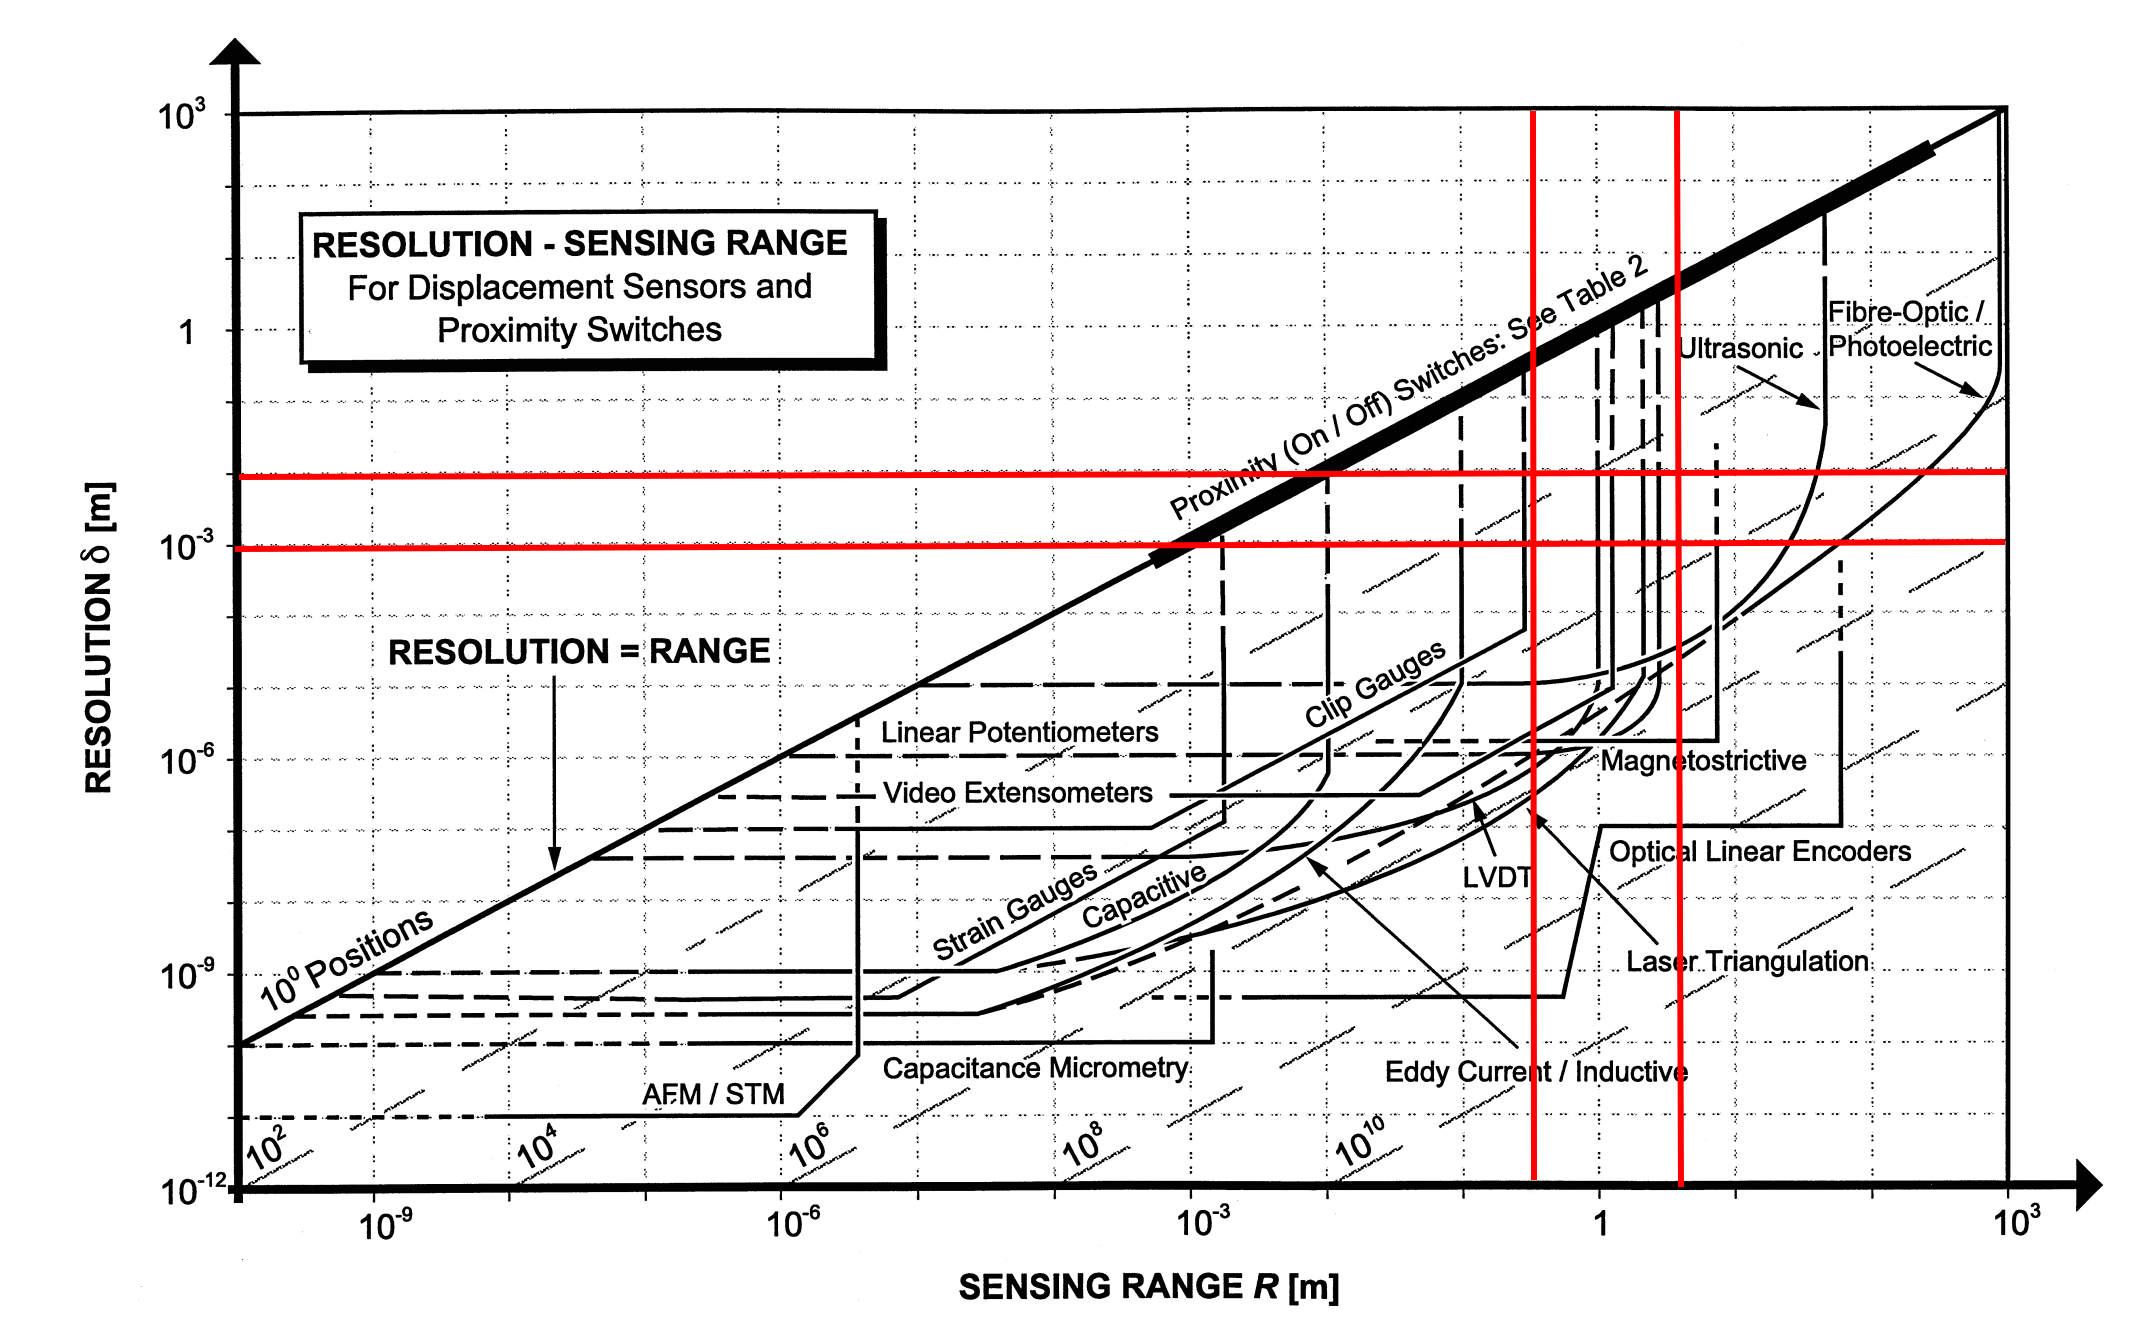
\includegraphics[width=\textwidth]{DistanzSensor}

Daraus schliessen wir das Ultraschall oder Photoelektrische
Sensoren für unsere Anwendung am Besten geeignet sind.

\subsubsection{Distanz Messung in Z-Richtung}
\label{app:ssec:DistMessZ}
Assistieren der Bilderkennung beim erkennen von Hindernissen und
abschätzen der Z-Höhe des Ladegutes. Je nach dem was für einen Motor gewählt
wird kann dieser zur Abschätzung beitragen wie auch der Beschleunigungssensor
in Z-Richtung. Je nach Grösse der Schwankungen in Y-Richtung kann das Gyroskop
in Y-Richtung auch zur präzise Messung beitragen.

\vspace{1em}
\noindent
\begin{tabular}{|p{0.2\textwidth}|p{0.8\textwidth}|}
  \hline
  \textbf{Anforderung} & \textbf{Grösse} \\
  \hline
  Reichweite & 60cm-110cm \\
  \hline
  Genauigkeit & 1cm \\
  \hline
\end{tabular}

\vspace{1em}
\noindent
\begin{tabular}{|p{0.2\textwidth}|p{0.15\textwidth}|p{0.15\textwidth}|p{0.4\textwidth}|}
  \hline
  \textbf{Name} & \textbf{Interface} & \textbf{Preis} & \textbf{Datenblatt} \\
  \hline
  VCNL4200 & $\text{I}^2\text{C}$ & 3 CHF & https://www.vishay.com/optical-sensors/list/product-84430/ \\
  \hline
\end{tabular}

\subsubsection{Distanz Messung in X-Richtung}
\label{app:ssec:DistMessX}
Genaue Positionsbestimmung auf der X-Achse.\\
Mögliche Lösungsansätze (oder Kombination von Lösungsansätze) zu
evaluieren
\begin{itemize}
\item Ultraschall oder Photoelektrische Sensoren, obwohl aufgrund der Zeichnung
  das fehlen einer schönen Fläche vorne oder hinten zum Problem werden könnte.
\item Positionsbestimmung durch messen abgefahrener Strecke
\item Positionsbestimmung durch messen der Beschleunigung in X-Richtung
\item Positionsbestimmung durch Feature-Tracking
\end{itemize}

\section{Positionsanzeige}
\label{app:sec:PosAnz}
\vspace{1em}
\noindent
\begin{tabular}{|p{0.3\textwidth}|p{0.02\textwidth}|p{0.02\textwidth}|p{0.02\textwidth}|p{0.5\textwidth}|}
	\hline
	\textbf{Beschreibung} & \textbf{U} & \textbf{N} & \textbf{B} & \textbf{Quelle} \\
	\hline
	LCD Modul & 1 & 3 & 4 & https://www.sparkfun.com/products/9394 \\
	\hline
	RPI Bluetooth & 2 & 3 & 5 & https://github.com/EnableTech/raspberry-bluetooth-demo \\
	\hline
\end{tabular}

\section{Energieversorgung}
\label{app:sec:EngVers}
\vspace{1em}
\noindent
\begin{tabular}{|p{0.3\textwidth}|p{0.02\textwidth}|p{0.02\textwidth}|p{0.02\textwidth}|p{0.5\textwidth}|}
	\hline
	\textbf{Beschreibung} & \textbf{U} & \textbf{N} & \textbf{B} & \textbf{Quelle} \\
	\hline
	LiPo & 1 & 3 & 4 & https://hobbyking.com/en\_us/lipo.html \\
	\hline
	Ladegerät & 1 & 3 & 4 & https://hobbyking.com/en\_us/imax-b6ac-v2-professional-balance-charger-discharger.html \\
	\hline
	Batterie-Packet & 1 & 1 & 2 & https://www.conrad.ch/de/batteriehalter-4x-mignon-
	aa-kabel-l-x-b-x-h-63-x-55-x-16-mm-mpd-ba4aaw-1555
	538.html?sc.ref=Search\%20Results
	\\
	\hline
\end{tabular}

\section{Last anheben/senken}
\label{app:sec:LastAnhub}
\begin{tabular}{|p{0.3\textwidth}|p{0.02\textwidth}|p{0.02\textwidth}|p{0.02\textwidth}|p{0.5\textwidth}|}
	\hline
	\textbf{Beschreibung} & \textbf{U} & \textbf{N} & \textbf{B} & \textbf{Quelle} \\
	\hline
	Antriebsmotor, 12VDC, 3W, 0.05Nm & 3 & 1 & 4 &
	http://ch.farnell.com/airpax/9904-120-52602/getriebemotor-12v-dc-330-u-min/dp/147874  \\
	\hline
	div. Typen & 1 & 2 & 3 & http://www.directindustry.de/prod/johnson-electric/product-665-470175.html\\
	\hline
	12VDC, \textbf{85rpm}, 2~3W & 1 & 3 & 4 & https://goo.gl/NfN4xx\\
	\hline
	Gleitlager, 3mm & 1 & 2 & 3 & http://www.cncshop.at/index.php?k=165\\
	\hline
\end{tabular}

\section{Startsignal}
\label{app:sec:Startsignal}
\subsection{Mechanisch – Knopf}
\label{app:ssec:StartKnopf}
Keine Datenübertragung, Einfach, keine Parameter

\subsection{Bluetooth}
\label{app:ssec:BT}
Datenübertragung, direkt Sicht nötig, Parameter möglich, Geringer Energiebedarf, aufwendiges Pairing.
Kann gleichzeitig verwendet werden um während des Entwicklungs- und Test-Prozesses Daten (v.a. Software-Updates) an die Laufkatze zu senden. Zudem könnten während Entwicklung und Betrieb Daten an eine Auswertungseinheit (Debugging) (z.B. Laptop oder anderes Mobilgerät) gesendet werden.

\subsection{WiFi}
\label{app:ssec:WLAN}
Datenübertragung, weite Distanzen möglich, Userinterface einfach zu bauen, Parameterübergabe möglich, Verbinden dauert unter Umständen lange, Ad-hoc Verbindungen
Kann gleichzeitig verwendet werden um während des Entwicklungs- und Test-Prozesses Daten (v.a. Software-Updates) an die Laufkatze zu senden. Zudem könnten während Entwicklung und Betrieb Daten an eine Auswertungseinheit (Debugging) (z.B. Laptop oder anderes Mobilgerät) gesendet werden.

\subsection{Akustisch}
\label{app:ssec:Sonic}
Mikro nötig, Falscherkennung Signal als Risiko, zusätzliche Bibliotheken welche sonst nicht benötigt werden.

\subsection{Licht}
\label{app:ssec:FiatLux}
Einfach, Problem Abschirmung \& Fremdsignale.

\vspace{1em}
\noindent
\begin{tabular}{|p{0.3\textwidth}|p{0.02\textwidth}|p{0.02\textwidth}|p{0.02\textwidth}|p{0.5\textwidth}|}
	\hline
	\textbf{Beschreibung} & \textbf{U} & \textbf{N} & \textbf{B} & \textbf{Quelle} \\
	\hline
	Lichtsensor bauen & 2 & 1 & 3 & http://www.instructables.com/id/Highly-sensitive-Arduino-light-sensor/ \\
	\hline
\end{tabular}


\section{Endschalter}
\label{app:ssec:FinButton}
\begin{tabular}{|p{0.3\textwidth}|p{0.02\textwidth}|p{0.02\textwidth}|p{0.02\textwidth}|p{0.5\textwidth}|}
	\hline
	\textbf{Beschreibung} & \textbf{U} & \textbf{N} & \textbf{B} & \textbf{Quelle} \\
	\hline
	Endschalter Hebelarm & 1 & 2 & 3 & https://goo.gl/W2no2b\\
	\hline
	Hebelarm & 1 & 2 & 3 & http://www.robotshop.com/ca/en/micro-contact-limit-switch.html\\
	\hline
\end{tabular}

\section{Last greifen}
\label{app:ssec:GrabbyGrabbyThingy}
\begin{tabular}{|p{0.3\textwidth}|p{0.02\textwidth}|p{0.02\textwidth}|p{0.02\textwidth}|p{0.5\textwidth}|}
	\hline
	\textbf{Beschreibung} & \textbf{U} & \textbf{N} & \textbf{B} & \textbf{Quelle} \\
	\hline
	Greifer, Krangreifer &4 &2 &6 & https://goo.gl/TCDBLD \\
	\hline
	Greifer, Greifer Festo &3 &1 &4 & https://goo.gl/4LkLtu\\
	\hline
	Greifer Festo 2 &4 &3 &7 & https://goo.gl/ZBjYKg\\
	\hline
	Zylinder Elektronisch, Phoenix Mecano &3 &3 &6 & https://goo.gl/zbZbAp\\
	\hline
	Elektromagnet maqna &3 &4 &7 & https://goo.gl/RpFgQZ\\
	\hline
	Goudsmit Elektro-magneten &3 &2 &5 & https://goo.gl/FHBsJE\\
	\hline
	Elektromagnet Auslegung &4 &4 &8 & https://goo.gl/H2XLqz\\
	\hline
	Elektro-permanent-magnet - Analytische und Experimentelle Methodologie und Konstruktion & 5 & 3 & 8 & https://goo.gl/29kkM8\\
  \hline
\end{tabular}

\chapter{Grobkonzept / Evaluation Prinzipien}
\label{app:ch:Grobkonzept}
\section{Morphologischer Kasten}
\label{app:sec:MorphKasten}
Auf der folgenden Seite sehen Sie den morphologischen Kasten mit den Pfaden zu den Konzepten. Danach werden die einzelnen Komponenten im Detail betrachtet.


\includepdf[pages=2]{Morphkasten.pdf}

\section{Mechanik}
\label{app:sec:Mech}
\subsection{Evaluation Antrieb Variante 1: Reibung mit Brückenaufhängung}
\label{app:ssec:EvalAntrieb1}
Der Antrieb mittels Reibung erfolgt durch einen Motor, welcher Drehmoment auf ein Antriebsrad überträgt. Dieses wandelt über Reibung rotatorische Bewegung in translatorische um. So wird eine Vorwärtsbewegung erzeugt. Die Materialpaarung des Antriebsrades zum Seil, welches in unserem Fall ein Stahllitzenseil ist, entscheidet dabei massgeblich die resultierende Haftung. Dabei muss auch beachtet werden, dass durch die Aufhängung auf zwei Rädern die Gewichtsaufnahme pro Rad halbiert wird und somit die Reibungskraft des Antriebsrades verkleinert wird.

Die Aufhängung wird durch eine Art von Brückenaufhängung erreicht. Dabei laufen zwei Räder oberhalb des Seils, wobei eines der Beiden das Antriebsrad ist. Der Vorteil der Brückenaufhängung, bei der die beiden Tragräder relativ weit voneinander entfernt sind, ist dass die Aufhängung stabil gegen pendeln um die y-Achse ist. Das heisst, das Pendeln wird durch die breite Abstützung der Räder bestmöglich reduziert. Die breite Abstützung ermöglicht, dass ein grosses Drehmoment aufgenommen werden kann. Weiter muss berücksichtigt werden, dass der Durchhang durch die breite Abstützung der Räder etwas reduziert werden kann. Dieser kann mittels Trigonometrie einfach errechnet werden. Ein Nachteil, im Vergleich zur Variante 2: Reibung mit Gegendruckrad ist, dass für die Lastanhebung ein weiteres Gelenk entwickelt werden muss.

\subsection{Evaluation Antrieb Variante 2: Reibung mit Gegendruckrad}
\label{app:ssec:EvalAntrieb2}
Bei dieser Variante gibt es, neben einem Gegendruckrad, nur ein tragendes Rad. Das antreibende Rad könnte entweder das Tragrad oder auch das Gegendruckrad sein. Ein Vorteil dieser Variante ist, dass ein höherer Druck des Rades auf das Tragseil erreicht werden kann. Damit kann eine höhere Reibungskraft erzielt werden. Ein weiterer Vorteil dieser Konstruktion ist, dass kein weiteres Gelenk für den Steigungswinkelausgleich entwickelt werden muss. Die ganze Konstruktion hängt somit immer senkrecht zum Boden.

Der Nachteil dieser Konstruktion ist, dass eine Stabilität gegen Pendeln um die y-Achse schwer zu erreichen ist. Da der Drehpunkt auf nur einem Rad ist, kann kein Drehmoment aufgenommen werden.

\subsection{Evaluation Antrieb Variante 3: Reibung mit Doppelaufhängung}
\label{app:ssec:EvalAntrieb3}
Dieses Prinzip ist eine aus den Varianten Reibung mit Brückenaufhängung und Reibung mit Gegendruckrad. Einerseits werden hier wie bei der Brückenaufhängung zwei tragende Räder eingesetzt, womit ein wenig Drehmoment aufgenommen werden kann. Doch es kann auch ein wenig Steigungswinkelausgleich erzielt werden. Eventuell müsste hier aber noch eine zusätzliche Pendeldämpfung um die y-Achse entwickelt werden.


\subsection{Evaluation Lastaufnahme per Seilwinde}
\label{app:ssec:EvalLast}
Die Seilwinde ist eine Vorrichtung, welche Hauptsächlich aus einer Seiltrommel, Seil und Antrieb besteht. Die Lastaufnahme geschieht durch Zugkräfte am Seil, welche durch das Drehmoment vom Motor erzeugt wird.

\subsubsection{Antrieb der Seiltrommel}
\label{app:ssub:Seilantrieb}
Der Antrieb einer Seiltrommel kann mittels eines Servo- oder Schrittmotors realisiert werden. Überschlägige Berechnungen ergeben ein Mindestdrehmoment von $\simeq$ 30Nmm und eine Mindestleistung von $\simeq$ 180mW. Diese Leistung genügt, um eine Masse von 100g mit einer Geschwindigkeit von 10cm/s zu heben, was für unsere Anwendung ausreicht.
\newline \newline
$g=9.81m/s^{2}$;\hspace{5mm} $r=0.03m$;\hspace{5mm} $m=0.15kg$;\hspace{5mm} $v=0.1m/s$;\hspace{5mm} $\eta=0.8$ \newline \newline
$P=\frac{M*\omega}{\eta}=\frac{m*g*r*v}{r*\eta}=\frac{m*g*v}{\eta}=\frac{0.15*9.81*0.1}{0.8}=0.18W$

\subsubsection{Seil}
\label{app:ssec:Seil}
Für das Seil kann ein Nähfaden, Fischerschnur oder ein dünnes Litzenseil verwendet werden. Der Nähfaden ist flexibler als die Fischerschnur, hat aber eine geringere Zugfestigkeit. Das Litzenseil kann vorläufig ausgeschlossen werden, da die Steifigkeit sehr gross ist und keine massiven Zugkräfte erwartet werden. Zudem könnte mit der Fischerschnur und dem Nähfaden einen Seilzug realisiert werden, um die Leistung des Motors zu verringern. Dies aber auf kosten der Hubgeschwindigkeit.

\subsubsection{Seiltrommel}
\label{app:ssec:Seiltrommel}
Die Seiltrommel kann aus Aluminium, Stahl oder Kunststoff gefertigt werden. Alu und Kunststoffe haben die kleinere Dichte als Stahl und sind somit besser geeignet. Die Kunststofftrommel kann auch im 3D-Drucker hergestellt werden. Neben der Gewichtseinsparung allgemein ist auch das Trägheitsmoment kleiner, was den Motor entlastet.

\subsubsection{Fazit}
\label{app:ssec:Fazit}
Der einfache Aufbau einer Seiltrommel ermöglicht eine flexible und kompakte Bauweise verbunden mit einer kostengünstigen Fertigung. Die Schwierigkeit besteht darin, die Last möglichst schwingungsfrei zu transportieren. Zu beachten ist, dass durch das Aufwickeln des Seils der Durchmesser der Seiltrommel zunimmt, was sich dann auf die Hubgeschwindigkeit und das Moment auswirkt.

\subsection{Evaluation Lastaufnahme per Zahnstange}
\label{app:ssec:EvalLastZahn}
Durch die grössere Steifigkeit einer Zahnstange gegenüber einem Seil sind keine Pendelbewegungen innerhalb der Kontur möglich. Dadurch wird das schwingungsfreie Anheben und Absetzen der Last deutlich einfacher. Die Schwierigkeit besteht darin, eine Distanz von Mindestens 600mm in Z-Richtung zu überwinden. Bedingt durch die Tatsache, dass die Last und das Tragseil sich in der gleichen Z-Ebene befindet, muss die Zahnstange leicht in Y-Richtung versetzt werden. \newline
Überschlägige Berechnungen für den Antrieb ergeben die gleichen Ergebnisse wie beim Antrieb der Seilwinde (siehe \ref{app:ssub:Seilantrieb}). Bei der Zahnstange ist aus Gewichts- und Kostengründen eine Ausführung aus Kunststoff sinnvoll. Passende Zahnritzel sind online in der Ausführung Edelstahl oder Kunststoff verfügbar, wobei für die vorgesehene Anwendung die Kunststoffausführung vollkommen ausreicht. Eine präzise Führung kann durch mehrere Rollen rund um die Zahnstange gewährleistet werden. Alternativ ist auch ein passendes Gegenstück mit guten Gleiteigenschaften, welches gegenüber vom Antrieb montiert wird, möglich. Dabei ist zu beachten, dass Reibung an den Führungsschiene eine lokale Erwärmung des Kunststoffes zur Folge hat. Diese Ausdehnung kann somit zu Abweichungen zur Senkrechten führen.

\subsection{Evaluation Aufhängung ungedämpft}
\label{app:ssec:EvalAufhangUngedaempft}
Diese Möglichkeit ist die einfachste Variante für die Aufhängung. Es werden keine Dämpfer oder sonstige Komponenten für den Ausgleich eingesetzt. Deshalb ist diese Variante leicht, günstig und mit einem geringen Arbeitsaufwand realisierbar. Jedoch wird durch Beschleunigung das ganze Gerät in Schwingung geraten, da diese Aufhängungsvariante nicht in der Lage ist, diese zu Dämpfen. Solche Schwingungen haben einen negativen Einfluss auf die Absetzgenauigkeit und auf den Antrieb am Seil, da zusätzliche Kräfte wirken.

\subsection{Evaluation Aufhängung unten, gelenkig und gedämpft}
\label{app:ssec:EvalAufhangUnten}
Durch die unten gelenkige und gedämpft gelagerte Aufhängung kann die Winkeländerung, welche durch den Seildurchhang verursacht wird, kompensiert werden. Dabei hängt die Last durch den Schwerpunkt immer senkrecht nach unten. Durch das Gelenk (ähnlich wie bei einer Gondelbahn) wird der ganze Aufbau aber empfindlich gegen pendeln, da das Gelenk kein Drehmoment aufnehmen kann. Dieses wird beispielsweise durch die Beschleunigung bei Anfahren oder Abbremsen erzeugt. Zudem kann sich, je nach Aufbau, der Schwerpunkt der Laufkatze beim Anheben und Absetzen der Last ändern, was wiederum ein Drehmoment erzeugt. Mit Dämpfern kann das Drehmoment aufgenommen und ein Pendeln minimiert werden. Diese Dämpfer werden dann, im Prinzip einer Pendelstütze in der Mechanik, am einen Ende am Fahrwagen und am anderen Ende am unteren Aufbau montiert. Zudem soll der Dämpfer möglichst schräg angestellt sein, damit er die Pendelbewegung aufnehmen kann.

\subsection{Evaluation Last per Haken greifen}
\label{app:ssec:EvalLastHaken}
Ein Haken um die Last anzuheben überzeugt mit seiner einfachen Konstruktion und einer Sicherung gegen das Verlieren der Last. Dafür ist aber sicherlich das An- und Abhängen der Last an den definierten Punkten schwierig, da der Haken zuerst gesenkt und danach ausgefahren werden muss. Auch bei der Aufnahme der Last muss die Öffnung des Hakens der Last getroffen werden. Falls dies fehlschlagen würde, hätte dies ein grosser Punktabzug die Folge. Für diese Variante ist die Abstimmung und Kommunikation der beteiligten Komponenten sehr wichtig.

\subsection{Evaluation Last per Dauermagnet greifen}
\label{app:ssec:EvalLastMagnet}
Mit einem Dauermagnet ist das Greifen der Last sehr einfach, da der Dauermagnet auch bei einer ungenauen Annäherung an die Last dessen Haken anziehen. Auch der Transport über die Hindernisse ist praktisch risikofrei vom Verlust der Last. Die Probleme liegen ausschliesslich beim Absetzen der Last, da der Dauermagnet nur durch starke Gewalteinwirkung, grosse Hitze oder ein um einiges stärkeres Magnetfeld entmagnetisiert werden kann. Diese Möglichkeiten bestehen technisch, in diesem Projekt jedoch aus Kosten-, Grössen-, und Gewichtsgründen nicht. Eine Konstruktion, welche den Magneten mechanisch von der Last trennt, wäre deshalb nötig um die Last absetzen zu können.

\subsection{Evaluation Last per Elektromagnet greifen}
\label{app:ssec:EvalLastElektroMagnet}
Um die Last mit einem Elektromagnet zu greifen ist eine präzise Positionierung in x-y notwendig, da das Magnetfeld quadratisch abnimmt, und eine Anziehung des Magnets an die Last dadurch nicht gut funktioniert. Es wurde versucht die Grundfläche des Elektromagnets zu vergrössern, wobei sich herausstellte das die gewählte Geometrie ungeeignet war. Weitere Schwierigkeiten sind bei der Wahl des Durchmessers des Kupferdrahtes entstanden. Um einen genügend grossen Strom zu erreichen ist ein kleiner Widerstand notwendig. Dies hatte zur Folge, dass der Elektromagnet bei kleinen Spannungen betrieben werden musste, damit dieser nicht zu überhitzen. Eine Pulse Width Modulation ist notwendig um den Elektromagnet mit höheren Spannungen zu betreiben. Der Elektromagnet ist schwieriger zu realisieren als einen Haken, kann aber die Last schneller greifen.

\subsection{Evaluation Positionsbestimmung per Schrittmotor}
\label{app:ssec:EvalPosBestSchritt}
Eine Positionsbestimmung per Schrittmotor hat den Nachteil, dass bei variabler Last Schritte übersprungen werden können, was die Positionsbestimmung ungenau oder komplett nutzlos machen könnte. Beim Antrieb ist die Last konstant, und darum ist ein Schrittmotor gut geeignet. Für die Positionsbestimmung der Last könnte es schwieriger werden, aber ein Lastdelta von 100g sollte zu Bewältigen sein. Für die Positionsbestimmung der Last ist eine zusätzliche Messung notwendig, da es nur die relative Distanz zum Gefährt messen kann und nicht die absolute Höhe der Lasts.

\subsection{Evaluation Positionsbestimmung per Durchhang}
\label{app:ssec:EvalPosBestDurch}
Durch vorgängiges Evaluieren des Durchhangs, in Abhängigkeit der Position in x-Richtung, mit dem Gewicht der Laufkatze kann eine Funktionsgleichung erstellt werden. Diese kann in Software hinterlegt werden, und damit die Position der Last in z-Richtung, in Abhängigkeit der Position in x-Richtung, berechnet werden. Der Vorteil dieser Variante ist, dass nur ein Sensor für die Positionsbestimmung benötigt wird. Die Funktionsgleichung kann einerseits durch Errechnen ermittelt werden. Anderseits kann durch Anhängen einer Probelast an das Drahtseil, die Kurve durch Auswertung des Versuches ermittelt werden. Der Vorteil der Funktionsgleichung des Versuchs gegenüber der errechneten Funktionsgleichung ist, dass alle Einflussfaktoren wie Rollreibung, Seil Eigengewicht, Ungenauigkeiten etc. berücksichtigt werden. Dies ist durch Berechnen kaum möglich.

\section{Elektronik}
\label{app:sec:ET}
\subsection{Blockdiagramm}
\label{app:ssec:BlockDiag}

\begin{figure}[h!]
  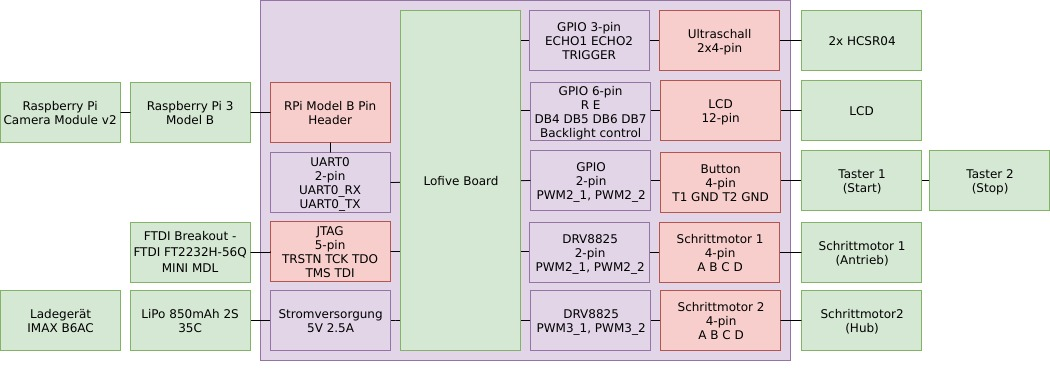
\includegraphics[keepaspectratio,width=\textwidth]{BlockdiagrammElektronik}
  \caption{Blockdiagramm}
  \label{fig:ElektronikBlockdiagramm}
\end{figure}

\newpage
\subsection{Evaluation Time of Flight Sensor}
\label{app:ssec:EvalTOF}
Als TOF-Sensor wird jede Art von Sensor bezeichnet, welche die Zeit misst, die ein Objekt (z.B. Lichtstrahl oder Schallwelle) benötigt um von der Quelle zum Messpunkt und zurück zum Sensor zu gelangen. So kann die Distanz sehr genau bestimmt werden. Jedoch zeigt ein Blick in den Katalog von Mouser und Distrelec, dass Sensoren welche bis 3.5m taugen, mehr als 500.- Fr kosten.

\subsection{Evaluation Positionsbestimmung mit Beschleunigungssensor}
\label{app:ssec:EvalPosBestBeschleunigung}
Mit einem Beschleunigungssensor kann die Beschleunigung sehr exakt bestimmt werden. Daher wird davon ausgegangen, dass durch zweifaches Integrieren der Messdaten ein Bewegungsverlauf in X und Z-Achse realisiert werden kann. Der Vorteil an dieser Lösung ist, dass der Roboter unabhängig vom Versuchsaufbau seine Positionsänderung bestimmt. Je nach Genauigkeit können der Antrieb und der Aufzug somit auch mit DC-Motoren realisiert werden. Jedoch kann erst nach der Umsetzung dieser Variante mit Sicherheit gesagt werden, dass diese Ausführung der Positionsbestimmung genau genug ist.

\subsection{Evaluation Lofive Board}
\label{app:ssec:EvalLofive}
Das Lofive Board enthält einen RV32IMAC Prozessor. Der RV32IMAC Prozessor ist
ideal für unsere Anwendung. Es ist der erste in Silikon verfügbare RISCV
Microcontroller (hat keine MMU). RISCV ist eine neue RISC Komputerarchitektur
die sich durch Patentfreiheit, Erweiterbarkeit, Einfachheit und Performance von
anderen Komputerarchitekturen unterscheidet. RV32IMAC ist ein freier Prozessor,
insofern das der Quellcode offen ist. Custom silicon auf der Basis von RV32IMAC
wird schon in kleinen Quantitäten (~10000) von Sifive angeboten, und kann so
auf Anwendungen zugeschnitten werden.

Im Gegensatz zur GCC Toolchain ist die LLVM Toolchain noch nicht vollständig
geupstreamt, das heisst das sie vom Quellcode kompiliert werden muss. Für den
Einsatz von Rust ist die LLVM Toolchain eine Voraussetzung. Rust funktioniert
gut auf dem RV32IMAC, ein RTOS wie RTFM muss noch portiert werden (TODO:
Winterferien). Falls unvorhergesehenen Komplikationen auftreten kann C
eingesetzt werden.

\subsection{Evaluation Arduino UNO}
\label{app:ssec:ArduinoUno}
Arduino ist ein Entwicklerboard, welches einfach zu programmieren ist und wozu bereits diverse zusätzliche Komponenten zur Verfügung stehen. Auf dem Bord stehen 6 I/O-Pins sowie 6 Analoge Inputs zur Verfügung. Für die Kommunikation mit dem IT-Bord ist es möglich via serieller Schnittstelle (UART) zu kommunizieren. Eine IDE wird spezifisch für das Arduino-Bord zur Verfügung gestellt. Programmiert wird in C/C++ und wird erweitert durch einige Arduino-Libraries.

\subsection{Energie und Stromversorgung}
\label{app:ssec:EnergieStrom}
Der Stromverbrauch wird in der Tabelle \ref{tab:stromverbrauchstabelle}
aufgelistet.

\noindent
\begin{table}[h!]
	\begin{tabular}{|p{0.6\textwidth}|p{0.3\textwidth}|}
		\hline
		\textbf{Komponente} & \textbf{Stromverbrauch [A]} \\
		\hline
		RaspberryPi & min 1.3A, 2A \\
    \hline
    Lofive Board & typ 8mA, max 150mA \\
    \hline
    Schrittmotor Antrieb & 2 Phasen a max 1.68A \\
    \hline
    Motor Lastanhebung & 150mA? \\
    \hline
    Anzeige & 150mA? \\
		\hline
	\end{tabular}
	\caption{Stromverbrauch des Roboters}
	\label{tab:stromverbrauchstabelle}
\end{table}

\subsection{Elektronik Kosten}
\label{app:ssec:ETKosten}
Um die Kosten der Elektronischen Komponenten zu erfassen, werden in der Tabelle
\ref{tab:elektronikkosten} alle Bauteile aufgelistet, welche für die Umsetzung
in Frage kommen. \parencite{Meier2013} \parencite{ReicheltE2017} \parencite{RenoDenver2017}

\noindent
\begin{table}[h!]
	\begin{tabular}{|p{0.7\textwidth}|p{0.3\textwidth}|}
		\hline
		\textbf{Komponente} & \textbf{Preis [CHF]} \\
		\hline
		LoFive/Arduino & 25 \\
		\hline
		Beschleunigungssensor & 5 \\
		\hline
		Elektromagnet & 11 \\
		\hline
		\underline{\textbf{Total}} & \underline{\textbf{41}} \\
		\hline
	\end{tabular}
	\caption{Kosten (exkl. Versand)}
	\label{tab:elektronikkosten}
\end{table}


\section{Informatik}
\label{app:sec:Inf}

\subsection{Evaluation Plattformen und Programmiersprachen}
\label{app:ssec:EvalPlattPrg}
Das Raspberry Pi ist ein Einplatinencomputer in der Grösse einer Kreditkarte. Das Ein-Chip-System von Broadcom läuft mit einem ARM-Mikroprozessor. Durch seine Bekanntheit, der vielen Module die es dazu fertig gibt, sowie seinem Preis ist das Raspberry Pi Pionier auf dem Bereich der Einplatinencomputer.

\begin{itemize}[noitemsep]
	\item Quad Core 1.2GHz Broadcom BCM2837 64bit CPU
	\item 1GB RAM
	\item BCM43438 WLAN und Bluetooth Low Energy (BLE) auf dem Board
	\item 40-pin erweitertes GPIO
	\item 4 USB2 Ports
	\item 4 Pol Stereo Ausgang und Composit Video Port
	\item Full-Size HDMI
	\item CSI Kamera Port um eine Raspberry Pi Camera anzuschliessen
	\item DSI Bildschirmausgang um einen Raspberry Pi Touchscreen anzuschliessen
	\item MicroSD Anschluss um das OS und Daten zu speichern
	\item Die geschaltete Micro USB Stromzufuhr wurde auf bis zu 2.5A erhöht
\end{itemize}\parencite{RaspberryPiFoundation2017}


Die Konkurrenten des Raspberry Pi sind meistens leistungsstärker, dadurch aber auch teurer. Was beim Raspberry Pi immer wieder betont wird, ist die riesige Community und deren Unterstützung. Man kann mit hoher Wahrscheinlichkeit davon ausgehen, dass Teilprobleme, welche wir in diesem Projekt haben werden, bereits von Anderen teilweise oder ganz gelöst und dokumentiert wurden.

Diese Unterstützung einer grossen Community und unsere eigene Unzulänglichkeiten betrachtend, haben wir uns für das Raspberry Pi entschieden.

\begin{multicols}{2}
	\textbf{Vorteile}
	\begin{itemize}[label={+},noitemsep]
		\item OS Installation möglich
		\item Erweiterbarkeit
		\item Unterstützung diverser Programmiersprachen
		\item Hoher Bekanntheitsgrad
		\item Grosse Community
		\item Niedriger Preis
	\end{itemize}
	\columnbreak
	\textbf{Nachteile}
	\begin{itemize}[label={-},noitemsep]
		\item Ausführung von Befehlen langsamer als bei einfachem Mikrocontroller
	\end{itemize}
\end{multicols}

Python ist eine objektorientiere Programmiersprache, welche den Ruf hat, sehr einfach zu erlernen zu sein. Python wird  zur Laufzeit in Maschinensprache übersetzt. Die Grenzen liegen auf der systemnahen Programmierung (z.B. bei
Gerätetreibern oder optimalen Geschwindigkeiten).

Immer auch unsere eigenen Erfahrungen und Vorkenntnisse im Kopf behaltend, haben wir uns im Informatikerteam entscheiden mit Python zu beginnen.

\begin{multicols}{2}
	\textbf{Vorteile}
	\begin{itemize}[label={+},noitemsep]
		\item Objektorientiert
		\item Einfach zu lernen
		\item Umfangreiche Bibliotheken
	\end{itemize}
	\columnbreak
	\textbf{Nachteile}
	\begin{itemize}[label={-},noitemsep]
		\item Geschwindigkeit im Vergleich zu C
		\item Spezieller Syntax (bspw. keine Semikolons, Indent hat Bedeutung)
	\end{itemize}
\end{multicols}

Die Nachteile von Python liegen vor allem in der Geschwindigkeit der Interpretation, da Python im Vergleich zu C eine interpretierte und keine vorkompilierte Sprache ist. Wir behalten uns vor, den erarbeiteten Code zu C/C++ zu portieren, sollte Geschwindigkeit ein Problem werden.

Bei der Programmiersprache C werden einzelne Anweisungen als Folge zusammengestellt, welche nacheinander ausgeführt werden. C ist sehr maschinennah, weshalb sie auch als sehr schnell gilt. C++ erweitert C mit unter anderem Objektorientiertheit, verbesserte Typensicherheit und Exception Handling. C++ Compiler können den meisten C Code kompilieren. \parencite{Mishra2015}

\begin{multicols}{2}
	\textbf{Vorteile}
	\begin{itemize}[label={+},noitemsep]
		\item Systemnah
		\item Geschwindigkeit
		\item Mächtig
	\end{itemize}
	\columnbreak
	\textbf{Nachteile}
	\begin{itemize}[label={-},noitemsep]
		\item Komplex
		\item Keine voreingebauten Sicherheitsbegrenzungen
	\end{itemize}
\end{multicols}

\subsection{Evaluation Kommunikation zwischen Elektronikkomponenten}
\label{app:ssec:EvalKomm}
Zwischen dem RaspberryPi und dem Elektronikerboard soll der Informationsaustausch über eine serielle Schnittstelle erfolgen. Entweder über USB oder über die dedizierten Pins asynchron (UART).

\subsubsection{UART}
\label{app:ssec:EvalUART}
Für die Verwendung einer Kommunikation mit einer asynchronen, seriellen UART-Schnittstelle können jeweilige PINs verwendet werden.

Auf dem RaspberryPi können Pin 8 (Tx) und Pin 10 (Rx) verwendet werden.

Die Pins können für Testzwecke direkt via Kabel miteinander verbunden werden. Im Endausbau soll diese Verbindung jedoch über einen eigenes angefertigten Print laufen. So wird auch sichergestellt, dass beide Boards einen gemeinsamen GROUND haben.

UART muss auf dem RaspberryPi manuell aktiviert werden.  Zusätzlich muss das integrierte Bluetooth-Modul deaktiviert werden, sodass die genannten Ports nicht "miniUART"\ verwenden.

Für die serielle Übertragung müssen Baudrate, Port, Databits, Parity Check, Stopbits und flow control sowie ein genaues Nachrichtenformat definiert werden.

\subsubsection{USB}
\label{app:ssec:EvalUSB}
Für die Verwendung einer seriellen Schnittstelle über USB könnte ein 5V Serial TTL Kabel verwendet werden. Dafür müssten die jeweiligen Treiber installiert sein, in Raspberry Pi würde dieses dann unter \colorbox{lightgrey}{/dev/ttyUSB} zu finden sein.

Ansteuern kann man dann diesen Port über die Python Bibliothek pySerial. \parencite{Liechti2017} Auch hier müssten Baudrate, Bytesize, Parität und Kontrollbits selber definiert werden. Das Nachrichtenformat für den Austausch zwischen RasPi und Elektrikerboard müsste ebenfalls entwickelt werden.

\subsection{Evaluation Zielerkennung per Bilderkennung}
\label{app:ssec:EvalZielErkBild}
Zur Bilderfassung wird eine RaspberryPi Camera v2 verwendet. Das Camera Modul v2 besitzt die Dimensionen 25 x 24 x 9 mm, wiegt ca. 3g und kostet ca. 44 CHF.
Sie hat einen Sony IMX219 8-Megapixel Sensor. Die Kamera wird über das CSI-Schnittstelle angeschlossen und gesteuert. Sie ist für Anfänger geeignet, biete jedoch trotzdem viele Funktionen für Fortgeschrittene Nutzer.
Bereits während der Technologierecherche tauchten viele nützliche Anleitungen auf, in welchen das Camera Module v2 genutzt wurde.
Zur Ansteuerung mit Hilfe der Programmiersprache Python gibt es eine entsprechende Python-Bibliothek: picamera.

\begin{multicols}{2}
	\textbf{Vorteile}
	\begin{itemize}[label={+},noitemsep]
		\item Einfach zu verbauen
		\item Einfach anzusteuern
		\item Libraries für verschiedene Programmiersprachen
		\item kleine Bauform
		\item grosse Community und viele Projekte
	\end{itemize}
	\columnbreak
	\textbf{Nachteile}
	\begin{itemize}[label={-},noitemsep]
		\item $\frac{1}{10}$ des Budgets
	\end{itemize}
\end{multicols}

\noindent
Die Verwendung einer kostengünstigeren USB-Kamera wird ausgeschlossen.

\begin{multicols}{2}
	\textbf{Vorteile}
	\begin{itemize}[label={+},noitemsep]
		\item Unter Umständen günstiger
		\\
		\\
		\\
		\\
		\\
		\\
	\end{itemize}
	\columnbreak
	\textbf{Nachteile}
	\begin{itemize}[label={-},noitemsep]
		\item Grosse Bauform
		\item Spezielle Treiber nötig (unter Umständen müssen diese selber entwickelt werden)
		\item meist schwerer
		\item kleine Community für solche Projekte
	\end{itemize}
\end{multicols}

\subsubsection{Bilderkennungsbibliotheken}
\label{app:ssec:BilderkBib}
Die beiden grossen, aktiv entwickelten Bibliotheken für computerisierte Bildverarbeitung sind OpenCV (Open Computer Vision) und imageJ (und dessen Derivate).

OpenCV ist hauptsächlich in C++ entwickelt, besitzt aber Schnittstellen zu C, Python, Java und Octave/Matlab. Für viele sonstige Sprachen wurden Wrappers entwickelt. OpenCV wird offen entwickelt, ist frei nutzbar und auf Bilderkennung ausgelegt.

Im Gegensatz dazu ist ImageJ hauptsächlich für Java entwickelt worden, und dient der Bildbearbeitung im wissenschaftlichen Umfeld. Das Problem liegt darin, dass ImageJ weniger auf Mustererkennung (Gesichter, Formen Perspektivisch) und Geschwindigkeit, sondern mehr auf Bildklassifizierung ausgelegt ist. Für unsere Zwecke fällt ImageJ daher weg.

\subsection{Evaluation Zielerkennung per Infrarotsensor}
\label{app:ssec:EvalZielErkInfrarot}
Nebst der klassischen Bilderkennung, wurde auch eine Variante für die Zielerkennung gesucht, welche ohne Kamera funktionieren könnte.

Unserer Ansatz ist es dies mit Hilfe von Infrarot umzusetzen. Hierzu braucht man einen entsprechenden Infrarotsensor (IR-Sensor) und Empfänger.

Um die konzentrischen Bereiche des Zielbereiches zu erkennen, genügt es im Grundprinzip hell und dunkel unterscheiden zu können.

\begin{figure}[h!]
	\centering
	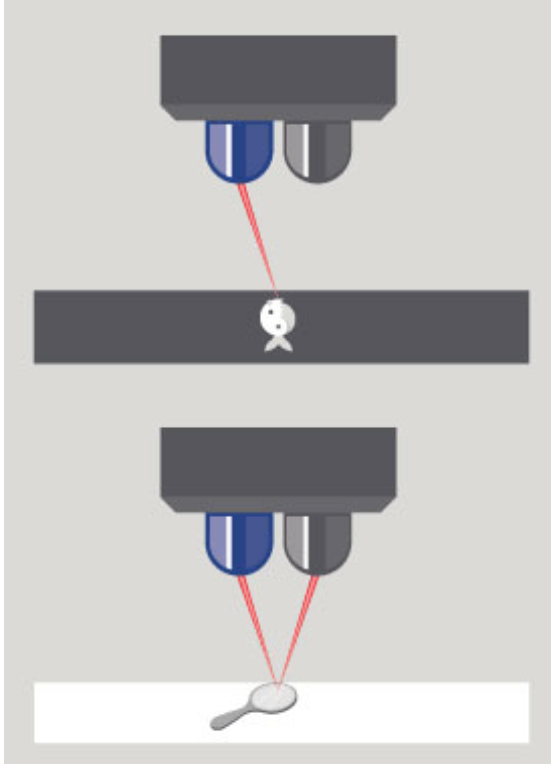
\includegraphics[keepaspectratio,height=5cm]{InfrarotHellDunkel}
	\caption{Wie man mit Infrarot Hell und Dunkel unterscheidet \parencite{Caro2015}}
	\label{fig:InfrarotHellDunkel}
\end{figure}

Der Infrarotsensor, den wir verwenden wollen, ist digital und gibt 1 zurück, wenn Weiß erkannt wird, und 0, wenn Schwarz erkannt wird.

Das Positionieren und Umschliessen von IR-Sender und Empfänger ist sehr wichtig. Sowohl der Sender als auch der Empfänger müssen in einem bestimmten Winkel platziert werden, damit die Erkennung eines Objekts richtig ist - und zwar im Winkel von 45\si{\degree} wie in folgender Abbildung:


\begin{figure}[h!]
	\centering
	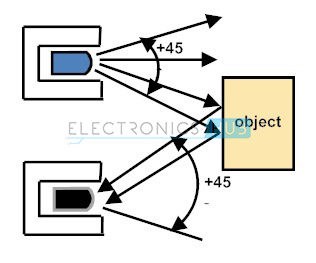
\includegraphics[keepaspectratio,height=5cm]{IRdirectivity.jpg}
	\caption{Platzierung und Umschliessung IR-Sensor \parencite{ElectronicsHub}}
	\label{fig:InfrarotPlatzierung}
\end{figure}


Um Reflexionen von anderen umgebenden Objekten zu vermeiden, müssen sowohl der IR-Sender als auch der IR-Empfänger Umschlossen werden. Das kann mit einem Gehäuse aus Kunststoff, welches mit schwarzer Farbe lackiert ist, umgesetzt werden.

Die durch den Infrarot-Sensor erhaltenen Informationen könnte man nun Aufsummieren um zu erkennen, ob es der abwechslungsweise schwarz/weisse konzentrische Zielbereich ist oder nicht.

Leider muss man für diese Erkennung sehr Nahe am Objekt dran sein. Es handelt sich dabei um einige wenige Zentimeter \parencite{Aswinth2017}. Da sich unsere Laufkatze bis zu 1.2 Meter von der Zielplatte entfernt befinden kann, müsste unsere Infrarot-Konstruktion Nahe am Boden entlang platziert werden können. Um so etwas realisieren zu können, wäre der Einsatz vieler weiterer Sensoren und mechanischen Elementen zwingend.

\begin{multicols}{2}
	\textbf{Vorteile}
	\begin{itemize}[label={+},noitemsep]
		\item Keine Bilderkennung nötig
		\item kleine Bauform
	\end{itemize}
	\columnbreak
	\textbf{Nachteile}
	\begin{itemize}[label={-},noitemsep]
		\item Aufwändige Herstellung
		\item Distanz/Nähe zur Zielplatte
		\item Viele weitere Komponenten nötig damit es funktioniert
	\end{itemize}
\end{multicols}

\chapter{Alternative Lösungskonzepte}
\label{app:ch:AltLoesung}
\section{Lösungsvariante 2}
\label{app:sec:Lvar2}
\subsection{Schnittstellen und Abhängigkeiten}
Bei der Lösungsvariante 2 werden als Mikrocomputer ein RasPi und ein Arduino-Board verwendet. Diese kommunizieren über eine UART-Steckverbindung. Das Protokoll muss wie in der Lösungsvariante 1 abgestimmt sein, um die korrekte Übermittlung der Daten zu gewährleisten. Da das Arduino über eine UART und eine USB Schnittstelle verfügt, wurde die UART Steckverbindung vor allem aus Platzgründen der USB Verbindung vorgezogen.\\
Der Schrittmotor für den Antrieb ist alleine zur Bestimmung der Koordinaten verantwortlich. Mithilfe einer Tabelle, welche den Durchhang an den verschiedenen x-Positionen bestimmt, können die x- und z-Werte ausgelesen werden. Diese Werte sind für die Last Auf- und Abnahme und die Positionsanzeige erforderlich. Diese Werte werden per Bluetooth auf einen Laptop übermittelt und Angezeigt. Die Zielerkennung ist mit einem Infrarotsensor gelöst. Dieser kann Schwarz und Weiss unterscheiden, jedoch nur auf einer Distanz von etwa 20cm. Dies hat zur Folge, dass der Sensor ebenfalls in der Höhe verschiebbar sein muss.\\
Der Antrieb ist mit zwei Rädern auf dem Seil realisiert. Es ist essentiell, dass die Reibkraft zwischen dem Seil und der Räder gross ist, da sonst die Räder rutschen würden bei grosser Steigung. Die Räder sind nicht nahe beieinander, damit keine Schwankungen in x-Richtung entstehen. Die Aufhängung ist ungedämpft vorgesehen, weil keine Schwingungen der Laufkatze gedämpft werden müssen.
Die Last wird mit einem Elektromagnet gegriffen. Der Vorteil daran ist, dass der Elektromagnet nicht exakt an der Position des Hakens sein muss um ihn anzuziehen. Daraus folgt aber auch, dass die Zielplattform nicht exakt getroffen werden kann. Der Elektromagnet wird an einem Seil, welches mit einer Seiltrommel und Elektromotor bewegt wird, befestigt. Das Seil überzeugt mit seiner Einfachheit in der Konstruktion und der kostengünstigen Ausführung. Ein Nachteil ist, dass durch das Seil starke Schwingungen entstehen können, wenn das Gerät beschleunigt wird. Diese wirken sich zusätzlich stark auf die Genauigkeit des Absetzten aus.

\section{Lösungsvariante 3}
\label{app:sec:Lvar3}
Für die dritte Lösungsvariante werden ein LoFive und ein RasPi verwendet. Die Kommunikation erfolgt über eine USB-Schnittstelle.
Das Protokoll muss wie in der Lösungsvariante 1 abgestimmt sein, um die korrekte Übermittlung der Daten zu gewährleisten.\\
Die Datenübertragung erfolgt über eine USB-Schnittstelle. Diese benötigt mehr Platz als eine UART-Schnittstelle, jedoch hat dies der Vorteil dass ein USB nicht verkeht eingesteckt werden kann.
X- und Y-Koordinaten werden mithilfe eines Time of flight sensors bestimmt. Die Werte werden auf einem O/LED-Display angezeigt.
Die Zielerkennung wird mithilfe einer Kamera und einer Bilderkennungssoftware (OpenCV) realisiert.\\
Der Antrieb ist mit 2 Rädern auf dem Seil realisiert. Dies bedingt, dass der Reibwert zwischen Seil und Antriebsrolle genügend gross ist um ein Durchrutschen zu verhindern.\\
Die Last wird mithilfe von einem Dauermagneten gegriffen, welcher mithilfe eines Auslösemechanismus vom Haken der Last getrennt wird. Der Vorteil dieser Variante ist, dass der Haken nicht exakt getroffen werden muss. Jedoch ist das Absetzen der Last schwieriger zu lösen als bei einem Dauermagneten. Das heben der Last erfolgt mithilfe einer Stange mit einem Zahnprofil. Dadurch können Schwingungen in X- und Y-Richtung vermindert werden. Dies ermöglicht ein genaueres Absetzen als ein Seil.\\

\chapter{Berechnungen}
\label{app:ch:Berechnung}
\section{Teleskop}
\label{app:sec:Teleskjope}
\subsection{Teleskop Variante 1}
\label{app:ssec:TeleskopjeVar1}
\begin{figure}[h]
	\centering
	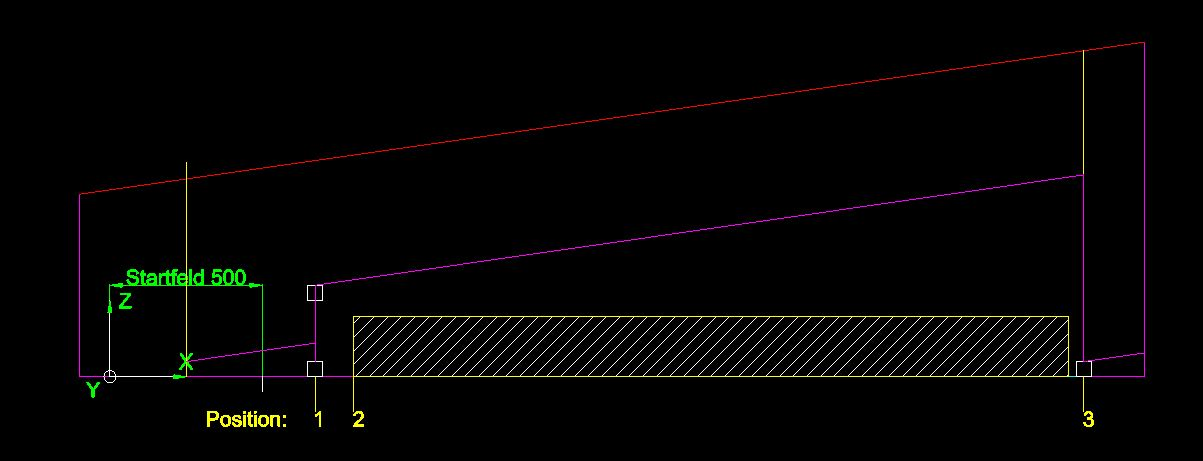
\includegraphics[keepaspectratio,height=4cm]{Teleskoparm1.JPG}
	\caption{Skizze Verfahrweg}
	\label{fig:Skizze Verfahrweg}
\end{figure}

Durch den Weg der die Last zurücklegen muss (violetter Pfad Abbildung \ref{fig:Skizze Verfahrweg}) ergeben sich zwei Extrempositionen.
(Seildurchhang wurde vernachlässigt)


\begin{itemize}[noitemsep]
	\item Position 2: Teleskoparm gestaucht
	\item Position 3: Teleskoparm maximal ausgefahren
\end{itemize}


\begin{figure}[h]
	\centering
	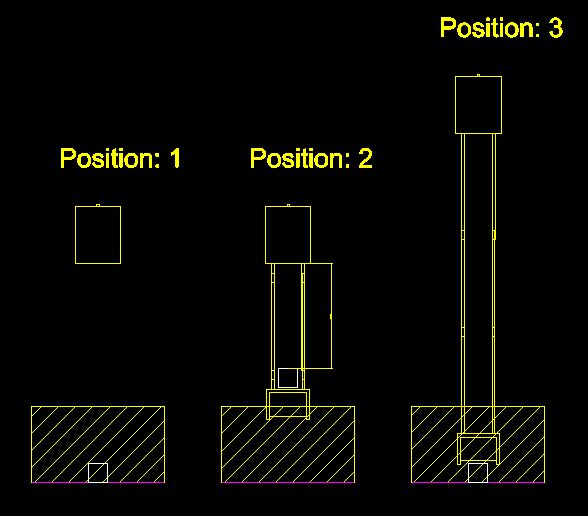
\includegraphics[keepaspectratio,height=4cm]{Teleskoparm2.JPG}
	\caption{Skizze Teleskop}
	\label{fig:Teleskoparm}
\end{figure}

Dabei wurde festgestellt, dass bei Position 2 wesentlich weniger Platz zwischen last und gerät vorhanden ist als bisher angenommen (Abbildung \ref{fig:Teleskoparm}). Bisher wurde mit einem Teleskop gerechnet, welcher aus 3-4 Segmenten besteht. Jedoch lässt sich dies nicht realisieren, da zu wenig Platz vorhanden ist. Für eine solche Lösung wäre ein Teleskop mit mehr als 8 Segmenten nötig. Dies wurde aufgrund des großen Aufwandes verworfen.

\subsection{Teleskop Variante 2}
\label{app:ssec:Teleskopje2}
Deshalb wurde eine Alternativlösung (Abbildung \ref{fig:Linearaufzug}) erarbeitet, bei der die Führungsstäbe nicht wie beim Teleskop eingefahren wird sondern seitwärts neben dem Antriebsmodul vorbei geschoben wird. Dies vereinfacht die bisherige Konstruktion zwar, jedoch muss der Abstand zwischen den Führungen genügend gross sein, dass die Antriebseinheit dazwischen platz hat.

\begin{figure}[h]
	\centering
	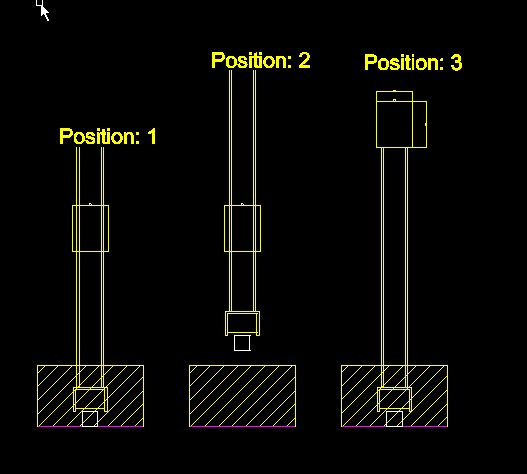
\includegraphics[keepaspectratio,height=4cm]{Teleskoparm3.JPG}
	\caption{Skizze Teleskoparm überarbeitet}
	\label{fig:Linearaufzug}
\end{figure}


\section{Durchhang}
\label{app:sec:Durchhang}
Der Durchhang des Seils ist abhängig vom Gewicht der Laufkatze. Dabei ist es wichtig den Durchhang für das sichere Überfahren der Hindernisse zu kennen. Zudem besteht die Möglichkeit, die Positionsanzeige in vertikaler Richtung als Funktion der zurückgelegten Strecke abzubilden, womit ein zusätzliches Messsystem weggelassen werden kann.

\subsection{Rechnung Durchhang}
\label{ssec:RechDurch}
Die Grundsteigung des Tragseils beträgt 8,2 Grad. Mithilfe von Trigonometrie und der Spannung des Seils konnte der Durchhang in der Mitte des Tragseils näherungsweise ausgerechnet werden.

\vspace{1em}
\noindent
\begin{table}[h!]
	\begin{tabular}{|p{0.15\textwidth}|p{0.2\textwidth}|p{0.55\textwidth}|}
		\hline
		\textbf{Gewicht [kg]} & \textbf{Steigungswinkel [\SI{}{\degree}](ohne Grundsteigung)} &\textbf{Durchhang [cm]}\\
		\hline
		0.5&0,95&2.29\\
		\hline
		1&1,91&5,84\\
		\hline
		1.5&2,87&8,76\\
		\hline
		2&3,82&11,69\\
		\hline
		2.5&4,78&14,63\\
		\hline
		3&5,74&17,59\\
		\hline
		3.5&6,70&20,56\\
		\hline
		4&7,66&23,54\\
		\hline
		4.5&8,63&26,55\\
		\hline
		5&9,59&29,58\\
		\hline
	\end{tabular}
	\caption{Rechnung Durchhang}
	\label{tbl:DurchhangRechnung}
\end{table}


\subsection{Grobversuch Durchhang}
\label{app:ssec:GrobeversDurch}
Es wurde ein einfacher Versuch über den Durchhang des Tragseiles gemacht. Die Dimensionen und Proportionen sind nicht massstäblich, nur Beispielhaft. Dabei wurde ein Seil zwischen zwei Stühlen durch ein Gewicht gespannt. Ein angebrachtes Gewicht wurde dannach an verschiedenen Positionen angehängt und der Durchhang wurde gemessen. Dabei kam raus, dass der maximale Durchhang in der Mitte des Tragseils ist. Der Durchhang im oberen fünftel des Tragseils betrug dabei ungefähr 2/3 des maximalen Durchhangs.
Für eine genaue Funktion des Durchhangs könnten am Musteraufbau Gewichte an verschiedenen Positionen angehängt und der Durchhang von Hand messen. Durch Eingabe in Excel kann somit die Funktion für verschiedene Gewichte ermittelt werden.

\chapter{Meilensteinberichte}
\label{app:ch:MeilensteinBerichte}

\includepdf[pages=1]{Meilensteinbericht_01.pdf}
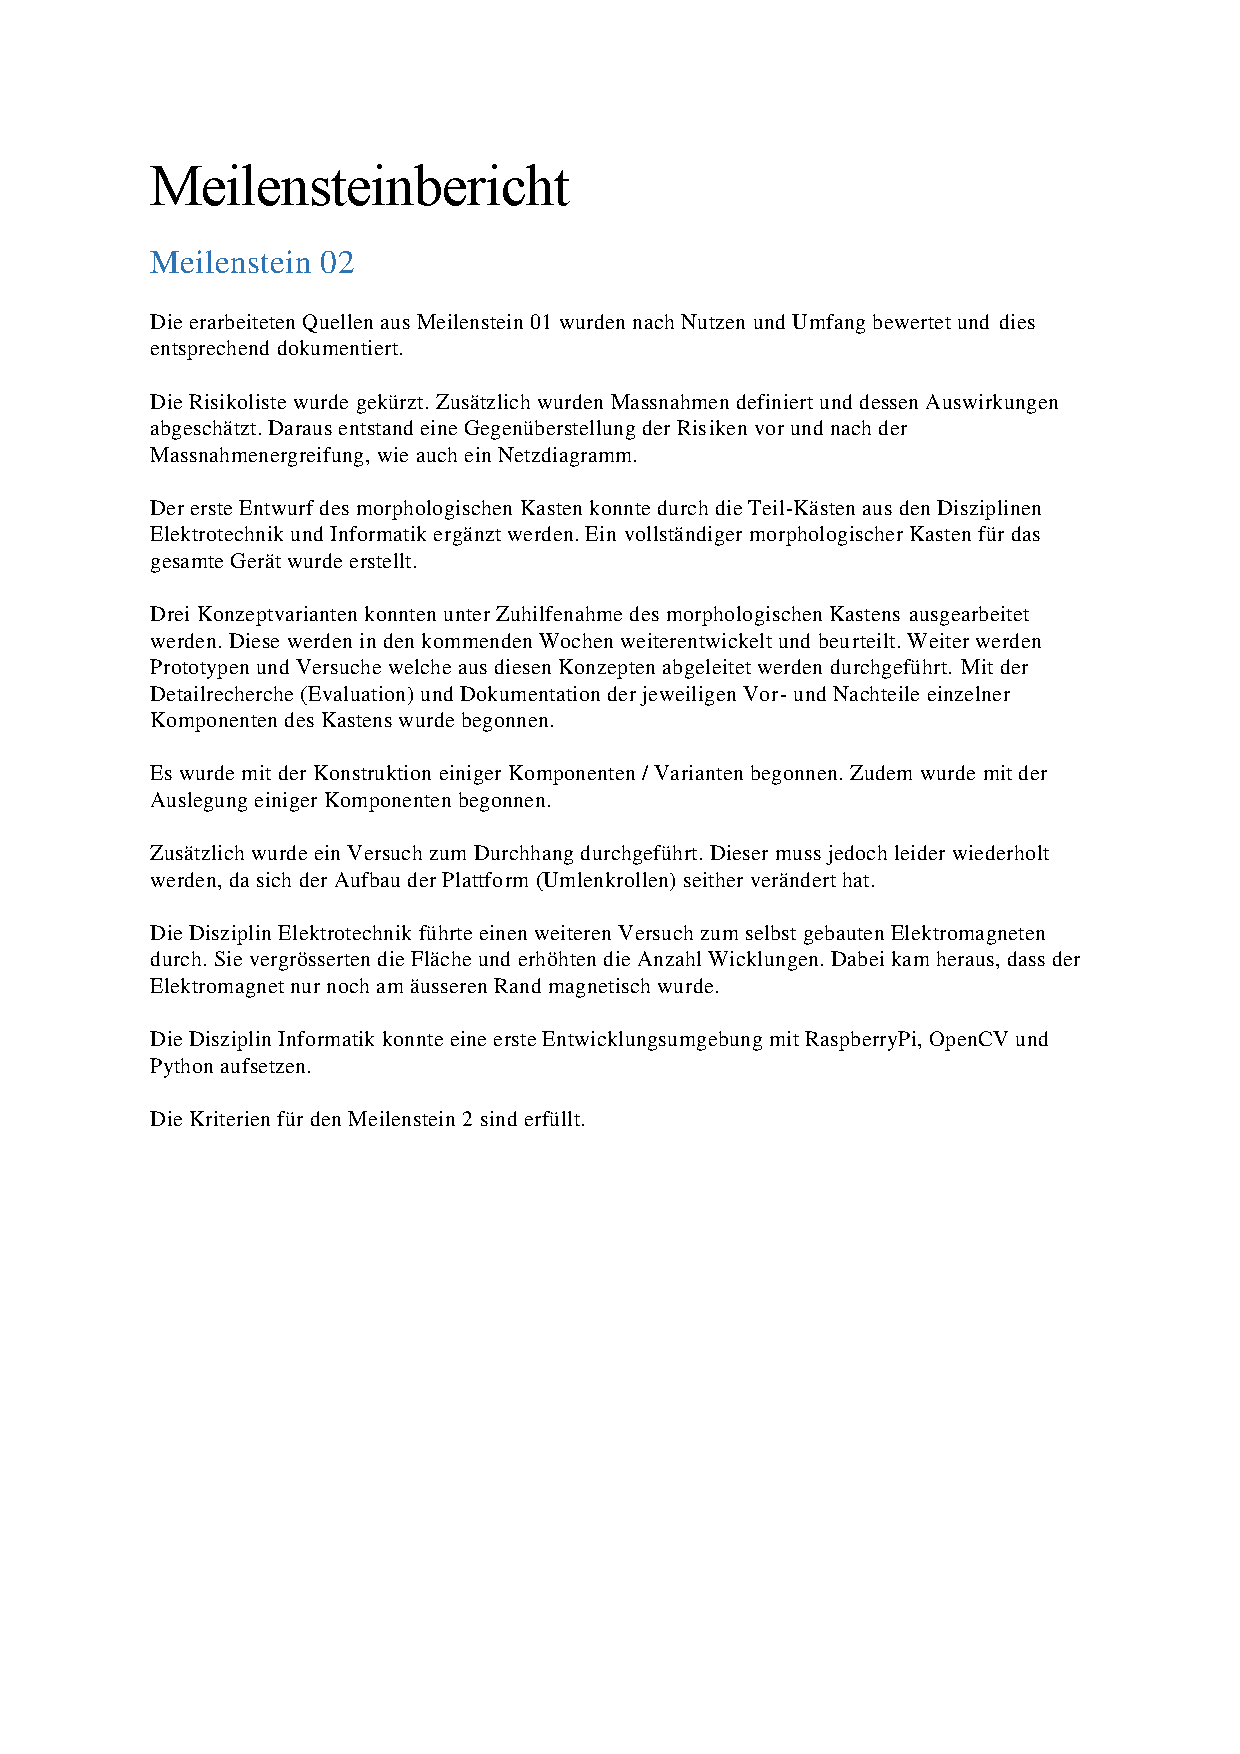
\includepdf[pages=1]{Meilensteinbericht_02.pdf}

\end{document}
